\chapter{Continuidad y límites de funciones}

\section{Definición de continuidad en un punto}\label{S:continuidad}

\subsection*{Intuición y precisión}

En esta sección hablaremos de manera intuitiva, y luego definiremos rigurosamente, el concepto de continuidad de una función $y=f(x)$.

Intuitivamente, la continuidad significa que un pequeño cambio en la variable independiente $x$ implica sólo un pequeño cambio en la variable dependiente $y=f(x)$, y excluye saltos en el valor de $y$; así, la gráfica consiste de un solo pedazo de curva. En contraste una gráfica $y=f(x)$ que consiste de pedazos de curvas separados por un vacío en una abscisa $x_0$ exhibe una \emph{discontinuidad de salto}. Por ejemplo, la función 
\begin{equation}\label{eq:signo}
f(x) = \sgn(x) = \begin{cases}
    -1, \quad &\text{si $x<0$},\\
    0, \quad &\text{si $x=0$},\\
    1, \quad &\text{si $x>0$},
\end{cases}
\end{equation}
Tiene una \emph{discontinuidad de salto} en $x_0 = 0$.

La idea de continuidad está implícita en el uso diario de las matemáticas. Muchas veces graficamos una función calculando el valor de la misma en algunos puntos y luego completamos el gráfico uniendo esos puntos.

La continuidad de la función $f(x)$ para un valor $x_0$ significa justamente que $f(x)$ difiere arbitrariamente poco del valor $f(x_0)$ cuando $x$ está suficientemente cerca de $x_0$. 
Las expresiones \emph{difiere arbitrariamente poco} y \emph{suficientemente cerca} son un tanto vagas y deben ser explicadas precisamente en términos cuantitativos.

Dado un \emph{margen de precisión} o \emph{tolerancia}, esto es, cualquier número real positivo $\epsilon$, para la continuidad de $f$ en $x_0$ se requiere que la diferencia entre $f(x)$ y $f(x_0)$ permanezca dentro de ese margen, esto es, que $|f(x)-f(x_0)|<\epsilon$, para todos los valores de $x$ que se encuentran suficientemente cercanos a $x_0$ (o bien, para todos los valores $x$ situados a una distancia menor que $\delta$ de $x_0$).

Es más fácil visualizar lo que la continuidad significa si se interpreta a $f$ como una transformación que asigna puntos $x$ en el eje $x$ en imágenes en el eje $y$.

\centerline{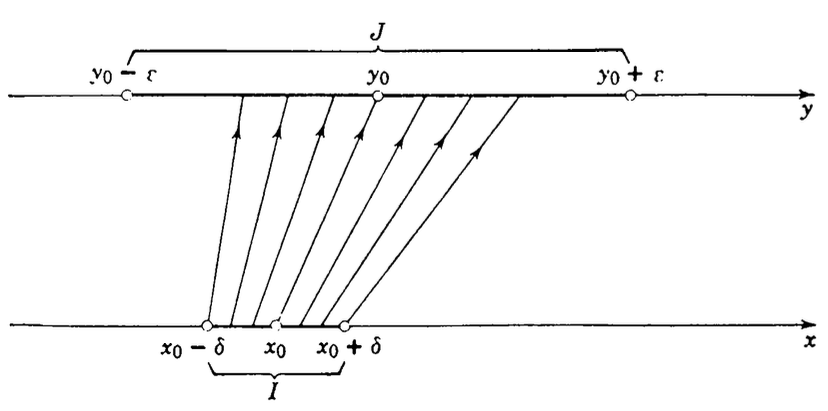
\includegraphics[width=.8\textwidth]{pics/continuidad-1.png}}

Tomemos cualquier punto $x_0$ en el eje $x$ y su imagen $y_0 = f(x_0)$. 
Marcamos un intervalo abierto, arbitrario $J$ en el eje $y$ que tiene al punto $y_0$ como centro; $J = (y_0-\epsilon,y_0+\epsilon) = \{ y \in \R : |y-y_0|<\epsilon\}$.
La condición para la continuidad de $f(x)$ en $x_0$ es: todos los puntos $x$ suficientemente cercanos a $x_0$ tienen imágenes que se encuentran en $J$. O bien: es posible marcar un intervalo $I$ en el eje $x$ con centro $x_0$, por ejemplo, el intervalo $x_0-\delta < x < x_0+\delta$, tal que todo punto $x$ de $I$ tiene una imagen $f(x)$ que se encuentra en $J$ y por lo tanto $|f(x)-f(x_0)|<\epsilon$.
La continuidad de $f(x)$ en el punto $x_0$ significa que para una $\epsilon$-\emph{vecindad} arbitraria $J$ del punto $y_0=f(x_0)$ en el eje $y$, puede encontrarse una $\delta$-vecindad $I$ del punto $x_0$ en el eje $x$, cuya totalidad de puntos son transformados por $f$ en puntos de $J$.
Por supuesto, esto solamente tiene sentido para puntos en el eje $x$ en los cuales la función está definida, esto es, los que pertenecen al dominio de $f$. Lo anterior nos conduce a la siguiente definición.

\begin{definition}\label{D:continuidad}
Sea $f$ definida en un intervalo abierto $(a,b)$ y sea $x_0\in(a,b)$.
    La función $f(x)$ es continua en $x_0$ si se cumple lo siguiente:
    \begin{quote}
        Para cada $\epsilon > 0$, existe $\delta > 0$ tal que
        \[ 
        |f(x) - f(x_0)| < \epsilon,
        \]
        para todos los valores $x$ que cumplen $|x-x_0|<\delta$.
    \end{quote}
\end{definition}

\begin{remark}
    Alternativamente, podemos decirlo de esta otra manera.
    La función $f(x)$ es continua en $x_0$ si se cumple lo siguiente:
    \begin{quote}
        Para cada $\epsilon > 0$, existe $\delta > 0$ tal que
        la imagen por $f$ del conjunto $(x_0-\delta,x_0+\delta)$ está contenida en $(f(x_0)-\epsilon,f(x_0)+\epsilon)$.
    \end{quote}

    O también suele escribirse así:
    La función $f(x)$ es continua en $x_0$ si se cumple lo siguiente:
    \begin{quote}
        Para cada $\epsilon > 0$, existe $\delta > 0$ tal que
        \[ 
        |x-x_0|<\delta \quad\implies\quad |f(x) - f(x_0)| < \epsilon.
        \]
    \end{quote}

\end{remark}

\begin{example}
    Veamos que la función $f(x)=5x+3$ es continua en $x_0 = 2$. Comenzamos, como cuando veíamos límite de sucesiones, analizando la expresión que queremos ver que sea menor a $\epsilon$:
    \[
    |f(x)-f(x_0)|      
    = |f(x)-f(2)|  
    = |(5x+3)-(5\cdot 2 + 3)|  
    = |5x-5\cdot 2 |
    = 5 \, |x-2|.
    \]
    Esta igualdad expresa que la transformación $y=5x+3$ \emph{magnifica} distancias por el factor $5$. Aquí vemos que $|f(x)-f(2)|<\epsilon$ si $5 |x-2| < \epsilon$, o lo que es lo mismo, si $|x-2|<\epsilon/5$.
    Por lo tanto, la condición para la continuidad en $x_0=2$ se verifica si se elige $\delta = \epsilon/5$.

    También podemos verificar que la misma función $f(x)=5x+3$ es continua en todo $x_0\in \R$. Con el mismo razonamiento,
    \[
    |f(x)-f(x_0)|  
    = |(5x+3)-(5 x_0 + 3)|  
    = |5x-5 x_0 |
    = 5 \, |x-x_0|.
    \]
    Luego, se cumplirá que $|f(x)-f(x_0)| <\epsilon$ si $5 \, |x-x_0|<\epsilon$, o lo que es lo mismo, si $|x-x_0|<\epsilon/5$.

    En ambos casos hemos demostrado que dado $\epsilon>0$ existe $\delta>0$ ($\delta=\epsilon/5$) tal que, 
    \[
    \text{si } |x-x_0|<\delta, \quad\text{entonces } |f(x)-f(x_0)|<\epsilon.
    \]
    Es decir, $f(x)=5x+3$ es continua en $x_0$, cualquiera sea $x_0\in\R$.
\end{example}

Veamos otro ejemplo, no tan sencillo.
\begin{example}
    Consideremos la función $f(x)=x^2$. Veamos que es continua en $x_0$ para cualquier $x_0\in\R$. Consideremos $x_0$ fijo, supongamos que $|x-x_0|<\delta$ y veamos qué tiene que cumplir $\delta$ para que se cumpla que $|f(x)-f(x_0)|<\epsilon$:
\begin{align*}
 |f(x)-f(x_0)|  
    &= |x^2 - x_0^2| = |x-x_0| \, |x+x_0|
    = |x-x_0| \, |(x-x_0)+2x_0|
    \\
    &\le |x-x_0| \big( |x-x_0|+2|x_0| \big)
    < \delta \big( \delta + 2 |x_0|\big).
\end{align*}
Ahora queremos elegir $\delta>0$ que asegure que $\delta \big( \delta + 2 |x_0|\big) < \epsilon$. No hace falta elegir el mejor $\delta$, uno que cumpla sería suficiente. Por ejemplo, si elegimos $\delta \le 1$, tenemos
que
\[
\delta \big( \delta + 2 |x_0|\big) \le \delta \big( 1 + 2 |x_0|\big)
< \epsilon, \quad\text{si } \delta \le \frac{\epsilon}{1 + 2 |x_0|}.
\]
Hechos estos \emph{cálculos auxiliares}, procedemos a demostrar que $f(x)=x^2$ es continua en todo punto $x_0$.

Sea $x_0\in\R$. Sea $\epsilon > 0$, arbitrario. Definimos $\delta = \min\{1,\frac{\epsilon}{1 + 2 |x_0|}\}$, de manera que $\delta\le 1$ y $\delta \le \frac{\epsilon}{1 + 2 |x_0|}$. Si $|x-x_0|<\delta$, entonces
\begin{align*}
 |f(x)-f(x_0)|  
    &= |x^2 - x_0^2| = |x-x_0| \, |x+x_0|
    = |x-x_0| \, |(x-x_0)+2x_0|
    \\
    &\le |x-x_0| \big( |x-x_0|+2|x_0| \big)
    < \delta \big( \delta + 2 |x_0|\big)
    \le \delta \big( 1 + 2 |x_0|\big)
< \epsilon.
\end{align*}
Resumiendo, hemos demostrado que dado $\epsilon > 0$, existe $\delta > 0$ tal que 
\[
|f(x)-f(x_0)|<\epsilon, \quad\text{para todo $x\in \R$ tal que $|x-x_0|<\delta$}.
\]
Es decir, $f(x)$ es continua en $x_0$.
\end{example}

\begin{remark}
    En el primer ejemplo, había que tomar $\delta = \frac\epsilon5$, y en el segundo $\delta = \min\{1,\frac{\epsilon}{1 + 2 |x_0|}\}$. Es interesante notar que, en el primer ejemplo, la misma elección de $\delta$ sirve para todo $x_0$, aunque depende de $\epsilon$. 
    En el segundo caso, $\delta$ depende de $\epsilon$ y también de $x_0$, ya que la transformación $y=x^2$ \emph{magnifica} distancias por un factor que no es el mismo para todo $x$.
\end{remark}

Intuitivamente, la idea de la continuidad parece obvia sin explicación, pero la formulación precisa puede ser en un principio algo difícil de entender debido a la variedad de palabras. 
Sin embargo, el lector, que puede estar al principio muy satisfecho con alguna noción intuitiva de la continuidad, aprenderá gradualmente a apreciar la lógica precisión y generalidad de la definición analítica, resultado de un largo y persistente esfuerzo para conciliar la necesidad de entendimiento intuitivo con el de la claridad lógica.
Es indispensable un significado preciso para la palabra continuidad. La definición dada aquí es la formulación requerida y precisa de una importante propiedad de las funciones.

\subsection*{Explicación de continuidad y discontinuidad mediante ejemplos}

Podemos aclarar la definición de continuidad, haciendo contraste con ejemplos de discontinuidad, ejemplos que no satisfacen la definición anterior. Recordemos el ejemplo sencillo de la función $f(x)=\sgn(x)$ en~\eqref{eq:signo}. Si hacemos un gráfico como el anterior, resulta así:

\centerline{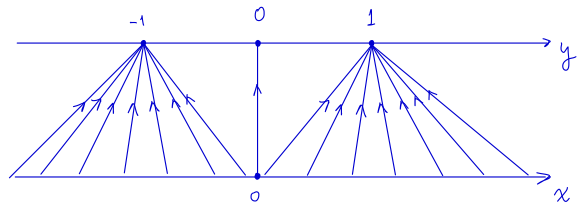
\includegraphics[width=.8\textwidth]{pics/signo.png}}

Esta función es continua en $x_0$, para todo $x_0\neq 0$. Para ver esto, analicemos por separado el caso $x_0>0$ y el caso $x_0<0$.

Sea $x_0 > 0$. Dado $\epsilon>0$, tomemos $\delta = x_0 = |x_0|$ (la distancia de $x_0$ al origen. Entonces, si $|x-x_0|<\delta=|x_0|$ resulta 
\[
0 = x_0-|x_0| < x < x_0+|x_0| = 2 \, |x_0|.
\]
Es decir, $x>0$, luego
\[
|\sgn(x)-\sgn(x_0)| = |1 - 1| = 0 < \epsilon.
\]
Sea ahora $x_0 <0$. Dado $\epsilon>0$, tomemos $\delta = -x_0 = |x_0|$ (la distancia de $x_0$ al origen). Entonces, si $|x-x_0|<\delta=|x_0|$ resulta 
\[
-2|x_0| = x_0-|x_0| < x < x_0+|x_0| = 0.
\]
Es decir, $x<0$, luego
\[
|\sgn(x)-\sgn(x_0)| = |(-1) - (-1)| = 0 < \epsilon.
\]
En síntesis, la función signo es continua en $x_0$, para $x_0>0$ y para $x_0<0$, dado que es constante en $(0,\infty)$ y en $(-\infty,0)$.

¿Qué ocurre en $x_0=0$?
En este caso $\sgn(x_0)=0$.
Para $\epsilon = 1/2$, cualquiera sea $\delta>0$, siempre existe un $x\in (x_0-\delta,x_0+\delta)=(-\delta,\delta)$ para el que $\sgn(x)=1$, por ejemplo, $x=\delta/2$, y para ese $x$ resulta
\[
|\sgn(x)-\sgn(x_0)| = |1 - 0| = 1 > \frac12=\epsilon.
\]

\centerline{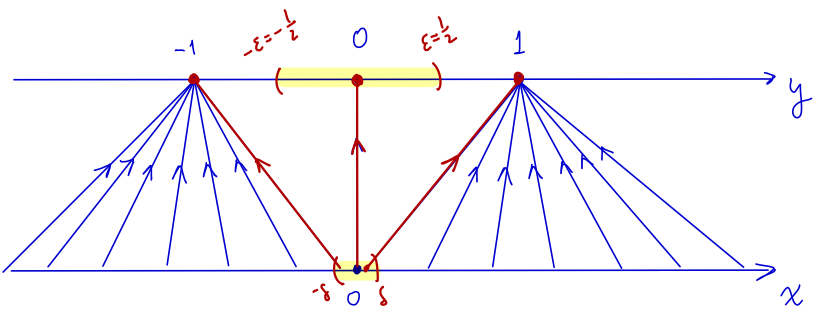
\includegraphics[width=.8\textwidth]{pics/signo-discontinuo.png}}

Es decir, no hay forma de elegir $\delta>0$ suficientemente pequeño para que la imagen por la función signo del intervalo $(-\delta,\delta)$ caiga dentro del intervalo $(-\epsilon,\epsilon)=(-1/2,1/2)$. De hecho, la imagen de $(-\delta,\delta)$ por la función $\sgn(x)$ es siempre el conjunto $\{-1,0,1\}$.

La discontinuidad de la función signo en $x_0=0$ es lo que se conoce como \emph{discontinuidad de salto}, ya que existen los \emph{límites laterales}.
Existe el límite de $f(x)$ cuando $x$ tiende a $0$ por derecha, y es igual a 1, y existe el límite de $f(x)$ cuando $x$ tiende a $0$ por izquierda, y es igual a $-1$. El \emph{salto} es la diferencia de estos límites.

Estamos hablando aquí del concepto de límite, pensando que se entiende intuitivamente lo que significa, pero ya haremos más rigurosa esta definición en la sección siguiente.

Hay otras discontinuidades que no son de salto, son las discontinuidades \emph{infinitas}, que son las que exhiben la función $f(x)=1/x^2$ y la $g(x)=1/x$.

\centerline{
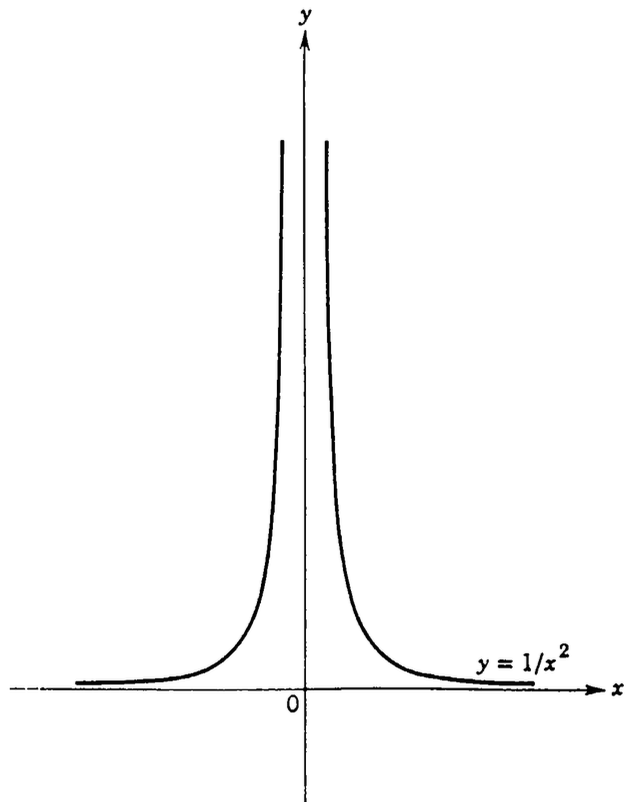
\includegraphics[width=.4\textwidth]{pics/discontinuidad-infinita.png}
\hfil
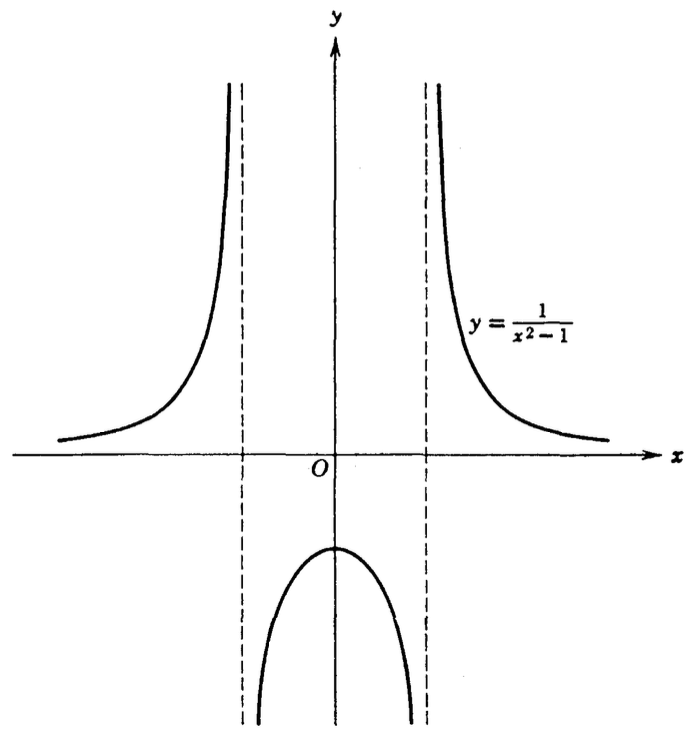
\includegraphics[width=.5\textwidth]{pics/dos-discontinuidades-infinitas.png}
}

A medida que $x$ se aproxima a cero, los valores de $f(x)=1/x^2$ crecen más allá de toda cota. En este caso, diremos que $\D\lim_{x\to0} \frac1{x^2}=\infty.$

\subsubsection*{Ejercicios de la sección~\getcurrentref{chapter}.\getcurrentref{section}}


\begin{enumerate}
\item Demostrar que la función $f(x)=-3x+10$ es continua en $x_0$, para todo $x_0\in\R$.

\item 
Consideremos la función $f:(0,\infty)\to(0,\infty)$ dada por
$f(x)=\frac1x$.
\begin{enumerate}
    \item Demostrar que es continua en $x_0=2$;
    \item Demostrar que es continua en $x_0=1$;
    \item Demostrar que es continua en $x_0=1/2$;
    \item ¿Se anima a demostrar que es continua en $x_0$, cualquiera sea  $x_0>0$?
\end{enumerate}

\item 
Consideremos la función $f:(0,\infty)\to(0,\infty)$ dada por
$f(x)=\sqrt x$.
\begin{enumerate}
    \item Demostrar que es continua en $x_0=2$;
    \item Demostrar que es continua en $x_0=1$;
    \item Demostrar que es continua en $x_0=1/2$;
    % \item Demostrar que es continua en $x_0=0$;
    \item ¿Se anima a demostrar que es continua en $x_0$, cualquiera sea $x_0\in(0,\infty)$?
\end{enumerate}

\item 
Consideremos la función 
\[
f(x) = \begin{cases}
    x\sen \frac1x,\quad &\text{si $x\neq 0$},
    \\
    0,\quad &\text{si $x = 0$},
    \end{cases}
\]
\begin{enumerate}
    \item Graficarla con GeoGebra
    \item Verificar con geogebra que 
    \[
    -|x| \le f(x) \le |x|,\quad \forall\xiR.
    \]
    \item Demostrar analíticamente que 
    \[
    -|x| \le f(x) \le |x|,\quad \forall\xiR.
    \]
    \item Verificar que $|f(x)-f(0)|\le |x-0|$, para todo \xiR.
    \item Demostrar que $f(x)$ es continua en $x_0=0$.
\end{enumerate}

\item 
Consideremos la función
\[
H(x) = \begin{cases}
    0, \quad &\text{si $x<0$},\\
    1, \quad &\text{si $x\ge0$},
\end{cases}
\]
\begin{enumerate}
    \item Demostrar que $H(x)$ es continua en $x_0$ para todo $x_0\neq 0$.
    \item Demostrar que $H(x)$ no es continua en $x_0=0$.
\end{enumerate}

\item \label{ej:sen1_x}
Consideremos la función 
\[
f(x) = \begin{cases}
    \sen \frac1x,\quad &\text{si $x\neq 0$},
    \\
    0,\quad &\text{si $x = 0$},
    \end{cases}
\]
\begin{enumerate}
    \item Graficarla con GeoGebra
    \item Demostrar que para cada $\delta>0$ existe $x_1\in(0,\delta)$ tal que $f(x_1)=1$.
    \item Demostrar que para cada $\delta>0$ existe $x_2\in(0,\delta)$ tal que $f(x_2)=-1$.
    \item Demostrar que $f(x)$ no es continua en $x_0=0$.
\end{enumerate}


\end{enumerate}

\section{Propiedades de funciones continuas en un punto}\label{S:continuidad-propiedades}

A continuación veremos algunas propiedades que cumplen las funciones alrededor de un punto de continuidad.

\begin{proposition}\label{P:continua:cota en intervalo}
    Sea $f$ continua en $x_0$. Si $a<f(x_0)<b$, entonces existe $\delta>0$ tal que 
    \[
    a<f(x)<b, \quad\text{para todo $x\in (x_0-\delta,x_0+\delta)$}.
    \]
\end{proposition}

\begin{proof}
    Basta con tomar $\epsilon=\min\{b-f(x_0),f(x_0)-a\}$ en la definición de continuidad, y elegir el $\delta$ que le corresponde.
\end{proof}

Como consecuencia de esta proposición tenemos que si $f$ es continua en $x_0$ y $f(x_0)>0$, entonces $f$ es positiva en todo un entorno que contiene a $x_0$. Más precisamente, existe $\delta>0$ tal que $f(x)>0$ para todo $x\in (x_0-\delta,x_0+\delta)$.

\begin{proposition}
    Si $f$ y $g$ son continuas en $x_0$, entonces $f+g$ es continua en $x_0$.
\end{proposition}

\begin{proof}
Sea $\epsilon >0$.
Como $f$ es continua en $x_0$ existe $\delta_f>0$ tal que 
\[
|f(x)-f(x_0)|<\frac\epsilon2, \quad\text{para todo $x\in(x_0-\delta_f,x_0+\delta_f)$}.
\]
Como $g$ es continua en $x_0$ existe $\delta_g>0$ tal que 
\[
|g(x)-g(x_0)|<\frac\epsilon2, \quad\text{para todo $x\in(x_0-\delta_g,x_0+\delta_g)$}.
\]
Tomemos ahora $\delta=\min\{\delta_f,\delta_g\}$. Si $x\in(x_0-\delta,x_0+\delta)$, entonces $x\in(x_0-\delta_f,x_0+\delta_f)\cap(x_0-\delta_g,x_0+\delta_g)$.
Por lo tanto, 
\begin{align*}
\Big|\big(f(x)+g(x)\big)-\big(f(x_0)+g(x_0)\big)\Big|
&=\Big|\big(f(x)-f(x_0)\big)+\big(g(x)-g(x_0)\big)\Big|
\\
&\le \big|f(x)-f(x_0)\big|+\big|g(x)-g(x_0)\big|
<\frac\epsilon2+\frac\epsilon2=\epsilon,
\end{align*}
para todo $x\in(x_0-\delta,x_0+\delta)$.

Hemos demostrado que dado $\epsilon>0$, existe $\delta>0$ tal que 
\[
\Big|\big(f(x)+g(x)\big)-\big(f(x_0)+g(x_0)\big)\Big|
<\epsilon , \quad\text{para todo $x\in(x_0-\delta,x_0+\delta)$}.
\]
Es decir, $f+g$ es continua en $x_0$.
\end{proof}


\begin{proposition}
    Si $f$ y $g$ son continuas en $x_0$, entonces $f\cdot g$ es continua en $x_0$.
\end{proposition}

\begin{proof}
    Comencemos observando la diferencia que queremos hacer menor a $\epsilon$:
\begin{align*}
\big|f(x) g(x)-f(x_0) g(x_0)\big|
&=
\big|f(x) g(x)-f(x_0) g(x)+f(x_0) g(x)-f(x_0) g(x_0)\big|
\\
&\le 
\big|f(x) g(x)-f(x_0) g(x)\big|+\big|f(x_0) g(x)-f(x_0) g(x_0)\big|
\\
&\le 
\big|f(x)-f(x_0)\big|\,\big|g(x)\big|+\big|f(x_0)\big| \, \big| g(x)- g(x_0)\big|.
\end{align*}
Vemos que aparecen $|f(x)-f(x_0)|$ y $|g(x)- g(x_0)|$ que podremos acotar por $\epsilon$, pero multiplicados por $|g(x)|$ y por $|f(x_0)|$.
Como $|g(x)|$ todavía depende de $x$ y \emph{no está fijo} debemos acotarlo primero.

Observemos que como $g$ es continua en $x_0$, tomando $\epsilon=1$ en la definición, resulta que existe $\delta_1>0$ tal que
\[
|g(x)-g(x_0)|<1, \quad\text{para todo $x\in(x_0-\delta_1,x_0+\delta_1)$}.
\]
Esto implica que 
\[
|g(x)| < |g(x_0)|+1,  \quad\text{para todo $x\in(x_0-\delta_1,x_0+\delta_1)$}.
\]

Sea ahora $\epsilon>0$ arbitrario.
Llamamos $M=|g(x_0)|+1$ y $N=|f(x_0)|+1$. 
Como $f$ es continua en $x_0$ existe $\delta_f>0$ tal que 
\[
|f(x)-f(x_0)|<\frac{\epsilon}{2M}, \quad\text{para todo $x\in(x_0-\delta_f,x_0+\delta_f)$}.
\]
Como $g$ es continua en $x_0$ existe $\delta_g>0$ tal que 
\[
|g(x)-g(x_0)|<\frac\epsilon{2N}, \quad\text{para todo $x\in(x_0-\delta_g,x_0+\delta_g)$}.
\]

Tomemos ahora $\delta=\min\{\delta_1,\delta_f,\delta_g\}$. Luego,
\[
\text{si $x\in (x_0-\delta,x_0+\delta)$}
\quad\implies\quad
x\in(x_0-\delta_1,x_0+\delta_1)\cap(x_0-\delta_f,x_0+\delta_f)\cap(x_0-\delta_g,x_0+\delta_g).
\]
Por lo tanto, para $x\in (x_0-\delta,x_0+\delta)$ se tiene que
\begin{align*}
\big|f(x) g(x)-f(x_0) g(x_0)\big|
&\le 
\big|f(x)-f(x_0)\big|\,\big|g(x)\big|+\big|f(x_0)\big| \, \big| g(x)- g(x_0)\big|
\\
&< \frac{\epsilon}{2M} M + N \frac\epsilon{2N} = \frac\epsilon2+\frac\epsilon2=\epsilon.
\end{align*}

Hemos demostrado que dado $\epsilon>0$ existe $\delta>0$ tal que
\[
\big|f(x) g(x)-f(x_0) g(x_0)\big|<\epsilon, \quad\text{para todo $x\in(x_0-\delta,x_0+\delta)$}.
\]
Es decir, $fg$ es continua en $x_0$.
\end{proof}

\begin{proposition}
    Si $f$ y $g$ son continuas en $x_0$, 
    y si además $g(x_0)\neq 0$, entonces $f/g$ es continua en $x_0$.
\end{proposition}

\begin{proof}
    Veamos primero que si $g$ es continua en $x_0$ y $g(x_0)\neq 0$, entonces $\D\frac1g$ es continua en $x_0$.
    Para esto, observemos que
    \begin{align*}
        \Big| \frac1{g(x)}-\frac1{g(x_0)} \Big| 
        &= 
        \Big| \frac{g(x_0)-g(x)}{g(x)\,g(x_0)} \Big| 
        = 
         \frac{1}{|g(x)\,g(x_0)|}
        \big| g(x_0)-g(x) | .
    \end{align*}
    Sin pérdida de generalidad, supongamos que $g(x_0)>0$ (el caso $g(x_0)<0$ es análogo).
    Como $g(x_0)>0$, resulta que $0<\frac{g(x_0)}{2}<g(x_0)$. 
    Por la Proposición~\ref{P:continua:cota en intervalo}, existe $\delta_1>0$ tal que 
\[
g(x)>\frac{g(x_0)}2,  \quad\text{para todo $x\in(x_0-\delta_1,x_0+\delta_1)$}.
\] 
Luego, 
\[
\frac{1}{|g(x)\,g(x_0)|} = \frac{1}{g(x)\,g(x_0)}
< \frac{2}{g(x_0)\,g(x_0)}
= \frac{2}{g(x_0)^2},  \quad\text{para todo $x\in(x_0-\delta_1,x_0+\delta_1)$}.
\] 

Sea ahora $\epsilon>0$ arbitrario.
Llamamos $M=\frac{2}{g(x_0)^2}$.
Como $g$ es continua en $x_0$ existe $\delta_g>0$ tal que 
\[
|g(x)-g(x_0)|<\frac\epsilon{M}, \quad\text{para todo $x\in(x_0-\delta_g,x_0+\delta_g)$}.
\]
Tomemos ahora $\delta=\min\{\delta_1,\delta_g\}$. Luego,
\[
\text{si $x\in (x_0-\delta,x_0+\delta)$}
\quad\implies\quad
x\in(x_0-\delta_1,x_0+\delta_1)\cap(x_0-\delta_g,x_0+\delta_g).
\]
Por lo tanto, para $x\in (x_0-\delta,x_0+\delta)$ se tiene que
    \begin{align*}
        \Big| \frac1{g(x)}-\frac1{g(x_0)} \Big| 
        &= 
         \frac{1}{|g(x)\,g(x_0)|}
        \big| g(x_0)-g(x) | 
        < M \frac{\epsilon}M = \epsilon
    \end{align*}

Hemos demostrado que dado $\epsilon>0$ existe $\delta>0$ tal que
\[
        \Big| \frac1{g(x)}-\frac1{g(x_0)} \Big| <\epsilon,
        \quad\text{para todo $x\in(x_0-\delta,x_0+\delta)$}.
\]
Es decir, $\D\frac1g$ es continua en $x_0$.

Finalmente, $\D\frac fg = f \frac1g$. Como $f$ y $\D\frac1g$ son continuas en $x_0$, también lo es su producto por la proposición anterior.
\end{proof}

La siguiente proposición dice que si dos funciones son continuas, entonces también es continua su composición.

\begin{proposition}
    Si $g$ es continua en $x_0$ y $f$ es continua en $g(x_0)$, entonces $f\circ g$ es continua en $x_0$.
\end{proposition}

\begin{proof}
Esta demostración es un poquito más difícil, pero no tanto.
Para hacerla, llamaremos $y$ a la variable independiente de la función $f$.

Sea $\epsilon>0$, como $f$ es continua en $y_0=g(x_0)$, existe $\eta>0$ tal que
\[
|f(y)-f(y_0)|<\epsilon, \quad\text{para todo $y\in(y_0-\eta,y_0+\eta)$},
\]
es decir
\begin{equation}\label{P:composicion-intermedio}
|f(y)-f(y_0)|<\epsilon, \quad\text{si $|y-y_0|<\eta$},
\end{equation}
También hemos utilizado la letra griega $\eta$ (``eta'') en lugar de $\delta$, pero esto no es un problema.

\comentario{Como $\eta>0$, podemos utilizarla en lugar de $\epsilon$ en la definición de continuidad de $g$ en $x_0$.}

Como $g$ es continua en $x_0$ y $\eta>0$, existe $\delta>0$ tal que 
\[
|\underbrace{g(x)}_y-\underbrace{g(x_0)}_{y_0}|<\eta, \quad\text{para todo $x\in(x_0-\delta,x_0+\delta)$}.
\]
Si ahora $x\in(x_0-\delta,x_0+\delta)$, resulta que $y=g(x)$ cumple $|y-y_0|<\eta$ y por lo tanto, de~\eqref{P:composicion-intermedio} tenemos que
\[
|f\circ g(x)-f\circ g(x_0) | 
=\big|f\big(g(x)\big)-f\big(g(x_0)\big) \big| 
=\big|f\big(y\big)-f\big(y_0\big) \big| <\epsilon.
\]

Hemos demostrado que dado $\epsilon>0$ existe $\delta>0$ tal que
\[
        |f\circ g(x)-f\circ g(x_0) |  <\epsilon,
        \quad\text{para todo $x\in(x_0-\delta,x_0+\delta)$}.
\]
Es decir, $f\circ g$ es continua en $x_0$.
\end{proof}

Para continuar hablando de continuidad, conviene introducir el concepto de límite de funciones, lo que haremos en la siguiente sección.

\subsubsection*{Ejercicios de la sección~\getcurrentref{chapter}.\getcurrentref{section}}

\begin{enumerate}
\item Consideremos la función constante $f(x)=a$, para algún $a\in\R$. Demostrar usando la definición que $f$ es continua en $x_0$ para todo $x_0\in\R$.
\item Consideremos la función \emph{identidad} $f(x)=x$. Demostrar usando la definición que $f$ es continua en $x_0$ para todo $x_0\in\R$.
\item Demostrar que si $a$ y $b$ son números reales, entonces la función lineal $f(x)=ax+b$ es continua en $x_0$ para todo $x_0\in\R$.
Usar lo demostrado en los ejercicios anteriores y las propiedades vistas en esta sección.
\item Demostrar que si $a$, $b$ y $c$ son números reales, entonces la función cuadrática $f(x)=ax^2+bx+c$ es continua en $x_0$ para todo $x_0\in\R$.
Usar lo demostrado en los ejercicios anteriores y las propiedades vistas en esta sección.
\item\label{ej:polinomios-continuos} Demostrar que si $p(x)$ es una función polinomial, entonces $p$ es continua en $x_0$ para todo $x_0\in\R$ (Ayuda: usar inducción sobre el grado polinomial).
\item Demostrar que si $p(x)$ y $q(x)$ son funciones polinomiales, entonces la función racional $\frac pq$ es continua en $x_0$ para todo $x_0\in\R$, excepto para aquellos puntos donde $q(x)$ se anula. 


\end{enumerate}


\section{Límites por la derecha}

\subsection{Definición y ejemplos}

Hemos hablado en la sección anterior muy brevemente sobre el concepto de límite. En esta sección presentaremos la definición rigurosa de este concepto y veremos algunos ejemplos.

La idea intuitiva de \emph{límite} de una función $f(x)$ cuando $x$ se acerca a $x_0$ \emph{por derecha}, es el número al que se acercan los valores de $f(x)$ cuando $x$ está arbitrariamente cerca de $x_0$, pero a la derecha de $x_0$, es decir, $x>x_0$. Es importante notar que aquí hemos escrito $x>x_0$ y no $x\ge x_0$. Esto es así, porque no queremos saber el valor de $f(x_0)$, sino el valor al que se acerca $f(x)$ cuando $x$ está cerca de $x_0$, pero $x\neq x_0$.

Por ejemplo, en la función $f(x)=\sgn(x)$ dada en~\eqref{eq:signo}, diremos que límite de $\sgn(x)$ cuando $x$ tiende a cero por derecha es 1, que difiere de $\sgn(0)=0$. En símbolos, escribiremos $\D\lim_{x\to0^+} \sgn(x)=1$.

\begin{definition}[Límite por la derecha]
    Sea $x_0\in\R$ y sea $f$ una función definida en un intervalo $(x_0,x_0+c)$, con $c>0$. Se dice que límite de $f(x)$ cuando $x$ tiende a $x_0$ por derecha es $\ell$ y se escribe
    \[
    \lim_{x\to x_0^+}f(x)=\ell,
    \]
    cuando se cumple lo siguiente:
    \begin{quote}
        Dado $\epsilon > 0$, existe $\delta > 0$ tal que 
        \[
        |f(x)-\ell| < \epsilon, \quad\text{para todo $x\in (x_0,x_0+\delta)$}
        .
        \]
    \end{quote}
\end{definition}
    
\begin{remark}
    En otras palabras
    \[
    \lim_{x\to x_0^+}f(x)=\ell,
    \]
    cuando se cumple lo siguiente:
    \begin{quote}
        Dado $\epsilon > 0$, existe $\delta > 0$ tal que 
        \[
        x_0<x<x_0+\delta
        \quad\implies\quad |f(x)-\ell| < \epsilon.
        \]
    \end{quote}
\end{remark}

\begin{example}
Veamos que con esta definición es cierto que $\D\lim_{x\to0^+} \sgn(x)=1$.
Como la función es constantemente igual a 1 para $x>0$, la elección de $\delta$ será muy sencilla; en realidad cualquier $\delta>0$ sirve, pero para ser explícitos, tomaremos $\delta=1$.\footnote{Queremos evitar aquí el problema que le surgió a Homero Simpson, cuando la computadora le pedía que ``TO START PRESS ANY KEY", y no encontraba la tecla ``ANY"  (\url{https://www.youtube.com/watch?v=st6-DgWeuos}\quad:-)}

Sea $\epsilon > 0$, tomemos $\delta=1$, luego, si $0<x<\delta=1$, resulta que
\[
|\sgn(x)-1| = |1-1|=0<\epsilon,
\]
donde hemos utilizado solamente que $x>0$, ignorando que $x<1$.
Hemos demostrado entonces que dado $\epsilon>0$ existe $\delta>0$ con la propiedad de que
\[
0<x<0+\delta \quad\implies\quad |\sgn(x)-1|<\epsilon,
\]
es decir, $\D\lim_{x\to0^+} \sgn(x)=1$.
\end{example}

\begin{example}
Consideremos la función $f:\R\to\R$ definida por $f(x)=\lfloor x\rfloor$, la función \emph{parte entera de $x$}, o también llamada \emph{piso de $x$}.
Es decir, $f(x)$ es el único entero que cumple $f(x)\le x< f(x)+1$. Así, $f(x)=0$, para todo $x\in[0,1)$, $f(x)=1$, para todo $x\in[1,2)$, etc. En general
\[
f(x)=n, \qquad \text{si }n\in\Z \quad\text{y}\quad n\le x < n+1.
\]
Veamos que el límite de $f(x)$ cuando $x$ tiende a $3$ por derecha es $3$, es decir, $\lim_{x\to 3^+}f(x)=3$.
Observamos que $f$ es constante en el intervalo $[3,4)$, por lo tanto, lo que ocurre es similar a lo que ocurre con la función signo.
Sea $\epsilon>0$, elegimos $\delta=1$ y observamos que si $3<x<3+\delta=4$ entonces $f(x)=3$,
por lo tanto
\[
|f(x)-3| = |3-3|=0<\epsilon,\quad\text{para todo $x\in (3,3+\delta)$}.
\]
De la misma manera, cambiando $3$ por $n$ y $4$ por $n+1$ podemos probar que si $n\in\Z$, entonces $\lim_{x\to n^+}f(x)=n$.

Consideremos ahora un número $x_0\in \R\setminus\Z$, es decir, $x_0$ es real, pero no entero. Entonces, si tomamos $n=\lfloor x_0 \rfloor$, resulta que
$n\in\Z$ y $n<x_0<n+1$, donde ambas desigualdades son \emph{estrictas}, porque $x_0$ no es entero.
Además, $f(x_0)=n$, y si ampliamos el gráfico alrededor del punto $(x_0,n)=(x_0,f(x_0))$, vemos que la función $f$ es constante alrededor de $x_0$.
Dado $\epsilon>0$, ?`cómo tenemos que elegir $\delta>0$ de manera de asegurarnos que $|f(x)-f(x_0)|<\epsilon$ para todo $x\in(x_0,x_0+\delta)$?
Bien, tenemos que asegurarnos que si $x\in(x_0,x_0+\delta)$ entonces $x$ \emph{no se pase a la derecha de $n+1$}.
Para eso, podemos definir $\delta=n+1-x_0$ que es positivo porque ya dijimos que $x_0<n+1$. Luego, si
$x\in(x_0,x_0+\delta)$, resulta $x_0<x<x_0+\delta = x_0+(n+1-x_0)=n+1$, es decir $x_0<x<n+1$ y por lo tanto $f(x)=\lfloor x \rfloor = n = f(x_0)$, que a su vez implica
\[
|f(x)-f(x_0)|=|n-n|=0<\epsilon.
\]
Por lo tanto, dado $\epsilon>0$ existe $\delta=n+1-x_0>0$ tal que $|f(x)-f(x_0)|<\epsilon$ para todo $x\in(x_0,x_0+\delta)$. Es decir, $\lim_{x\to x_0^+}f(x)=f(x_0)$.
\end{example}

\begin{example}
    Consideremos ahora la función definida por $f(x)=\frac{4x^2-100}{x-5}$ cuyo dominio es $\R\setminus\{5\}$.
    Igualmente podemos calcular el límite de $f(x)$ cuando $x$ tiende a $5$ por derecha.
    Afirmamos que $\lim_{x\to 5^+} f(x) = 40$. Esto surge de observar que si $x\neq 5$, entonces
    \[
    f(x) = \frac{4x^2-100}{x-5} = 4\frac{x^2-5^2}{x-5} = 4\frac{(x-5)(x+5)}{x-5} = 4(x+5)\qquad\text{(para $x\neq 5$).}
    \]
    
    Es decir, $f(x)=4(x+5)$, para $x\neq 5$. Si miramos esta fórmula para $x$ cercano a 5, vemos que los valores $4(x+5)$ están cercanos a $4(5+5)=40$.
    Veamos que se cumple la definición formal.
    Sea $\epsilon > 0$, supongamos que $5<x<5+\delta$, es decir $0<x-5<\delta$ y veamos qué ocurre con $|f(x)-40|$. Queremos descubrir qué tiene que cumplir $\delta$ para que $|f(x)-40|<\epsilon$:
    \[
    |f(x)-40|=\left|\frac{4x^2-100}{x-5}-10\right|=|4(x+5)-40|=|4x-20|=4(x-5)<4\delta.
    \]
    Si tomamos $\delta=\epsilon/4$ (para que $4\delta=\epsilon$) resultará que
    \[
    |f(x)-40| < \epsilon, \qquad\text{para todo $x \in (5,5+\delta)$}.
    \]
    Hemos demostrado que dado $\epsilon > 0$ existe $\delta=\epsilon/4$ tal que $|f(x)-40| < \epsilon$, para todo $x \in (5,5+\delta)$.
    Es decir, $\lim_{x\to 5^+} f(x) = 40$.
\end{example}

Terminamos esta sección probando dos propiedades que parecen obvias, pero nos permiten practicar y asimilar la definición de límite.

\begin{lemma}
    Si $f$ es la función \emph{constante}, $f(x)=c$, para todo $x\in\R$, entonces 
    \[ 
    \lim_{x\to x_0^+} f(x) = c, \qquad\text{cualquiera sea $x_0\in\R$}.
    \]
\end{lemma}

\begin{proof}
    Dado $\epsilon>0$, elegimos $\delta=1$ y se cumple que
    \[
    |f(x)-c|=|c-c|=0<\epsilon, \quad\text{para todo $x\in(x_0,x_0+\delta)$}.
    \qedhere \]
\end{proof}

\begin{proposition}
    Si $\lim_{x\to x_0^+} f(x) = \ell$, entonces $\lim_{x\to x_0^+} |f(x)|=|\ell|$.
\end{proposition}

\begin{proof}
    Como $\limxo f(x)=\ell$, dado $\epsilon>0$ existe $\delta>0$ tal que $| f(x)-\ell |<\epsilon$ para todo $x\in(x_0,x_0+\delta)$.
    Pero entonces, si $x\in(x_0,x_0+\delta)$, por la desigualdad triangular, resulta que
    \[
    \big| |f(x)|-|\ell| \big| \le \big| f(x)-\ell \big|<\epsilon.
    \qedhere
    \]
\end{proof}


\subsection{Propiedades del límite por la derecha}


A continuación veremos algunas propiedades del límite que nos permitirán calcularlos sin necesidad de recurrir siempre a la definición.

\begin{proposition}[Unicidad del límite]
    Sea $f$ definida en $(x_0,x_0+c)$ para algún $c>0$. Si $\ell_1$ y $\ell_2$ cumplen que
    \[
    \lim_{x\to x_0^+} f(x)=\ell_1, 
    \qquad \text{y}\qquad 
    \lim_{x\to x_0^+} f(x)=\ell_2,
    \]
    entonces $\ell_1=\ell_2$.
\end{proposition}

\begin{proof}
Sea $\epsilon>0$. 
Como $\lim_{x\to x_0^+} f(x)=\ell_1$, existe $\delta_1$ tal que
\[
|f(x)-\ell_1| < \frac{\epsilon}2, \qquad\text{ para todo $x\in(x_0,x_0+\delta_1)$}.
\]
Como $\lim_{x\to x_0^+} f(x)=\ell_2$, existe $\delta_1$ tal que
\[
|f(x)-\ell_2| < \frac{\epsilon}2, \qquad\text{ para todo $x\in(x_0,x_0+\delta_2)$}.
\]
Si ahora $x\in(x_0,x_0+\min\{\delta_1,\delta_2\}$ tenemos que 
\[
|f(x)-\ell_1| < \frac{\epsilon}2
\quad\text{y}\quad
|f(x)-\ell_2| < \frac{\epsilon}2.
\]
Entonces
\begin{align*}
|\ell_1-\ell_2|&=|\ell_1-f(x)+f(x)-\ell_2|
\le |\ell_1-f(x)|+|f(x)-\ell_2|
\\
&= |f(x)-\ell_1|+|f(x)-\ell_2|
< \frac\epsilon2+\frac\epsilon2=\epsilon.
\end{align*}

Hemos demostrado que $|\ell_1-\ell_2|<\epsilon$, para todo $\epsilon>0$.
Luego $|\ell_1-\ell_2|=0$, o lo que es lo mismo $\ell_1=\ell_2$.
\end{proof}

\begin{proposition}\label{P:limite implica valores acotados}
    Supongamos que $\lim_{x\to x_0^+} f(x)=\ell$.
    \begin{enumerate}
        \item Si $\ell<b$, existe $\delta>0$ tal que $f(x)<b$, para todo $x\in(x_0,x_0+\delta)$.
        \item Si $\ell>b$, existe $\delta>0$ tal que $f(x)>b$, para todo $x\in(x_0,x_0+\delta)$.
    \end{enumerate}
\end{proposition}

\begin{proof}
Basta con tomar $\epsilon = |b-\ell|$ en la definición de límite.
\end{proof}

\begin{theorem}[Teorema del Emparedado]
    Sean $f$, $g$ y $h$ tres funciones definidas en $(x_0,x_0+c)$ para algún $c>0$, tales que
    \begin{enumerate}
        \item $\D\lim_{x\to x_0^+} g(x) = \lim_{x\to x_0^+} h(x) = \ell$;
        \item $g(x)\le f(x) \le h(x)$, para todo $x\in(x_0,x_0+c)$.
    \end{enumerate}
    Entonces $\D \lim_{x\to x_0^+} f(x)=\ell$.
\end{theorem}

\begin{proof}
Sea $\epsilon>0$.
Como $\D\lim_{x\to x_0^+} g(x)=\ell$, existe $\delta_g>0$ tal que
\[
\ell-\epsilon < g(x) < \ell+\epsilon, \qquad\text{ para todo $x\in(x_0,x_0+\delta_g)$}
\]
Como $\D\lim_{x\to x_0^+} h(x)=\ell$, existe $\delta_g>0$ tal que
\[
\ell-\epsilon < h(x) < \ell+\epsilon, \qquad\text{ para todo $x\in(x_0,x_0+\delta_h)$}
\]
Tomemos $\delta=\min\{\delta_g,\delta_h\}$.
Si $x\in(x_0,x_0+\delta)$, entonces $x\in(x_0,x_0+\delta_g)\cap(x_0,x_0+\delta_h)$, luego
\[
\ell-\epsilon < g(x)\le f(x) \le h(x)< \ell+\epsilon.
\]

Hemos demostrado que dado $\epsilon>0$ existe $\delta>0$ tal que 
\[
\ell-\epsilon < f(x)< \ell+\epsilon,
\qquad\text{ para todo $x\in(x_0,x_0+\delta)$},
\]
o lo que es lo mismo
\[
|f(x)-\ell| < \epsilon,
\qquad\text{ para todo $x\in(x_0,x_0+\delta)$}.
\]
Por lo tanto, $\lim_{x\to x_0^+}f(x)=\ell$
\end{proof}

El siguiente teorema permite relacionar el concepto de límite de sucesiones con el de límites de una variable continua.

\begin{theorem}[Teorema fundamental del límite]\label{T:TFLD}
Sea $f$ una función definida en $(x_0,x_0+c)$ para algún $c>0$.
Entonces 
\[ \D \limxop f(x)=\ell
\]
si y sólo si 
\begin{quote}
    para toda sucesión $\big(x_n\big)_{n\in\N}$ tal que $\D\lim_{n\to\infty} x_n = x_0$ con $x_n > x_0$, para todo \niN, vale que $\lim_{n\to\infty}f(x_n)=\ell$.
\end{quote}
\end{theorem}

\begin{proof}
Supongamos primero que $\limxop f(x)=\ell$ y sea $\big(x_n\big)_{n\in\N}$ una sucesión tal que $\D\lim_{n\to\infty} x_n = x_0$ con $x_n > x_0$, para todo \niN.
Sea $\epsilon>0$, entonces, como $\limxop f(x)=\ell$ existe $\delta>0$ tal que
\[
x_0< x <x_0+\delta\quad\implies\quad |f(x)-\ell|<\epsilon.
\]
Ahora bien, como $\D\lim_{n\to\infty} x_n = x_0$, para ese $\delta>0$, existe $N_0\in\N$ tal que
\[
|x_n-x_0|<\delta, \quad\text{para todo $n\ge N_0$}.
\]
Como además $x_n > x_0$, para todo \niN, resulta que 
\[
x_0 < x_n < x_0 + \delta, \quad\text{para todo $n\ge N_0$}.
\]
Luego, $\D |f(x_n)-\ell|<\epsilon, \quad\text{para todo $n\ge N_0$}$.

Hemos probado que dado $\epsilon>0$ existe $N_0\in\N$ tal que 
\[
|f(x_n)-\ell|<\epsilon, \quad\text{para todo $n\ge N_0$}.
\]
Es decir, $\D\lim_{n\to\infty}f(x_n) = \ell$.

Para probar la recíproca, supongamos que para toda sucesión $\big(x_n\big)_{n\in\N}$ tal que $\D\lim_{n\to\infty} x_n = x_0$ con $x_n > x_0$ para todo \niN, vale que $\lim_{n\to\infty}f(x_n)=\ell$.
Debemos probar que $\D\limxop f(x)=\ell$.
Si esto no fuera cierto, entonces existiría $\epsilon>0$ tal que, cualquiera sea $\delta>0$, hay un $x$ que cumple $x_0<x<\delta$ y $|f(x)-\ell|\ge \epsilon$.
Usaremos esta propiedad para construir una sucesión que no cumple lo que supusimos y así llegar a una contradicción.
Tomamos, para cada $n\in\N$, $\delta=\frac1n$ y sea $x_n$ el correspondiente que cumple que $x_0<x_n<x_0+\frac1n$ y $|f(x_n)-\ell|\ge \epsilon$.
De esta manera, hemos construido una sucesión $\big(x_n\big)_{n\in\N}$ tal que $\D\lim_{n\to\infty} x_n = x_0$, con $x_n> x_0$, para todo \niN, para la cual no es cierto que $\lim_{n\to\infty}f(x_n)=\ell$. Esto contradice nuestra suposición, por lo que $\D\limxop f(x)=\ell$.
\end{proof}

Este teorema es muy útil para desarrollar muchas propiedades del límite. Pero en particular es muy útil para demostrar cuando el límite no existe.


\begin{example}
    Veamos que no existe $\D\lim_{x\to 0^+} \sen \frac1x$.
    
    Tomemos en primer lugar la sucesión \sucxn dada por $ x_n = \frac{1}{n\pi}$, que cumple $x_n>0$, $\forall \niN$ y $x_n\to 0$. Además, $\sen\frac1{x_n}=\sen (n\pi) = 0$, para todo \niN. Luego, 
    \[ \lim_{n\to\infty} \sen \frac1{x_n} = 0. \]

    Consideremos ahora la sucesión \sucyn dada por $y_n = \frac{1}{\frac\pi2+2n\pi}$, que cumple $y_n>0$, $\forall \niN$ y $y_n\to 0$. 
    Además, $\sen\frac1{y_n}=\sen (\frac \pi2 + 2n\pi) = 1$, para todo \niN. Luego, 
    \[
    \lim_{n\to\infty} \sen \frac1{y_n} = 1.
    \]

    Hemos encontrado dos sucesiones distintas \sucxn y \sucyn que cumplen $x_n>0$, $y_n>0$ y ambas con límite $0$, para las cuales $\D\lim \sen\frac1{x_n}\neq\lim \sen\frac1{y_n}$. Si existiera $\D\lim_{x\to 0^+} \sen \frac1x$, ambos límites deberían coincidir. Como no coinciden, concluimos que no existe $\D\lim_{x\to 0^+} \sen \frac1x$.
\end{example}

Ahora sí, veamos algunas propiedades de la nueva noción de límite, que pueden probarse como consecuencia de lo que ya sabemos para el límite de sucesiones, usando el Teorema~\ref{T:TFLD}

\begin{proposition}
    Sean $f$ y $g$ dos funciones tales que
    \[
    \lim_{x\to x_0^+} f(x)=\ell_1,
    \qquad
    \lim_{x\to x_0^+} g(x)=\ell_2.
    \]
    Entonces
    \begin{itemize}
        \item $\D \lim_{x\to x_0^+} \big( f(x) + g(x) \big) = \ell_1 + \ell_2$;
        \item $\D \lim_{x\to x_0^+} \big( f(x) \cdot g(x) \big) = \ell_1 \cdot \ell_2$;
        \item Si $\ell_2\neq 0$, $\D \lim_{x\to x_0^+} \frac{f(x)}{g(x)} = \frac{\ell_1}{\ell_2}$.
    \end{itemize}
\end{proposition}

\begin{proof}
Probaremos la primera afirmación de la proposición, las otras son similares.

    Sea \sucxn una sucesión tal que $\D\lim_{n\to\infty} x_n = x_0$ con $x_n > x_0$, para todo \niN.
    Luego, por el Teorema~\ref{T:TFLD}, resulta que
    \[
    \lim_{n\to\infty } f(x_n) = \ell_1,
    \qquad\text{y}\qquad
    \lim_{n\to\infty } g(x_n) = \ell_2.
    \]
    Por lo tanto, usando la propiedad del límite de la suma para sucesiones obtenemos que
    \[
    \lim_{n\to\infty } \big(f(x_n) + g(x_n)\big) = \ell_1+\ell_2.
    \]

    Como la \sucxn era arbitraria, concluimos que $\D  \lim_{n\to\infty } \big(f(x_n) + g(x_n)\big) = \ell_1+\ell_2$
    para toda sucesión \sucxn tal que $\D\lim_{n\to\infty} x_n = x_0$ con $x_n > x_0$, para todo \niN.
    Por el Teorema~\ref{T:TFLD}, resulta que $\D\limxop \big(f(x)+g(x)\big) = \ell_1+\ell_2$.
\end{proof}
\begin{comment} %demostración alternativa usando la definición
\comentario{La demostración de esta proposición es similar a la demostración de que si $f$ y $g$ son continuas en $x_0$, entonces $f+g$ es continua en $x_0$.}

\begin{proof}
Sea $\epsilon >0$.
Como $ \lim_{x\to x_0^+} f(x)=\ell_1$ existe $\delta_f>0$ tal que 
\[
|f(x)-\ell_1|<\frac\epsilon2, \quad\text{para todo $x\in(x_0,x_0+\delta_f)$}.
\]
Como $\lim_{x\to x_0^+} g(x)=\ell_2$ existe $\delta_g>0$ tal que 
\[
|g(x)-\ell_2|<\frac\epsilon2, \quad\text{para todo $x\in(x_0,x_0+\delta_g)$}.
\]
Tomemos ahora $\delta=\min\{\delta_f,\delta_g\}$. Si $x\in(x_0,x_0+\delta)$, entonces $x\in(x_0,x_0+\delta_f)\cap(x_0,x_0+\delta_g)$.
Por lo tanto, 
\begin{align*}
\Big|\big(f(x)+g(x)\big)-\big(\ell_1+\ell_2\big)\Big|
&=\Big|\big(f(x)-\ell_1\big)+\big(g(x)-\ell_2\big)\Big|
\\
&\le \big|f(x)-\ell_1\big|+\big|g(x)-\ell_2\big|
<\frac\epsilon2+\frac\epsilon2=\epsilon,
\end{align*}
para todo $x\in(x_0,x_0+\delta)$.

Hemos demostrado que dado $\epsilon>0$, existe $\delta>0$ tal que 
\[
\Big|\big(f(x)+g(x)\big)-\big(\ell_1+\ell_2\big)\Big|
<\epsilon , \quad\text{para todo $x\in(x_0,x_0+\delta)$}.
\]
Es decir, $\D\lim_{x\to x_0^+} \big( f(x) + g(x) \big) = \ell_1 + \ell_2$.
\end{proof}
\begin{proposition}
    Sean $f$ y $g$ dos funciones tales que
    \[
    \lim_{x\to x_0^+} f(x)=\ell_1,
    \qquad
    \lim_{x\to x_0^+} g(x)=\ell_2.
    \]
    Entonces
    \[ 
    \lim_{x\to x_0^+} \big( f(x) \cdot g(x) \big) = \ell_1 \cdot \ell_2.
    \]
\end{proposition}

\comentario{La demostración de esta proposición es similar a la demostración de que si $f$ y $g$ son continuas en $x_0$, entonces $f\cdot g$ es continua en $x_0$.}

\begin{proof}
    Comencemos observando la diferencia que queremos hacer menor a $\epsilon$:
\begin{align*}
\big|f(x) g(x)-\ell_1 \ell_2\big|
&=
\big|f(x) g(x)-\ell_1 g(x)+\ell_1 g(x)-\ell_1 \ell_2\big|
\\
&\le 
\big|f(x) g(x)-\ell_1 g(x)\big|+\big|\ell_1 g(x)-\ell_1 \ell_2\big|
\\
&\le 
\big|f(x)-\ell_1\big|\,\big|g(x)\big|+\big|\ell_1\big| \, \big| g(x)- \ell_2\big|.
\end{align*}
Vemos que aparecen $|f(x)-\ell_1|$ y $|g(x)- \ell_2|$ que podremos acotar por $\epsilon$, pero multiplicados por $|g(x)|$ y por $|\ell_1|$.
Como $|g(x)|$ todavía depende de $x$ y \emph{no está fijo} debemos acotarlo primero.

Observemos que como $\lim_{x\to x_0^+} g(x)=\ell_2$ es continua en $x_0$, tomando $\epsilon=1$ en la definición, resulta que existe $\delta_1>0$ tal que
\[
|g(x)-\ell_2|<1, \quad\text{para todo $x\in(x_0,x_0+\delta_1)$}.
\]
Esto implica que 
\[
|g(x)| < |\ell_2|+1,  \quad\text{para todo $x\in(x_0,x_0+\delta_1)$}.
\]

Sea ahora $\epsilon>0$ arbitrario.
Llamamos $M=|\ell_2|+1$ y $N=|\ell_1|+1$. 
Como $\lim_{x\to x_0^+} f(x)=\ell_1$ existe $\delta_f>0$ tal que 
\[
|f(x)-\ell_1|<\frac{\epsilon}{2M}, \quad\text{para todo $x\in(x_0,x_0+\delta_f)$}.
\]
Como $\lim_{x\to x_0^+} g(x)=\ell_2$ existe $\delta_g>0$ tal que 
\[
|g(x)-\ell_2|<\frac\epsilon{2N}, \quad\text{para todo $x\in(x_0,x_0+\delta_g)$}.
\]

Tomemos ahora $\delta=\min\{\delta_1,\delta_f,\delta_g\}$. Luego,
\[
\text{si $x\in (x_0,x_0+\delta)$}
\quad\implies\quad
x\in(x_0,x_0+\delta_1)\cap(x_0,x_0+\delta_f)\cap(x_0,x_0+\delta_g).
\]
Por lo tanto, para $x\in (x_0,x_0+\delta)$ se tiene que
\begin{align*}
\big|f(x) g(x)-\ell_1 \ell_2\big|
&\le 
\big|f(x)-\ell_1\big|\,\big|g(x)\big|+\big|\ell_1\big| \, \big| g(x)- \ell_2\big|
\\
&< \frac{\epsilon}{2M} M + N \frac\epsilon{2N} = \frac\epsilon2+\frac\epsilon2=\epsilon.
\end{align*}

Hemos demostrado que dado $\epsilon>0$ existe $\delta>0$ tal que
\[
\big|f(x) g(x)-\ell_1 \ell_2\big|<\epsilon, \quad\text{para todo $x\in(x_0,x_0+\delta)$}.
\]
Es decir, $\D\lim_{x\to x_0^+} \big( f(x) \cdot g(x) \big) = \ell_1 \cdot \ell_2$.
\end{proof}

\begin{proposition}
    Sean $f$ y $g$ dos funciones tales que
    \[
    \lim_{x\to x_0^+} f(x)=\ell_1,
    \qquad
    \lim_{x\to x_0^+} g(x)=\ell_2,
    \]
    y supongamos que $\ell_2\neq 0$.
    Entonces
    \[ 
    \lim_{x\to x_0^+} \frac{f(x)}{g(x)} = \frac{\ell_1}{\ell_2}.
    \]
\end{proposition}


\comentario{La demostración de esta proposición es similar a la demostración de que si $f$ y $g$ son continuas en $x_0$ y $g(x_0)\neq 0$, 
entonces $f/g$ es continua en $x_0$.}

\begin{proof}
    Veamos primero que si $\lim_{x\to x_0^+} g(x)=\ell_2$ y $\ell_2\neq 0$, entonces $\D\lim_{x\to x_0^+} \frac1{g(x)}=\frac1{\ell_2}$.
    Para esto, observemos que
    \begin{align*}
        \Big| \frac1{g(x)}-\frac1{\ell_2} \Big| 
        &= 
        \Big| \frac{\ell_2-g(x)}{g(x)\,\ell_2} \Big| 
        = 
         \frac{1}{|g(x)\,\ell_2|}
        \big| \ell_2-g(x) | .
    \end{align*}
    Sin pérdida de generalidad, supongamos que $\ell_2>0$ (el caso $\ell_2<0$ es análogo).
    Como $\ell_2>0$, resulta que $0<\frac{\ell_2}{2}<\ell_2$. 
    Por la Proposición~\ref{P:limite implica valores acotados}, existe $\delta_1>0$ tal que 
\[
g(x)>\frac{\ell_2}2,  \quad\text{para todo $x\in(x_0,x_0+\delta_1)$}.
\] 
Luego, 
\[
\frac{1}{|g(x)\,\ell_2|} = \frac{1}{g(x)\,\ell_2}
< \frac{2}{\ell_2\,\ell_2}
= \frac{2}{\ell_2^2},  \quad\text{para todo $x\in(x_0,x_0+\delta_1)$}.
\] 

Sea ahora $\epsilon>0$ arbitrario.
Llamamos $M=\frac{2}{\ell_2^2}$.
Como $\lim_{x\to x_0^+} g(x)=\ell_2$ existe $\delta_g>0$ tal que 
\[
|g(x)-\ell_2|<\frac\epsilon{M}, \quad\text{para todo $x\in(x_0,x_0+\delta_g)$}.
\]
Tomemos ahora $\delta=\min\{\delta_1,\delta_g\}$. Luego,
\[
\text{si $x\in (x_0,x_0+\delta)$}
\quad\implies\quad
x\in(x_0,x_0+\delta_1)\cap(x_0,x_0+\delta_g).
\]
Por lo tanto, para $x\in (x_0,x_0+\delta)$ se tiene que
    \begin{align*}
        \Big| \frac1{g(x)}-\frac1{\ell_2} \Big| 
        &= 
         \frac{1}{|g(x)\,\ell_2|}
        \big| \ell_2-g(x) | 
        < M \frac{\epsilon}M = \epsilon
    \end{align*}

Hemos demostrado que dado $\epsilon>0$ existe $\delta>0$ tal que
\[
        \Big| \frac1{g(x)}-\frac1{\ell_2} \Big| <\epsilon,
        \quad\text{para todo $x\in(x_0,x_0+\delta)$}.
\]
Es decir, $\D\lim_{x\to x_0^+} \frac1{g(x)}=\frac1{\ell_2}$.

Finalmente, 
\[
\lim_{x\to x_0^+} f(x)g(x) = \lim_{x\to x_0^+} f(x) \frac1{g(x)}
= \lim_{x\to x_0^+} f(x) \lim_{x\to x_0^+} \frac1{g(x)}
= \ell_1 \, \frac1{\ell_2}.
\qedhere
\]
\end{proof}
\end{comment}


\subsubsection*{Ejercicios de la sección~\getcurrentref{chapter}.\getcurrentref{section}}

\begin{enumerate}
\item Demostrar usando la definición, que $\D\lim_{x\to 0^+} \sqrt{x} = 0$.

\item Demostrar usando el Teorema~\ref{T:TFLD} que no existe $\D\lim_{x\to 0^+}\cos\frac1x$.

\item Determinar (usando los límites que ya conocemos y las propiedades) los siguientes límites, considerando separadamente los casos $x_0\in\Z$ y $x_0\in\R\setminus\Z$:
\begin{multicols}{2}
    \begin{enumerate}
    \item $\D\lim_{x\to x_0^+} \big(x-\lfloor x \rfloor\big)$;
    \item $\D\lim_{x\to x_0^+} \big(|x|+\lfloor x \rfloor\big)$.
    \end{enumerate}
\end{multicols}

\item Determinar (usando los límites que ya conocemos y las propiedades) los siguientes límites, considerando separadamente los casos $x_0=0$ y $x_0\neq 0$:
\begin{multicols}{2}
    \begin{enumerate}
    \item $\D\lim_{x\to x_0^+} \big(x+\sgn(x))$;
    \item $\D\lim_{x\to x_0^+} \big(x\cdot \sgn(x)\big)$.
    \end{enumerate}
    \end{multicols}

\item Demostrar que $\D\lim_{x\to 0^+} x \sen\frac1x = 0$ (?`qué teorema conviene usar para esto?).
    

\end{enumerate}

\section{Límites por la izquierda}

\subsection{Definición y ejemplos}

\begin{definition}[Límite por la izquierda]
    Sea $x_0\in\R$ y sea $f$ una función definida en un intervalo $(x_0-c,x_0)$, con $c>0$. Se dice que límite de $f(x)$ cuando $x$ tiende a $x_0$ por izquierda es $\ell$ y se escribe
    \[
    \lim_{x\to x_0}f(x)=\ell,
    \]
    cuando se cumple lo siguiente:
    \begin{quote}
        Dado $\epsilon > 0$, existe $\delta > 0$ tal que 
        \[
        |f(x)-\ell| < \epsilon, \quad\text{para todo $x\in (x_0-\delta,x_0)$}
        .
        \]
    \end{quote}
\end{definition}

\begin{remark}
        En otras palabras
    \[
    \lim_{x\to x_0}f(x)=\ell,
    \]
    cuando se cumple lo siguiente:
    \begin{quote}
        Dado $\epsilon > 0$, existe $\delta > 0$ tal que 
        \[
        x_0-\delta<x<x_0
        \quad\implies\quad |f(x)-\ell| < \epsilon.
        \]
    \end{quote}
\end{remark}

\begin{example}
Veamos que con esta definición es cierto que $\D\lim_{x\to0^-} \sgn(x)=-1$.
Como la función es constantemente igual a $-1$ para $x<0$, la elección de $\delta$ será muy sencilla; en realidad cualquier $\delta>0$ sirve, pero para ser explícitos, tomaremos $\delta=1$.

Sea $\epsilon > 0$, tomemos $\delta=1$, luego, si $0-\delta<x<0$, resulta que $-1<x<0$
\[
|\sgn(x)-(-1)| = |-1-(-1)|=0<\epsilon,
\]
donde hemos utilizado solamente que $x<0$, ignorando que $x>-1$.
Hemos demostrado entonces que dado $\epsilon>0$ existe $\delta>0$ con la propiedad de que
\[
0-\delta<x<0 \quad\implies\quad |\sgn(x)-(-1)|<\epsilon,
\]
es decir, $\D\lim_{x\to0^-} \sgn(x)=-1$.
\end{example}

\begin{example}
Consideremos la función $f:\R\to\R$ definida por $f(x)=\lfloor x\rfloor$, la función \emph{parte entera de $x$}, o también llamada \emph{piso de $x$}.
Es decir, $f(x)$ es el único entero que cumple $f(x)\le x< f(x)+1$. Así, $f(x)=0$, para todo $x\in[0,1)$, $f(x)=1$, para todo $x\in[1,2)$, etc. En general
\[
f(x)=n, \qquad \text{si }n\in\Z \quad\text{y}\quad n\le x < n+1.
\]
Veamos que el límite de $f(x)$ cuando $x$ tiende a $3$ por izquierda es $2$, es decir, $\lim_{x\to 3^-}f(x)=2$.
Observamos que $f$ es constante en el intervalo $[2,3)$ (a la izquierda de $3$), por lo tanto, lo que ocurre es similar a lo que ocurre con la función signo.
Sea $\epsilon>0$, elegimos $\delta=1$ y observamos que si $3-1=2<x<3$ entonces $f(x)=2$,
por lo tanto
\[
|f(x)-2| = |2-2|=0<\epsilon,\quad\text{para todo $x\in (3-\delta,3)$}.
\]
De la misma manera, cambiando $3$ por $n$ y $2$ por $n-1$ podemos probar que si $n\in\Z$, entonces $\lim_{x\to n^-}f(x)=n-1=\lfloor x_0 \rfloor - 1 = f(x_0)-1$.

Consideremos ahora un número $x_0\in \R\setminus\Z$, es decir, $x_0$ es real, pero no entero. Entonces, si tomamos $n=\lfloor x_0 \rfloor$, resulta que
$n\in\Z$ y $n<x_0<n+1$, donde ambas desigualdades son \emph{estrictas}, porque $x_0$ no es entero.
Además, $f(x_0)=n$, y si ampliamos el gráfico alrededor del punto $(x_0,n)=(x_0,f(x_0))$, vemos que la función $f$ es constante alrededor de $x_0$.
Dado $\epsilon>0$, ?`cómo tenemos que elegir $\delta>0$ de manera de asegurarnos que $|f(x)-f(x_0)|<\epsilon$ para todo $x\in(x_0-\delta,x_0)$?
Bien, tenemos que asegurarnos que si $x\in(x_0-\delta,x_0)$ entonces $x$ \emph{no se pase a la izquierda de $n$}.
Para eso, podemos definir $\delta=x_0-n$ que es positivo porque ya dijimos que $x_0>n$. Luego, si
$x\in(x_0-\delta,x_0)$, resulta $x_0-\delta<x<x_0$, pero $x_0-\delta=x_0-(x_0-n)=n$, por lo cual $n<x<x_0$ y por lo tanto $f(x)=\lfloor x \rfloor = n = f(x_0)$, que a su vez implica
\[
|f(x)-f(x_0)|=|n-n|=0<\epsilon.
\]
Por lo tanto, dado $\epsilon>0$ existe $\delta=x_0-n>0$ tal que $|f(x)-f(x_0)|<\epsilon$ para todo $x\in(x_0-\delta,x_0)$. Es decir, $\lim_{x\to x_0^-}f(x)=f(x_0)$.

En síntesis,
\[
\lim_{x\to x_0^-} \lfloor x \rfloor
= \begin{cases}
    \lfloor x_0 \rfloor - 1,
    \quad&\text{si } x_0 \in\Z,
    \\
    \lfloor x_0 \rfloor ,
    \quad&\text{si } x_0 \notin\Z,
\end{cases}
\]
\end{example}

\begin{example}
    Consideremos ahora la función definida por $f(x)=\frac{4x^2-100}{x-5}$ cuyo dominio es $\R\setminus\{5\}$.
    Igualmente podemos calcular el límite de $f(x)$ cuando $x$ tiende a $5$ por izquierda.
    Afirmamos que al igual que antes $\lim_{x\to 5^-} f(x) = 40$.

    Ya hemos analizado esta función en la sección anterior, y vimos que para $f(x)=4(x+5)$, para $x\neq 5$. 
    Sea $\epsilon > 0$, supongamos que $5-\delta<x<5$, es decir $-\delta < x-5<0$ o $0<5-x<\delta$ y veamos qué ocurre con $|f(x)-40|$. Queremos descubrir qué tiene que cumplir $\delta$ para que $|f(x)-40|<\epsilon$:
    \[
    |f(x)-40|=\left|\frac{4x^2-100}{x-5}-10\right|=|4(x+5)-40|=|4x-20|=4|x-5|=4(5-x)<4\delta.
    \]
    Si tomamos $\delta=\epsilon/4$ resultará que
    \[
    |f(x)-40| < \epsilon, \qquad\text{para todo $x \in (5-\delta,5)$}.
    \]
    Hemos demostrado que dado $\epsilon > 0$ existe $\delta=\epsilon/4$ tal que $|f(x)-40| < \epsilon$, para todo $x \in (5-\delta,5)$.
    Es decir, $\lim_{x\to 5^-} f(x) = 40$.
\end{example}

\subsection{Propiedades del límite por la izquierda}


Las siguientes propiedades del límite por la izquierda son análogas a las del límite por la derecha.
La demostraciones son similares, con los cambios obvios, y por lo tanto no las escribiremos aquí.

\begin{proposition}
    Sea $f$ definida en $(x_0-c,x_0)$ para algún $c>0$. Si $\ell_1$ y $\ell_2$ cumplen que
    \[
    \lim_{x\to x_0^-} f(x)=\ell_1, 
    \qquad \text{y}\qquad 
    \lim_{x\to x_0^-} f(x)=\ell_2,
    \]
    entonces $\ell_1=\ell_2$.
\end{proposition}

\begin{proposition}
    Supongamos que $\lim_{x\to x_0^-} f(x)=\ell$.
    \begin{enumerate}
        \item Si $\ell<b$, existe $\delta>0$ tal que $f(x)<b$, para todo $x\in(x_0-\delta,x_0)$.
        \item Si $\ell>b$, existe $\delta>0$ tal que $f(x)>b$, para todo $x\in(x_0-\delta,x_0)$.
    \end{enumerate}
\end{proposition}

\begin{theorem}[Teorema del Emparedado]
    Sean $f$, $g$ y $h$ tres funciones definidas en $(x_0-c,x_0)$ para algún $c>0$, tales que
    \begin{enumerate}
        \item $\lim_{x\to x_0^-} g(x) = \lim_{x\to x_0^-} h(x)$;
        \item $g(x)\le f(x) \le h(x)$, para todo $x\in(x_0-c,x_0)$.
    \end{enumerate}
    Entonces $\D \lim_{x\to x_0^-} f(x)=\ell$.
\end{theorem}


El siguiente teorema permite relacionar el concepto de límite de sucesiones con el de límites de una variable continua.

\begin{theorem}[Teorema fundamental del límite]\label{T:TFLI}
Sea $f$ una función definida en $(x_0-c,x_0)$ para algún $c>0$.
Entonces 
\[ \D \limxom f(x)=\ell
\]
si y sólo si 
\begin{quote}
    para toda sucesión $\big(x_n\big)_{n\in\N}$ tal que $\D\lim_{n\to\infty} x_n = x_0$ con $x_n < x_0$, para todo \niN, vale que $\lim_{n\to\infty}f(x_n)=\ell$.
\end{quote}
\end{theorem}

Este teorema es muy útil para desarrollar muchas propiedades del límite. Pero en particular es muy útil para demostrar cuando el límite no existe.

\begin{example}
    Análogamente a como hicimos en la sección anterior, se puede probar que no existe $\D\lim_{x\to 0^-} \sen \frac1x$.
\end{example}

Ahora sí, veamos algunas propiedades de la nueva noción de límite, que pueden probarse como consecuencia de lo que ya sabemos para el límite de sucesiones, usando el Teorema~\ref{T:TFLI}. La demostración es análoga a la de la sección anterior, y por lo tanto no la desarrollaremos aquí.

\begin{proposition}
    Sean $f$ y $g$ dos funciones tales que
    \[
    \lim_{x\to x_0^-} f(x)=\ell_1,
    \qquad
    \lim_{x\to x_0^-} g(x)=\ell_2.
    \]
    Entonces
    \begin{itemize}
        \item $\D \lim_{x\to x_0^-} \big( f(x) + g(x) \big) = \ell_1 + \ell_2$;
        \item $\D \lim_{x\to x_0^-} \big( f(x) \cdot g(x) \big) = \ell_1 \cdot \ell_2$;
        \item Si $\ell_2\neq 0$, $\D \lim_{x\to x_0^-} \frac{f(x)}{g(x)} = \frac{\ell_1}{\ell_2}$.
    \end{itemize}
\end{proposition}


\subsubsection*{Ejercicios de la sección~\getcurrentref{chapter}.\getcurrentref{section}}

\begin{enumerate}
\item Demostrar que no existe $\D\lim_{x\to 0^-}\sen\frac1x$.

\item Demostrar que no existe $\D\lim_{x\to 0^-}\cos\frac1x$.

\item Determinar los siguientes límites, considerando separadamente los casos $x_0\in\Z$ y $x_0\in\R\setminus\Z$:
\begin{multicols}{2}
    \begin{enumerate}
    \item $\D\lim_{x\to x_0^-} \big(x-\lfloor x \rfloor\big)$;
    \item $\D\lim_{x\to x_0^-} \big(|x|+\lfloor x \rfloor\big)$.
    \end{enumerate}
\end{multicols}

\item Determinar los siguientes límites, considerando separadamente los casos $x_0=0$ y $x_0\neq 0$:
\begin{multicols}{2}
    \begin{enumerate}
    \item $\D\lim_{x\to x_0^-} \big(x+\sgn(x))$;
    \item $\D\lim_{x\to x_0^-} \big(x\cdot \sgn(x)\big)$.
    \end{enumerate}
    \end{multicols}

\item Demostrar que $\D\lim_{x\to 0^-} x \sen\frac1x = 0$.

\end{enumerate}

\section{Límites}

\subsection{Definición y ejemplos}

En las secciones anteriores hemos considerado la función $f(x)=\frac{4x^2-100}{x-5}$ cuyo dominio es $\R\setminus\{5\}$.
Vimos que aunque la misma no está definida para $x=5$, se tiene que
\[
\lim_{x\to 5^-} f(x) = 40\qquad{y}\qquad
\lim_{x\to 5^+} f(x) = 40.
\]
Ambos límites laterales existen y dan el mismo valor.
Cuando esto ocurra, diremos que existe el límite y es ese valor. En este ejemplo diremos que el límite cuando $x$ tiende a $5$ de $f(x)$ es $40$ y escribiremos $\D\lim_{x\to5}f(x)=40$. Notamos que en la definición de este límite no interesa el valor de $f(5)$, sólo el de $f(x)$ para $x$ cercanos a $5$, pero diferentes a $5$.

Se puede hacer la definición de límite sin necesidad de definir antes los límites laterales. En realidad en la mayoría de los libros de Cálculo se define primero el límite y luego los límites laterales. En estas notas hemos elegido el orden inverso por razones pedagógicas.

\begin{definition}[Límite]\label{D:limite}
    Sea $x_0\in\R$ y sea $f$ una función definida en un intervalo $(x_0-c,x_0+c)$, con $c>0$, salvo tal vez en $x_0$. Se dice que límite de $f(x)$ cuando $x$ tiende a $x_0$ es $\ell$ y se escribe
    \[
    \lim_{x\to x_0}f(x)=\ell,
    \]
    cuando se cumple lo siguiente:
    \begin{quote}
        Dado $\epsilon > 0$, existe $\delta > 0$ tal que 
        \[
        |f(x)-\ell| < \epsilon, \quad\text{para todo $x\in (x_0-\delta,x_0+\delta)\setminus\{x_0\}$}
        .
        \]
    \end{quote}
\end{definition}

\begin{remark}
    En otras palabras
    \[
    \lim_{x\to x_0}f(x)=\ell,
    \]
    cuando se cumple lo siguiente:
    \begin{quote}
        Dado $\epsilon > 0$, existe $\delta > 0$ tal que 
        \[
        0<|x-x_0|<\delta
        \quad\implies\quad |f(x)-\ell| < \epsilon.
        \]
    \end{quote}
\end{remark}

Veamos algunos ejemplos más.

\begin{example}
    Consideremos la función $f:\R\to\R$ dada por $f(x)=2x+1$ y sea $x_0=3$. Veamos que $\lim_{x\to 3}2x+1=7$.
    ?`Se imagina el lector por qué el límite es 7? Claro, cuando $x$ es cercano a $3$, $2x$ es cercano a $2\cdot3$ y $2x+1$ es cercano a $2\cdot 3+1=7$.

    Veamos si se cumple la definición. Comenzamos analizando la expresión $|f(x)-7|$:
    \[
    |f(x)-7| = |2x+1-7|=|2x-6|=|2(x-3)|=2|x-3|.
    \]
    Por lo tanto, $|f(x)-7| < \epsilon$ si y sólo si $2|x-3|<\epsilon$. Como hacíamos en sucesiones con $n$, despejamos $|x-3|$ para obtener que $|x-3|<\epsilon/2$.

    Entonces, dado $\epsilon>0$, elegimos $\delta = \epsilon/2$ de manera que
    \[
    |f(x)-7| = 2|x-3| < 2\delta = \epsilon,
    \quad\text{si $0<|x-3|<\delta$}.
    \]

    Con la misma idea se puede demostrar que cualquiera sea $x_0\in\R$, $\lim_{x\to x_0}f(x)=f(x_0)$. 
    Veamos:
    \[
    |f(x)-f(x_0)| = |(2x+1)-(2x_0+1)|=|2x-2x_0|=|2(x-x_0)|=2|x-x_0| < 2\delta=\epsilon.
    \]
\end{example}

\begin{remark}\label{R:limites-laterales-iguales}
    Si observamos detenidamente las tres definiciones de límite que hemos presentado en este capítulo, podemos concluir que
    \[
    \limxo f(x)=\ell \qquad \iff \qquad \limxop f(x) = \ell = \limxom f(x).
    \]
    Por lo tanto, el límite existe si y sólo si existen los límites laterales por derecha e izquierda y coinciden:
\begin{itemize}
    \item Cuando alguno de los límites laterales no existe, el límite no existe.

    \item Cuando ambos límites laterales existen, pero no coinciden, el límite no existe.

    \item Para que el límite exista es necesario (y suficiente) que ambos límites laterales existan, y coincidan en valor.

\end{itemize}
\end{remark}

\begin{example}
    A partir de estas observaciones podemos determinar algunos límites:
    \begin{itemize}
        \item $\D\lim_{x\to 3} \lfloor x \rfloor $: 
        no existe, porque $\D\lim_{x\to 3^-} \lfloor x \rfloor = 2\neq 3 = \D\lim_{x\to 3^+} \lfloor x \rfloor $.
        \item $\D\lim_{x\to \pi} \lfloor x \rfloor=3 $, 
        porque $\D\lim_{x\to \pi^-} \lfloor x \rfloor = 3 = \D\lim_{x\to \pi^+} \lfloor x \rfloor $.
        \item $\D\lim_{x\to -3} \sgn(x) = -1$ porque $\sgn(x)=-1$ en el intervalo $(-4,-2)$, un intervalo abierto que contiene a $x_0=-3$.
        \item $\D\lim_{x\to 0} \sgn(x)$: 
        no existe, porque $\D\lim_{x\to 0^-} \sgn(x) = -1 \neq 1 = \lim_{x\to 0^+} \sgn(x) $.
    \end{itemize}
\end{example}

\subsection{Propiedades del límite}


Las siguientes propiedades del límite \emph{bilateral} son análogas a las del límite por la derecha y del límite por la izquierda.
La demostraciones son similares, con los cambios obvios, y por lo tanto no las escribiremos aquí. También pueden deducirse utilizando la Observación~\ref{R:limites-laterales-iguales}.

\begin{proposition}
    Sea $f$ definida en $(x_0-c,x_0+c)$, excepto tal vez en $x_0$, para algún $c>0$. Si $\ell_1$ y $\ell_2$ cumplen que
    \[
    \lim_{x\to x_0} f(x)=\ell_1, 
    \qquad \text{y}\qquad 
    \lim_{x\to x_0} f(x)=\ell_2,
    \]
    entonces $\ell_1=\ell_2$.
\end{proposition}

\begin{proposition}
    Supongamos que $\lim_{x\to x_0} f(x)=\ell$.
    \begin{enumerate}
        \item Si $\ell<b$, existe $\delta>0$ tal que $f(x)<b$, si $0<|x-x_0|<\delta$.
        \item Si $\ell>b$, existe $\delta>0$ tal que $f(x)>b$, si $0<|x-x_0|<\delta$.
    \end{enumerate}
\end{proposition}

\begin{theorem}[Teorema del Emparedado]
    Sean $f$, $g$ y $h$ tres funciones definidas en $(x_0-c,x_0+c)$, excepto tal vez en $x_0$, para algún $c>0$, tales que
    \begin{enumerate}
        \item $\lim_{x\to x_0} g(x) = \lim_{x\to x_0} h(x)$;
        \item $g(x)\le f(x) \le h(x)$, para todo $x\in(x_0-c,x_0-c)\setminus\{x_0\}$.
    \end{enumerate}
    Entonces $\D \lim_{x\to x_0} f(x)=\ell$.
\end{theorem}

\centerline{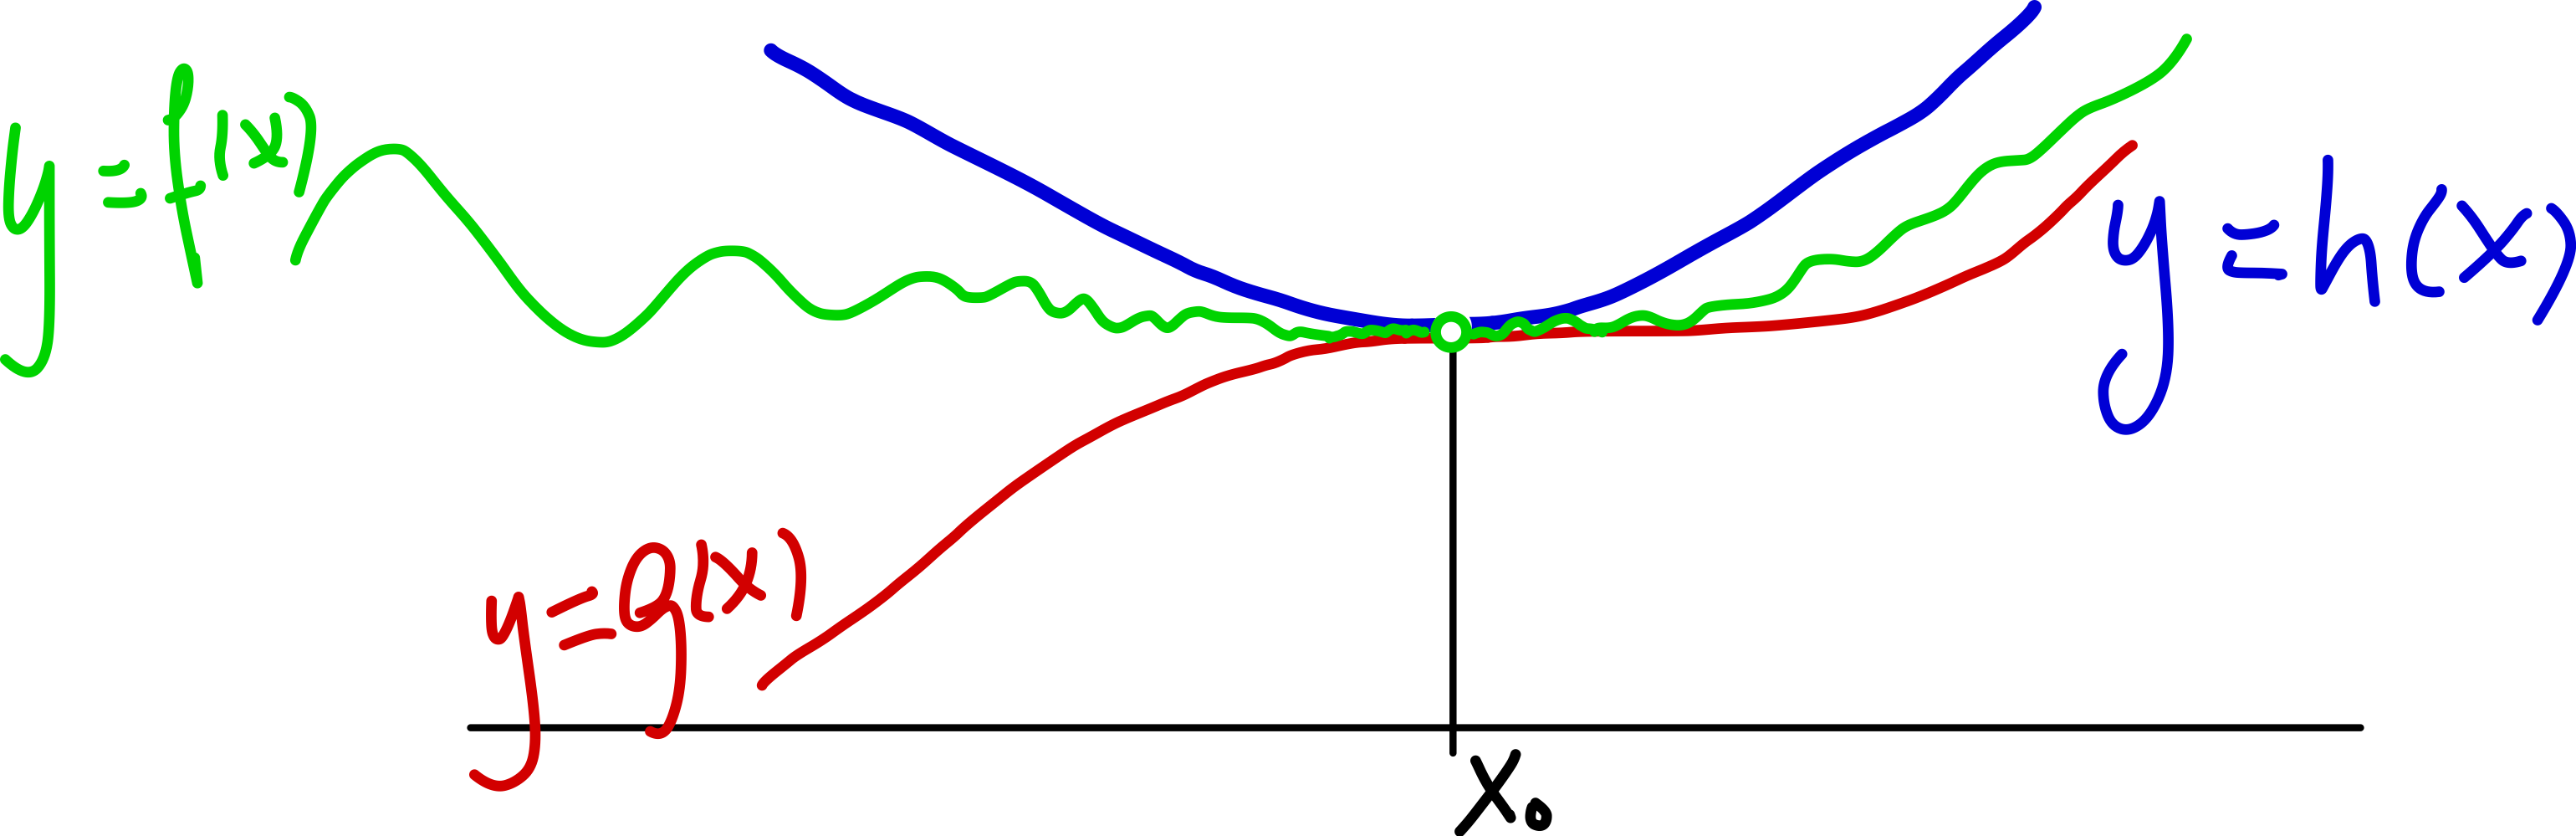
\includegraphics[width=.8\textwidth]{pics/emparedado.png}}


\begin{proposition}
    Sean $f$ y $g$ dos funciones tales que
    \[
    \lim_{x\to x_0} f(x)=\ell_1,
    \qquad
    \lim_{x\to x_0} g(x)=\ell_2.
    \]
    Entonces
    \begin{itemize}
        \item $\D \lim_{x\to x_0} \big( f(x) + g(x) \big) = \ell_1 + \ell_2$;
        \item $\D \lim_{x\to x_0} \big( f(x) \cdot g(x) \big) = \ell_1 \cdot \ell_2$;
        \item Si $\ell_2\neq 0$, $\D \lim_{x\to x_0} \frac{f(x)}{g(x)} = \frac{\ell_1}{\ell_2}$.
    \end{itemize}
\end{proposition}

\begin{example}
    Con estas nuevas reglas de cálculo, sabiendo que\footnote{Estos dos límites están para ser demostrados en los ejercicios.}
    \begin{itemize}
        \item $\D\lim_{x\to x_0} c=c$, para cualquier constante $c$.
        \item $\D\lim_{x\to x_0} x = x_0$, para cualquier $x_0\in\R$.
    \end{itemize}
    podemos ver que:
    \begin{itemize}
        \item $\D\lim_{x\to -1}  \big(3x+x^2\big) = -2$. En efecto
        \[ \lim_{x\to -1} 3x+ \lim_{x\to -1} x^2= 
        \lim_{x\to -1} 3 \cdot \lim_{x\to -1}x+ \lim_{x\to -1} x \cdot \lim_{x\to -1} x= 3\cdot(-1)+(-1)\cdot(-1)=-2.\]
        \item $\D\lim_{x\to 0} \frac{2x+1}{10+x^2}  = \frac{\lim_{x\to 0}(2x+1)}{\lim_{x\to 0}(10+x^2)}=\frac1{10}$ (porque el límite del denominador es no nulo).
        \item Si $p$ y $q$ son polinomios, entonces
        \[ 
        \D\lim_{x\to 1}  \frac{p(x)}{q(x)}  = \frac{\lim_{x\to 1}p(x)}{\lim_{x\to 1}q(x)} 
        =\frac{p(1)}{q(1)},\quad\text{si $q(1)\neq 0$.}
        \]
        
    \end{itemize}
\end{example}

\subsection{Más propiedades del límite}

\begin{theorem}[Teorema fundamental del límite]\label{T:TFL}
Sea $f$ una función definida en $(a,b)$ salvo quizás en $x_0\in(a,b)$.
Entonces 
\[ \D \limxo f(x)=\ell
\]
si y sólo si 
\begin{quote}
    para toda sucesión $\big(x_n\big)_{n\in\N}$ tal que $\D\lim_{n\to\infty} x_n = x_0$ (con $x_n\neq x_0$, para todo \niN) vale que $\lim_{n\to\infty}f(x_n)=\ell$.
\end{quote}
\end{theorem}

\begin{proof}
Supongamos primero que $\limxo f(x)=\ell$ y sea $\big(x_n\big)_{n\in\N}$ una sucesión tal que $\D\lim_{n\to\infty} x_n = x_0$ (con $x_n\neq x_0$, para todo \niN).
Sea $\epsilon>0$, entonces, como $\limxo f(x)=\ell$ existe $\delta>0$ tal que
\[
0<|x-x_0|<\delta\quad\implies\quad |f(x)-\ell|<\epsilon.
\]
Ahora bien, como $\D\lim_{n\to\infty} x_n = x_0$, para ese $\delta>0$, existe $N_0\in\N$ tal que
\[
|x_n-x_0|<\delta, \quad\text{para todo $n\ge N_0$}.
\]
Como además $x_n\neq x_0$, para todo \niN, resulta que 
\[
0<|x_n-x_0|<\delta, \quad\text{para todo $n\ge N_0$}.
\]
Luego, $\D |f(x_n)-\ell|<\epsilon, \quad\text{para todo $n\ge N_0$}$.

Hemos probado que dado $\epsilon>0$ existe $N_0\in\N$ tal que 
\[
|f(x_n)-\ell|<\epsilon, \quad\text{para todo $n\ge N_0$}.
\]
Es decir, $\D\lim_{n\to\infty}f(x_n) = \ell$.

Para probar la recíproca, supongamos que para toda sucesión $\big(x_n\big)_{n\in\N}$ tal que $\D\lim_{n\to\infty} x_n = x_0$ (con $x_n\neq x_0$, para todo \niN) vale que $\lim_{n\to\infty}f(x_n)=\ell$.
Debemos probar que $\D\limxo f(x)=\ell$.
Si esto no fuera cierto, entonces existiría $\epsilon>0$ tal que, cualquiera sea $\delta>0$, hay un $x$ que cumple $0<|x-x_0|<\delta$ y $|f(x)-\ell|\ge \epsilon$.
Entonces, tomamos, para cada $n\in\N$, $\delta=\frac1n$ y sea $x_n$ el correspondiente que cumple que $0<|x_n-x_0|<\frac1n$ y $|f(x_n)-\ell|\ge \epsilon$.
De esta manera, hemos construido una sucesión $\big(x_n\big)_{n\in\N}$ tal que $\D\lim_{n\to\infty} x_n = x_0$, con $x_n\neq x_0$, para todo \niN, para la cual no es cierto que $\lim_{n\to\infty}f(x_n)=\ell$. Esto contradice nuestra suposición, por lo que $\D\limxo f(x)=\ell$.
\end{proof}


\begin{example}
Con este teorema podemos conocer muchos más límites, por ejemplo:
\begin{itemize}
\item ?`$\D \lim_{x\to 25} \sqrt{x} $?
Veamos, si $\sucxn$ es una sucesión tal que $\lim_{n\to\infty} x_n = 25$, entonces $\D \lim_{n\to\infty} \sqrt{x_n} = \sqrt{25}=5$ por lo que hemos visto en el Capítulo~\ref{C:sucesiones}. Como esto se cumple para toda sucesión con límite igual a $25$, resulta que $\D \lim_{x\to 25} \sqrt{x} = 5$.
\end{itemize}
    
\end{example}

Este último teorema, más el trabajo hecho en el Capítulo~\ref{C:sucesiones} nos permite deducir en forma sencilla otras propiedades del límite:

\begin{proposition}
% Sean $f$ y $g$ funciones definidas en $(a,b)$ salvo quizás en $x_0\in(a,b)$.
Si se cumple que
\[
\limxo f(x)=\ell_1>0,
\qquad
\limxo g(x)=\ell_2,
\]
entonces
\begin{enumerate}[{\bf (a)}]
    \item $\D \limxo \big( \ln(f(x)) \big) = \ln (\ell_1)$.
    \item $\D \limxo f(x)^{g(x)} = \ell_1^{\ell_2}$.
\end{enumerate}
\end{proposition}

\begin{proof}
\begin{enumerate}[{\bf (a)}]
    \item Sea \sucxn una sucesión que tiende a $x_0$ ($x_n\neq x_0$, $\forall \niN$),
    entonces $f(x_n)$ tiende a $\ell_1$ por el Teorema~\ref{T:TFL}. 
    Luego, por la Proposición~\ref{P:logaritmo continuo}, 
    \[
    \lim_{n\to\infty} \big(\ln (f(x_n))\big) = \ln (\ell_1).
    \]
    Como esta conclusión vale para cualquier sucesión \sucxn que cumple la hipótesis, 
    resulta nuevamente por el Teorema~\ref{T:TFL} que $\D\limxo \big( \ln (f(x)) \big) = \ln (\ell_1)$.
    
    \item Sea \sucxn una sucesión que tiende a $x_0$ ($x_n\neq x_0$, $\forall \niN$),
    entonces $f(x_n)$ tiende a $\ell_1$ y $g(x_n)$ tiende a $\ell_2$ por el Teorema~\ref{T:TFL}. 
    Luego, por la Proposición~\ref{P:potencias continuas}, 
    \[
    \lim_{n\to\infty} f(x_n)^{g(x_n)} = \ell_1^{\ell_2}.
    \]
    Como esta conclusión vale para cualquier sucesión \sucxn que cumple la hipótesis, 
    resulta nuevamente por el Teorema~\ref{T:TFL} que $\D \limxo f(x)^{g(x)} = \ell_1^{\ell_2}$.\qedhere
\end{enumerate}
\end{proof}


\begin{example}
    Con este teorema podemos ver más ejemplos:
    \begin{itemize}
        \item $\D \lim_{x \to 8} \ln(4x-5) = \ln\big(\lim_{x\to 8} (4x-5)\big)=\ln (4\cdot 8-5) = \ln 27$.
        \item $\D \lim_{x \to 2} \ln \big( 2^{x+1} \big)
        = \ln \big( \lim_{x \to 2}  2^{x+1} \big)
        = \ln \big(   2^{\lim_{x \to 2} x+1} \big)
        = \ln \big(   2^{2+1} \big) = \ln 2^3 = 3 \ln 2
        $.
        \item $\D \lim_{x \to 2} (3x^2)^{4x+1} 
        = \big(\lim_{x \to 2}3x^2\big)^{\lim_{x \to 2}4x+1} 
        = (3\cdot2^2)^{4\cdot 2 + 1 }
        = 12^{9}
        $.
        \item $\D \lim_{x \to -3} \big(x^2+1\big)^x
        = \big(\lim_{x \to -3}x^2+1\big)^{\lim_{x \to -3}x}
        = \big((-3)^2+1\big)^{-3}
        = 10^{-3} = 0.001
        $.
    \end{itemize}
\end{example}


\begin{proposition}
    Sea $g$ una función %definida en $(a,b)$ salvo quizás en $x_0\in(a,b)$, y 
    tal que
    \[
    \limxo g(x) = y_0.
    \]
    Supongamos que $\lim_{y\to y_0}f(y)=f(y_0)$ (el límite de $f(y)$ cuando $y\to y_0$ existe y coincide con $f(y_0)$), entonces
    \[
    \limxo f\circ g(x) = f(y_0) = f(\limxo g(x)).
    \]
\end{proposition}

\begin{proof}
Sea \sucxn una sucesión que tiende a $x_0$ ($x_n\neq x_0$, $\forall \niN$), entonces 
\[
\lim_{n\to\infty} g(x_n) = y_0.
\]
Por lo tanto, la sucesión \sucyn dada por $y_n=g(x_n)$ es una sucesión que cumple $\D\lim_{n\to\infty}y_n=y_0$, 
y por el Teorema~\ref{T:TFL} resulta que $\D\lim_{n\to\infty}f(y_n)=f(y_0)$. Es decir
\[
\lim_{n\to\infty}f\circ g(x_n) = \lim_{n\to\infty}f(y_n)=f(y_0).
\]
Nuevamente, por el Teorema~\ref{T:TFL} resulta que $\D\limxo f\circ g(x) = f(y_0)$.
\end{proof}

\begin{example}
    Con este teorema podemos ver más ejemplos:
    \begin{itemize}
        \item $\D \lim_{x\to 4} \sgn(\underbrace{1-x}_{y})
        = \lim_{y\to -3} \sgn(y)=-1
        $,
        porque $\lim_{x\to4}y = -3$.
        \item $\D \lim_{x\to 0} \big(\underbrace{3x^2+8x+6}_{y\tox{0}6}\big)^7
        =\lim_{y\to 6} y^7 = 6^7
        $.
        \item $\D \lim_{x\to -1} \big(\underbrace{x+2}_{y\tox{-1}1}\big)^{1/5} 
        =\lim_{y\to 1} y^{1/5}=1^{1/5}=1
        $.
        \item $\D \lim_{x\to 3} \bigg[\ln\Big(\underbrace{\frac{x^2+3}{x-1}}_{y\tox{3}6}\Big)\bigg]^4
        =\lim_{y\to 6} \big[\underbrace{ \ln y}_{z\toy{6} \ln 6} ]^4
        = [\ln 6]^4
        $.
    \end{itemize}
\end{example}

\subsubsection*{Ejercicios de la sección~\getcurrentref{chapter}.\getcurrentref{section}}

\begin{enumerate}
\item Probar usando la definición que se cumplen las siguientes afirmaciones:

\begin{multicols}{2}
    \begin{enumerate}
        \item $\D \lim_{x\to 2} 3x-1=5 $.
        \item $\D \lim_{x\to 3} 4 x^2 = 36$.
        \item $\D \lim_{x\to 2} 3/x = 3/2$.
        \item $\D \lim_{x\to 1} x^2+2x = 3$.
    \end{enumerate}
\end{multicols}

\item Analizar la existencia de los siguientes límites:
\begin{multicols}{2}
    \begin{enumerate}
\item $\D \lim_{x\to 0} \sen \frac1x$;
\item $\D \lim_{x\to 0} \cos \frac1x$;
\item $\D \lim_{x\to 0} \sgn(x)$;
\item $\D \lim_{x\to 0} x \sen \frac1x$;
\item $\D \lim_{x\to 0} x^2 \sen \frac1x$;
\item $\D \lim_{x\to 0} (x + \sen \frac1x)$.
\end{enumerate}
\end{multicols}

\item ?`Para qué valores de $x_0\in\R$ existe $\limxo \lfloor x \rfloor$?

\item ?`Para qué valores de $x_0\in\R$ existe $\limxo \big(x - \lfloor x \rfloor\big)$?

\item Analizar la veracidad o falsedad de las siguientes afirmaciones:
\begin{enumerate}
    \item Si existe $\D\limxo \big(f(x)+g(x)\big)$, entonces existen
    $\D\limxo f(x)$ y $\D\limxo g(x)$.
    \item Si existe $\D\limxo \big(f(x)+g(x)\big)$ y existe
    $\D\limxo f(x)$, entonces existe $\D\limxo g(x)$.
    \item Si existe $\D\limxo \big(f(x)\cdot g(x)\big)$, entonces existen
    $\D\limxo f(x)$ y $\D\limxo g(x)$.
    \item Si existe $\D\limxo \big(f(x)\cdot g(x)\big)$ y existe
    $\D\limxo f(x)$, entonces existe $\D\limxo g(x)$.
    \item Si existe $\D\limxo \big(f(x)\cdot g(x)\big)$ y existe
    $\D\limxo f(x)\neq 0$, entonces existe $\D\limxo g(x)$.
    
\end{enumerate}

\item Sea $a>0$, $a\neq 1$ y supongamos que $\limxo f(x)=\ell>0$.
Demostrar que $\D\limxo \log_a(f(x)) = \log_a(\ell).$ (Recordar que $\D\log_a y = \frac{\ln y}{\ln a}$).

\item Consideremos la función constante $f(x)=a$, para algún $a\in\R$. Demostrar usando la definición que $\limxo f(x)=f(x_0)$, cualquiera sea $x_0\in\R$.
\item Consideremos la función \emph{identidad} $f(x)=x$. Demostrar usando la definición que $\limxo f(x)=f(x_0)$, cualquiera sea $x_0\in\R$.
\item Demostrar que si $a$ y $b$ son números reales, entonces la función lineal $f(x)=ax+b$ cumple que $\limxo f(x)=f(x_0)$, cualquiera sea $x_0\in\R$.
Usar lo demostrado en los ejercicios anteriores y las propiedades vistas en esta sección.
\item Demostrar que si $a$, $b$ y $c$ son números reales, entonces la función cuadrática $f(x)=ax^2+bx+c$ cumple que $\limxo f(x)=f(x_0)$, cualquiera sea $x_0\in\R$.
Usar lo demostrado en los ejercicios anteriores y las propiedades vistas en esta sección.
\item Demostrar que si $p(x)$ es una función polinomial, entonces $\limxo p(x)=p(x_0)$, cualquiera sea $x_0\in\R$.
\item Demostrar que si $p(x)$ y $q(x)$ son funciones polinomiales, entonces para la función racional $f(x)= \frac{p(x)}{q(x)}$ se cumple que $\limxo f(x)=f(x_0)$, cualquiera sea $x_0\in\R$, si $q(x_0)\neq0$.


\end{enumerate}


\section{Límites infinitos}

Ampliamos ahora el estudio del límite, considerando la posibilidad de que la variable $x$, o la función $f(x)$, o ambas, crezcan más allá de todo límite.

Comenzamos definiendo límites infinitos cuando $x$ tiende a un número real $x_0$.

\begin{definition}
    Sea $f$ una función definida en $(x_0,x_0+c)$ para algún $c>0$.
    Decimos que $f(x)$ tiende a $+\infty$ cuando $x$ tiende a $x_0$ por derecha, y escribimos
    \[
    \limxop f(x)=+\infty
    \]
    si se cumple lo siguiente:
    \begin{quote}
        Cualquiera sea $M>0$ existe $\delta>0$ tal que
        \[
        f(x)>M,\quad\text{para todo $x\in(x_0,x_0+\delta)$}.
        \]
    \end{quote}
\end{definition}

\begin{example}
    Veamos que 
    \[
    \lim_{x\to0^+} \frac1x = +\infty.
    \]
    Sea $M>0$, vemos que $\frac1x>M$ si y sólo si $0<x<\frac1M$. Por lo tanto, elegimos $\delta=\frac1M$ y se cumple que $\frac1x>M$ para todo $x\in(0,\delta)$.

    Hemos demostrado que dado $M>0$ existe $\delta>0$ tal que $\frac1x>M$ para todo $x\in(0,\delta)$.
    Luego $\D \lim_{x\to0^+} \frac1x = +\infty$.
\end{example}

Análogamente se define el límite infinito por izquierda.

\begin{definition}
    Sea $f$ una función definida en $(x_0-c,x_0)$ para algún $c>0$.
    Decimos que $f(x)$ tiende a $+\infty$ cuando $x$ tiende a $x_0$ por izquierda, y escribimos
    \[
    \limxom f(x)=+\infty
    \]
    si se cumple lo siguiente:
    \begin{quote}
        Cualquiera sea $M>0$ existe $\delta>0$ tal que
        \[
        f(x)>M,\quad\text{para todo $x\in(x_0-\delta,x_0)$}.
        \]
    \end{quote}
\end{definition}

\begin{example}
    Veamos que 
    \[
    \lim_{x\to0^-} \frac1{x^2} = +\infty.
    \]

    Sea $M>0$, vemos que $\frac1{x^2}>M$ si y sólo si $0<x^2<\frac1M$, o $\frac1M<\frac{1}{x^2}$. Por lo tanto, elegimos $\delta=\sqrt{\frac1M}$ y se cumple que $\frac1{x^2}>M$ para todo $x\in(-\delta,0)$.

    Hemos demostrado que dado $M>0$ existe $\delta>0$ tal que $\frac1{x^2}>M$ para todo $x\in(-\delta,0)$.
    Luego $\D \lim_{x\to0^-} \frac1{x^2} = +\infty$.
\end{example}

Ahora definimos los otros límites infinitos, como lo hicimos con sucesiones.

\begin{definition}
\begin{itemize}
    \item $\D\limxop f(x) = -\infty$ significa $\D\limxop \big(-f(x)\big)=+\infty$.
    \item $\D\limxom f(x) = -\infty$ significa $\D\limxom \big(-f(x)\big)=+\infty$.
    \item $\D\limxop f(x) = \infty$ significa $\D\limxop \big|f(x)\big|=+\infty$.
    \item $\D\limxom f(x) = \infty$ significa $\D\limxom \big|f(x)\big|=+\infty$.
\end{itemize}
\end{definition}

\begin{example}
    Veamos un ejemplo. Afirmamos que
    \[
    \lim_{x\to 0^+} \ln x = -\infty.
    \]
    Esto significa que $\lim_{x\to 0^+} \big(-\ln x\big) = +\infty$. Es decir, dado $M>0$ existe $\delta>0$ tal que vale la siguiente implicación
    \[
    0<x<\delta \quad\implies\quad -\ln x > M.
    \]
    Sea entonces $M>0$, consideremos $\delta = e^{-M}$. Si $0<x<\delta$, como $\ln$ es creciente, entonces $\ln x<\ln \delta = \ln e^{-M} = -M$, por lo tanto
    \[
    -\ln x > M.
    \]
    Hemos demostrado que dado $M>0$ existe $\delta>0$ tal que $-\ln x > M$ para todo $x\in (0,\delta)$. Es decir, $\lim_{x\to 0^+} \big(-\ln x\big) = +\infty$ que equivale a $\lim_{x\to 0^+}\ln x=-\infty$.
\end{example}

Nos falta considerar el caso en que la variable $x$ tiende a infinito.

\begin{definition}
    Sea $f$ definida en todos los puntos de un intervalo $(a,+\infty)$. Entonces
    \begin{itemize}
        \item Se dice que $\D\lim_{x\to +\infty} f(x) = \ell$ si, dado $\epsilon>0$ existe $K>0$ tal que 
        \[
        |f(x)-\ell|<\epsilon,
        \qquad\text{para todo $x>K$}.
        \]
        \item Se dice que $\D\lim_{x\to +\infty} f(x) = +\infty$ si, dado $M>0$ existe $K>0$ tal que 
        \[
        f(x)>M,
        \qquad\text{para todo $x>K$}.
        \]
        \item $\D\lim_{x\to +\infty} f(x) = -\infty$ significa que $\D\lim_{x\to +\infty}\big(- f(x)\big) = +\infty$
        \item $\D\lim_{x\to +\infty} f(x) = \infty$ significa que $\D\lim_{x\to +\infty}\big|f(x)\big| = +\infty$
    \end{itemize}
\end{definition}


\begin{example}
    Veamos que, si $\alpha>0$
    \[
    \lim_{x\to+\infty} x^{-\alpha} = 0.
    \]
    Sea $\epsilon>0$, observamos que para $x>0$, resulta
    \[
    0<x^{-\alpha}<\epsilon
    \quad\iff\quad
    0<\frac{1}{x^{\alpha}}<\epsilon
    \quad\iff\quad
    \frac1\epsilon<x^\alpha
    \quad\iff\quad
    \frac1{\epsilon^{1/\alpha}}<x.
    \]
    Elegimos entonces $K=1/{\epsilon^{1/\alpha}}$ y llegamos a que
    \[
    0< x^{-\alpha } < \epsilon, \qquad\text{para todo $x>K$},
    \]
    que a su vez implica que
    \[
    |x^{-\alpha } - 0| < \epsilon, \qquad\text{para todo $x>K$},
    \]
    Como $\epsilon>0$ era arbitrario, resulta que $\D\lim_{x\to+\infty} x^{-\alpha} = 0$.
\end{example}


\begin{example}
    Veamos que, si $\alpha>0$
    \[
    \lim_{x\to+\infty} x^{\alpha} = +\infty.
    \]
    Sea $M>0$, observamos que 
    \[
    x^\alpha > M
    \quad\iff\quad
    x > M^{1/\alpha}.
    \]
    Luego, elegimos $K = M^{1/\alpha}$ y resulta que 
    \[
    x^{-\alpha } > M, \qquad\text{para todo $x>K$}.
    \]
    Como $M>0$ era arbitrario, resulta que $\D\lim_{x\to+\infty} x^{\alpha} = +\infty$.
\end{example}

\begin{example}
    Veamos un ejemplo más. Afirmamos que 
    \[
    \lim_{x\to+\infty} \ln x = +\infty.
    \]
    Sea $M>0$, tomemos $K=e^M$, entonces, como la función $\ln$ es estrictamente creciente, resulta que, si $x>K$
    \[
    \ln x > \ln K = \ln e^M = M.
    \]
    Hemos demostrado que dado $M>0$ existe $K>0$ tal que 
    \[
    \ln x > M, 
        \qquad\text{para todo $x>K$}.
    \]
    Es decir, $\D\lim_{x\to+\infty} \ln x = +\infty$.
\end{example}

\begin{example}
    Consideremos ahora la función exponencial. Afirmamos que si $a>1$ entonces
    \[
    \lim_{x\to+\infty} a^x = +\infty.
    \]
    Sea $M>0$, tomemos $K=\max\{\log_a M, 1\}$ (si $M<1$ resulta $\log_a M<0$). Como $a>1$, la función $x\to a^x$ es estrictamente creciente, y entonces, si $x>K$ resulta que,
    \[
    a^x > a^K \ge a^{\log_a K} = K.
    \]
    Hemos demostrado que dado $M>0$ existe $K>0$ tal que 
    \[
    a^x > M, 
        \qquad\text{para todo $x>K$}.
    \]
    Es decir, $\lim_{x\to+\infty} a^x = +\infty$.
\end{example}

Presentamos ahora las últimas definiciones de límites cuando la variable independiente $x$ tiende a infinito.
\begin{definition}
    Sea $f$ definida en todos los puntos de un intervalo $(-\infty,a)$. Entonces
    \begin{itemize}
        \item Se dice que $\D\lim_{x\to -\infty} f(x) = \ell$ si, dado $\epsilon>0$ existe $K>0$ tal que 
        \[
        |f(x)-\ell|<\epsilon,
        \qquad\text{para todo $x<-K$}.
        \]
        \item Se dice que $\D\lim_{x\to -\infty} f(x) = +\infty$ si, dado $M>0$ existe $K>0$ tal que 
        \[
        f(x)>M,
        \qquad\text{para todo $x<-K$}.
        \]
        \item $\D\lim_{x\to -\infty} f(x) = -\infty$ significa que $\D\lim_{x\to -\infty}\big(- f(x)\big) = +\infty$
        \item $\D\lim_{x\to -\infty} f(x) = \infty$ significa que $\D\lim_{x\to -\infty}\big|f(x)\big| = +\infty$
    \end{itemize}
\end{definition}

\begin{example}
    Veamos que, si $n\in\N$
    \[
    \lim_{x\to-\infty} x^{-n} = 0.
    \]
    Sea $\epsilon>0$, observamos que para $x<0$, resulta
    \[
    |x^{-n}-0|<\epsilon
    \quad\iff\quad
    0<\frac{1}{|x|^n}<\epsilon
    \quad\iff\quad
    \frac1\epsilon<|x|^n
    \quad\iff\quad
    \frac1{\epsilon^{1/n}}<|x|.
    \]
    Elegimos entonces $K=1/{\epsilon^{1/n}}$ y llegamos a que
    \[
    | x^{-n} - 0| < \epsilon, 
    \qquad\text{para todo $x<-K$},
    \]
    Como $\epsilon>0$ era arbitrario, resulta que $\D\lim_{x\to-\infty} x^{-n} = 0$.
\end{example}

\begin{example}
    Veamos que, si $n\in\N$
    \[
    \lim_{x\to-\infty} x^{n} = \begin{cases} 
    +\infty, \quad&\text{si $n$ es par,}\\
    -\infty, \quad&\text{si $n$ es impar.}
    \end{cases}
    \]
    Consideremos el caso de $n$ impar.
    Tenemos que ver que $\D\lim_{x\to-\infty} -x^{n} = +\infty$.
    Pero si $n$ es impar $-x^n = (-x)^n$. Para $x<0$ tenemos que $(-x)^n=|x|^n$.
    Ahora bien 
    \[
    (-x)^n > M 
    \quad\iff\quad
    (-x) > M^{1/n}
    \quad\iff\quad
    x < - M^{1/n}.
    \]
    Elegimos $K = M^{1/n}$ y resulta que 
    \[
    (-x)^n > M ,
    \qquad\text{para todo $x<-K$}.
    \]
    Como $K>0$ era arbitrario, resulta que $\D\lim_{x\to-\infty} -x^{n} = +\infty$, o lo que es lo mismo $\D\lim_{x\to-\infty} x^{n} = -\infty.$
\end{example}

\begin{example}
    Consideremos nuevamente la función exponencial. Afirmamos que si $a>1$ entonces
    \[
    \lim_{x\to-\infty} a^x = 0.
    \]
    Sea $\epsilon>0$, tomemos $K=\max\{-\log_a \epsilon, 1\}$ (si $\epsilon>1$ resulta $\log_a \epsilon>0$). Como $a>1$, la función $x\to a^x$ es estrictamente creciente, y entonces, si $x<-K$ resulta que,
    \[
    0< a^x < a^{-K} \le a^{\log_a \epsilon} = \epsilon,
    \]
    que implica
    \[
    |a^x-0| < \epsilon.
    \]
    
    Hemos demostrado que dado $M>0$ existe $K>0$ tal que 
    \[
    |a^x-0| < \epsilon.
        \qquad\text{para todo $x<-K$}.
    \]
    Es decir, $\lim_{x\to-\infty} a^x = 0$.
\end{example}

Para todos los límites que hemos visto se cumplen las propiedades siguientes con demostraciones análogas a las que ya hemos visto:

\begin{itemize}
    \item Si $\D \lim f(x) = \ell_1$ y $\D \lim g(x)=\ell_2$, entonces:
    \begin{itemize}
        \item $\D \lim \big(f(x)+g(x)\big) = \ell_1+\ell_2$.
        \item $\D \lim \big(f(x)\cdot g(x)\big) = \ell_1\cdot \ell_2$.
        \item $\D \lim \big(f(x)/g(x)\big) = \ell_1/\ell_2$, si $\ell_2\neq 0$.
        \item $\D \lim \big(f(x)/g(x)\big) = \infty$, si $\ell_2= 0$ y $\ell_1\neq 0$.
        \item $\D \lim f(x)^{g(x)} = \ell_1^{\ell_2}$, si $\ell_1>0$.
    \end{itemize}
    \item Si $\D \lim f(x) = \ell$ y $\D \lim g(x)=+\infty$, entonces:
    \begin{itemize}
        \item $\D \lim \big(f(x)+g(x)\big) = +\infty$.
        \item $\D \lim \big(f(x)\cdot g(x)\big) = \begin{cases}
            +\infty, \quad&\text{si }\ell>0,\\
            -\infty, \quad&\text{si }\ell<0,\\
            \text{indeterminado}, \quad&\text{si }\ell=0.
        \end{cases}$
        \item $\D \lim \big(f(x)/g(x)\big) = 0$.
        \item $\D \lim f(x)^{g(x)} =\begin{cases}
            +\infty, \quad&\text{si }\ell>1,\\
            0, \quad&\text{si } 0<\ell<1,\\
            0, \quad&\text{si } \ell=0 \text{ y }f(x)\ge 0.
        \end{cases}$
    \end{itemize}
    \item Si $\D \lim f(x) = \ell$ y $\D \lim g(x)=-\infty$, entonces:
    \begin{itemize}
        \item $\D \lim \big(f(x)+g(x)\big) = -\infty$.
        \item $\D \lim \big(f(x)\cdot g(x)\big) = \begin{cases}
            -\infty, \quad&\text{si }\ell>0,\\
            +\infty, \quad&\text{si }\ell<0,\\
            \text{indeterminado}, \quad&\text{si }\ell=0.
        \end{cases}$
        \item $\D \lim \big(f(x)/g(x)\big) = 0$.
        \item $\D \lim f(x)^{g(x)} =\begin{cases}
            0, \quad&\text{si }\ell>1,\\
            +\infty, \quad&\text{si } 0<\ell<1,\\
            +\infty, \quad&\text{si } \ell=0 \text{ y }f(x)\ge 0.
        \end{cases}$
    \end{itemize}
\end{itemize}

\begin{proposition}
    Si $\D\limxo g(x) = +\infty$ y $\D\lim_{y\to+\infty}f(y)=\ell$, entonces $\D\limxo f\circ g(x) = \ell$.
\end{proposition}

\begin{proof}
Sea $\epsilon>0$. Como $\D\lim_{y\to+\infty}f(y)=\ell$, existe $K>0$ tal que
\[
|f(y)-\ell|<\epsilon,
\qquad\text{para todo $y>K$}.
\]
Ahora bien, como $\D\limxo g(x) = +\infty$, existe $\delta>0$ tal que 
\[
0<|x-x_0|<\delta
\quad\implies\quad
g(x) > K.
\]
Por lo tanto, si $0<|x-x_0|<\delta$, resulta
\[
g(x)>K
\quad\implies\quad
|f(g(x))-\ell|<\epsilon
\quad\iff\quad
|f\circ g(x))-\ell|<\epsilon.
\]
Hemos demostrado que dado $\epsilon>0$ existe $\delta>0$ tal que
\[
|f\circ g(x))-\ell|<\epsilon,
\qquad\text{para todo $x\in(x_0-\delta,x_0+\delta)\setminus\{x_0\}$}.
\qedhere
\]
\end{proof}

\begin{example}
    Si definimos $f(y) = \Big(1+\frac1y\Big)^y$, sabemos que $\lim_{y\to+\infty}f(y)=e$.

    Si ahora $g(x)$ es una función que cumple que $\limxo g(x) = +\infty$, entonces
    \[
    \limxo f\circ g(x) = e.
    \]
    Es decir, 
    \[
    \limxo \D \Big(1+\frac{1}{g(x)}\Big)^{g(x)}=e.
    \]

    Lo mismo vale si en todos las fórmulas donde aparece $\limxo$, reemplazamos este límite por $\limxop$, o $\limxom$, o $\lim_{x\to+\infty}$ o $\lim_{x\to-\infty}$.

    Por ejemplo, $\lim_{x\to 0^+}\frac1x=+\infty$, entonces 
    \[
    \lim_{x\to 0^+} \Big(1+\frac{1}{\frac1x}\Big)^{1/x}
    =
    \lim_{x\to 0^+} \Big(1+x\Big)^{1/x} = e.
    \]
    Y también 
    \[
    \lim_{x\to 0^-} \Big(1+x\Big)^{1/x} = e,
    \]
    porque $\lim_{x\to 0^-}\frac1x=-\infty$.

    Por lo tanto, $\D\lim_{x\to 0} \Big(1+x\Big)^{1/x} = e.$
\end{example}

\begin{corollary}
    De manera análoga a la última proposición puede probarse lo siguiente, si $\D\lim_{y\to+\infty}f(y)=\ell$:
    \begin{itemize}
        \item Si $\D\limxop g(x) = +\infty$, entonces $\limxop f\circ g(x) = \ell$
        \item Si $\D\limxom g(x) = +\infty$, entonces $\limxom f\circ g(x) = \ell$
        \item Si $\D\lim_{x\to +\infty} g(x) = +\infty$, entonces $\lim_{x\to +\infty} f\circ g(x) = \ell$
        \item Si $\D\lim_{x\to -\infty} g(x) = +\infty$, entonces $\lim_{x\to -\infty} f\circ g(x) = \ell$
    \end{itemize}
\end{corollary}

\begin{corollary}
    De manera análoga a la última proposición puede probarse lo siguiente, si $\D\lim_{y\to+\infty}f(y)=+\infty$:
    \begin{itemize}
        \item Si $\D\limxop g(x) = +\infty$, entonces $\limxop f\circ g(x) = +\infty$
        \item Si $\D\limxom g(x) = +\infty$, entonces $\limxom f\circ g(x) = +\infty$
        \item Si $\D\lim_{x\to +\infty} g(x) = +\infty$, entonces $\lim_{x\to +\infty} f\circ g(x) = +\infty$
        \item Si $\D\lim_{x\to -\infty} g(x) = +\infty$, entonces $\lim_{x\to -\infty} f\circ g(x) = +\infty$
    \end{itemize}
\end{corollary}

\subsubsection*{Ejercicios de la sección~\getcurrentref{chapter}.\getcurrentref{section}}

\begin{enumerate}
\item Calcular los siguientes límites.
 Si el límite es infinito, indicar si es $+\infty$, $-\infty$ o meramente $\infty$.
   
\begin{multicols}{2}
    \begin{enumerate}
        \item $\D\lim_{x\to0} \frac{1}{x+x^2}$
        \item $\D\lim_{x\to0} \frac{1}{x^2+x^4}$
        \item $\D\lim_{x\to0} \frac{-1}{|x|}$
        \item $\D\lim_{x\to0^+} \frac{1}{\sqrt x}$
        \item $\D\lim_{x\to2} \frac{3}{(x-2)^2}$
        \item $\D\lim_{x\to0} \frac{x}{\sqrt{x^2+1}-1}$
    \end{enumerate}
\end{multicols}

\item Escribir proposiciones que relacionen todas las definiciones de límites de la Sección~\getcurrentref{chapter}.\getcurrentref{section} con límites de sucesiones.

\item Analizar la existencia de los siguientes límites:
   
\begin{multicols}{2}
    \begin{enumerate}
        \item $\D\lim_{x\to+\infty} \sen(x)$
        \item $\D\lim_{x\to+\infty} \cos(x)$
        \item $\D\lim_{x\to+\infty} \frac{\sen(x)}x$
        \item $\D\lim_{x\to+\infty} x\sen\Big(\frac\pi x\Big)$
        \item $\D\lim_{x\to0} \frac{|x|-x}{|x|+x}$
        \item $\D\lim_{x\to0} x\cdot\lfloor x \rfloor$
        \item $\D\lim_{x\to0} x\cdot\bigg\lfloor \frac1x \bigg\rfloor$
    \end{enumerate}
\end{multicols}

\item Calcular los siguientes límites.
 Si el límite es infinito, indicar si es $+\infty$, $-\infty$ o meramente $\infty$.
   
\begin{multicols}{2}
    \begin{enumerate}
    \item $\D \lim_{x\to+\infty} \frac{x^3+2x-1}{2x^3-3x+4}$
    \item $\D \lim_{x\to-\infty} \frac{x^3+2x-1}{2x^3-3x+4}$
    \item $\D \lim_{x\to+\infty} \frac{2x^2-3x}{x^3+1}$
    \item $\D \lim_{x\to-\infty} \frac{2x^2-3x}{x^3+1}$
    \item $\D \lim_{x\to+\infty} \frac{\sqrt{x^2+x+1}+\sqrt{x^2-x+1}}{x+\sqrt{x^2+1}}$
    \item $\D \lim_{x\to-\infty} \frac{\sqrt{x^2+x+1}+\sqrt{x^2-x+1}}{x+\sqrt{x^2+1}}$
    \item $\D \lim_{x\to+\infty} \frac{2+x^{5/3}}{3x+x^{1/5}}$
    \item $\D \lim_{x\to-\infty} \frac{2+x^{5/3}}{3x+x^{1/5}}$
    \item $\D \lim_{x\to+\infty} \frac{\sqrt{x}+x^{3/4}}{x^{1/3}+x^{2/3}}$
    \item $\D \lim_{x\to-\infty} \frac{x^2-1}{x+2}-\frac{x^2+1}{x+2}$
    \item $\D \lim_{x\to+\infty} \frac{\sqrt{x+1}-\sqrt{x-1}}{\sqrt{x+1}+\sqrt{x-1}}$
    \item $\D \lim_{x\to+\infty} x^2-2x$
    \item $\D \lim_{x\to+\infty} 2x^2+6x$
    \item $\D \lim_{x\to+\infty} \frac{\sqrt{x+\sqrt{x}}}{\sqrt{x+\sqrt{x+\sqrt{x}}}}$
    \item $\D \lim_{x\to+\infty} x\big(x-\sqrt{2x^2+3}\big)$
    \item $\D \lim_{x\to+\infty} \sqrt{x^2+2x}-x$
    \item $\D \lim_{x\to+\infty} x+\sqrt{1-x^3}$
    \item $\D \lim_{x\to+\infty} \bigg(\frac{x+1}{x+2}\bigg)^{2x}$
    \item $\D \lim_{x\to+\infty} \bigg(\frac{2x^2+5}{x^2+1}\bigg)^{3x^2+1}$
    \item $\D \lim_{x\to+\infty} \bigg(\frac{x+4}{x+6}\bigg)^{x^2}$
    \item $\D \lim_{x\to+\infty} \bigg(\frac{x^2+1}{x^2+2}\bigg)^{x^3}$
    
    
    \end{enumerate}
\end{multicols}


\end{enumerate}


\section{La notación \texorpdfstring{$o(h)$}{o(h)}}

\begin{definition}
    Sea $f$ una función real definida en $(-c,c)$, salvo quizás en $x=0$, para algún $c>0$. Se dice que $f(h)$ es una \emph{$o$ (chiquita) de $h$ cuando $h$ tiende a cero} y se escribe $f(h)=o(h)$ si
    \[
    \lim_{h\to 0} \frac{f(h)}{h} = 0.
    \]
    Es decir, $f(h) = o(h)$ si \emph{$f(h)$ tiende a cero más rápido que $h$}, cuando $h$ tiende a cero.
\end{definition}

Antes de ver algunos ejemplos, observemos que:
\[
\lim_{h\to 0} \frac{f(h)}{h} = 0
\quad\iff\quad
\lim_{h\to 0} \frac{|f(h)|}{|h|} = 0.
\]

\begin{example} Veamos algunos ejemplos:
\begin{itemize}
    \item Si $f(x) = x^2$, entonces $f(h) = o(h)$.
    En efecto, para $h\neq 0$
    \[
    \frac{f(h)}h = \frac{h^2}{h} = h \to 0 \quad\text{cuando $h\to0$}.
    \]
    % \item Si $f(x) = x^3$, entonces $f(h) = o(h)$.
    \item Si $f(x) = |x|^{1.1}$, entonces $f(h) = o(h)$.
    En efecto, para $h\neq 0$
    \[
    \frac{|f(h)|}{|h|} = \frac{|h|^{1.1}}{|h|} = |h|^{0.1} \to 0 \quad\text{cuando $h\to0$}.
    \]
    % \item Si $f(x) = |x|^\alpha$ y $\alpha > 1$, entonces $f(h) = o(h)$.
    % \item Si $f(x) = \frac{x}{\log x}$, entonces $f(h) = o(h)$.
    % \item Si $f(x) = 1-\cos(x)$, entonces $f(h) = o(h)$.
    % \item Si $f(x) = |x|$, entonces $f(h) \neq o(h)$.
    \item Si $f(x) = \sqrt{|x|}$, entonces $f(h) \neq o(h)$.
    En efecto, para $h\neq 0$
    \[
     \frac{|f(h)|}{|h|} = \frac{\sqrt{|h|}}{|h|} = \frac1{\sqrt{|h|}} \not\to 0 \quad\text{cuando $h\to0$}.
    \]
    % \item Si $f(x) = 1$, entonces $f(h) \neq o(h)$.
    % \item Si $f(x) = |x|^\alpha$ y $\alpha \le 1$, entonces $f(h) \neq o(h)$.
    % \item Si $f(x) = \log(|x|)$, entonces $f(h) \neq o(h)$.
    % \item Si $f(x) = \sen(x)$, entonces $f(h) \neq o(h)$.
\end{itemize}
\end{example}

\begin{lemma}
  Si $f(h)=o(h)$, entonces $\lim_{h\to0}f(h) = 0$.
\end{lemma}

\begin{proof}
    Observamos que, para $h\neq 0$,
    \[
    f(h) = \frac{f(h)}{h} \cdot h .
    \]
    Como $f(h)=o(h)$ resulta que $\lim_{h\to0} \frac{f(h)}{h} = 0$, y obviamente $\lim_{h\to0}h=0$.
    Por lo tanto, por la regla del límite del producto, $\lim_{h\to0}f(h)=0$.
\end{proof}

\begin{remark}
    No es cierto que si $\lim_{h\to0}f(h) = 0$, entonces $f(h) = o(h)$.
    Por ejemplo, la función $f(x) = x$ cumple que $\lim_{h\to0}f(h) = 0$ y sin embargo, $f(h) \neq o(h)$, porque
    \[
    \frac{f(h)}{h} = \frac hh = 1 \not\to 0, \text{ cuando $h\to 0$}.
    \]
\end{remark}


Es fácil deducir las siguientes propiedades.

\begin{theorem}[Propiedades]
    \begin{enumerate}[{\bf(a)}]
        \item Si $f(h)=o(h)$, entonces $cf(h) = o(h)$.
        \item Si $f(h)=o(h)$ y $g(h) = o(h)$, entonces $f(h)+g(h) = o(h)$.
        \item Si $f(h)=o(h)$ y $g(h) = o(h)$, entonces $f(h)g(h) = o(h)$.
    \end{enumerate}
\end{theorem}


\begin{theorem}
Si $f(h)=o(h)$, $f(0)=0$, y $g$ es una función real que cumple
$|g(h)| \le C|h|$, para todo $|h|<p$, para algún $p>0$ y $C>0$, entonces $f\circ g(h) = o(h)$.
\end{theorem}

\begin{proof}
    Tenemos que demostrar que $\lim_{h\to0} \frac{f\circ g(h)}{h} = 0$.
    Observemos que
    \[
    \text{Si $h \neq 0$}, \quad
    \frac{f\circ g(h)}{h} = \begin{cases}
        0,\quad&\text{si }g(h) = 0,\\
        \frac{f(g(h))}{g(h)} \frac{g(h)}{h}, \quad&\text{si }g(h) \neq 0.
    \end{cases}
    \]
    Sea ahora $\eps > 0$. Como $f(H)=o(H)$, existe $\eta > 0$ tal que
    \[
    \left| \frac{f(H)}{H} \right| \le \frac{\eps}{C}, \quad\text{para todo } H \in (-\eta,\eta) .
    \]
    Si ahora elegimos $\delta = \min\{\eta,p\}$ resulta que
    \[
    \left| \frac{f\circ g(h)}{h} \right| < \frac{\eps}C = \eps, \quad\text{para todo }h \in (-\delta,\delta).
    \]
    Hemos demostrado que dado $\eps > 0$ existe $\delta > 0$ tal que
    \[
    \left| \frac{f\circ g(h)}{h} - 0 \right| < \eps, \quad\text{para todo }h \in (-\delta,\delta).
    \]
    Es decir, $\lim_{h \to 0} \frac{f\circ g(h)}{h} = 0$, o lo que es lo mismo, $f\circ g(h) = o(h)$.
\end{proof}


\subsubsection*{Ejercicios de la sección~\getcurrentref{chapter}.\getcurrentref{section}}

\begin{enumerate}
\item Determinar cuáles de las siguientes funciones cumplen que $f(h)=o(h)$:
\begin{multicols}{2}
\begin{enumerate}
    % \item $f(x) = x^2$
    \item $f(x) = x^3$
    \item $f(x) = 1$
    \item $f(x) = |x|^{1.001}$
    \item $f(x) = |x|^\alpha$ con $\alpha > 1$
    \item $f(x) = |x|^{1/3}$
    \item $f(x) = |x|$
    \item $f(x) = |x|^\alpha$ con $\alpha \le 1$
    \item $f(x) = \frac{x}{\log |x|}$
    % \item $f(x) = 1-\cos(x)$
    \item $f(x) = \log(|x|)$
    \item $f(x) = e^x$
    \item $f(x) = e^{-1/|x|}$
    
    % \item $f(x) = \sen(x)$, 
\end{enumerate}    
\end{multicols}

\item Demostrar las siguientes afirmaciones:
    \begin{enumerate}
        \item Si $f(h)=o(h)$, entonces $cf(h) = o(h)$.
        \item Si $f(h)=o(h)$ y $g(h) = o(h)$, entonces $f(h)+g(h) = o(h)$.
        \item Si $f(h)=o(h)$ y $g(h) = o(h)$, entonces $f(h)g(h) = o(h)$.
    \end{enumerate}

\end{enumerate}

\section{Funciones continuas}

Vimos en la primera sección de este capítulo (en la Definición~\ref{D:continuidad}) que
una función $f(x)$ es continua en $x_0$ si se cumple lo siguiente:
    \begin{quote}
        Para cada $\epsilon > 0$, existe $\delta > 0$ tal que
        \[ 
        |f(x) - f(x_0)| < \epsilon,
        \]
        para todos los valores $x$ que cumplen $|x-x_0|<\delta$.
    \end{quote}

Luego vimos que $\lim_{x\to x_0} f(x) = \ell$ (Definición~\ref{D:limite}) si se cumple lo siguiente:
    \begin{quote}
        Para cada $\epsilon > 0$, existe $\delta > 0$ tal que
        \[ 
        |f(x) - \ell| < \epsilon,
        \]
        para todos los valores $x$ que cumplen $0<|x-x_0|<\delta$.
    \end{quote}

Analizando estas dos definiciones, vemos que
\[
f \text{ es continua en $x_0$}
\quad\text{si y sólo si}\quad
\limxo f(x) = f(x_0).
\]
Es decir, una función $f$ es continua en un punto $x_0$ si:
\begin{itemize}
    \item Existe (y es finito) $\D\limxo f(x)$;
    \item $f$ está definida en $x_0$, es decir, existe $f(x_0)$;
    \item El límite coincide con el valor de la función en ese punto: $\D\limxo f(x)=f(x_0)$.
\end{itemize}

Entonces hay tres condiciones que implican la \emph{discontinuidad} de una función $f$ en un punto $x_0$:

\begin{enumerate}
    \item Si no existe $\D\limxo f(x)$ (o es infinito).
    \begin{itemize}
        \item Para la función \emph{signo}:
        \[
         f(x) = \sgn(x)  = \begin{cases}
    -1, \quad &\text{si $x<0$},\\
    0, \quad &\text{si $x=0$},\\
    1, \quad &\text{si $x>0$},
    \end{cases}
    \]
    no existe $\lim_{x\to 0} f(x)$, dado que los límites por izquierda y por derecha no coinciden.
    Por lo tanto $f(x)$ no es continua en $x_0=0$.

    \item Para la función
    \[
    f(x) = \begin{cases}
    \sen\frac1x, \quad &\text{si $x\neq0$},\\
    0, \quad &\text{si $x=0$},
    \end{cases}
    \]
    tampoco existe $\lim_{x\to 0} f(x)$ (ya vimos esto en un ejercicio).
    Por lo tanto $f(x)$ no es continua en $x_0=0$.

    \item Para la función 
    \[
    f(x) = \begin{cases}
    \frac1x, \quad &\text{si $x\neq0$},\\
    0, \quad &\text{si $x=0$},
    \end{cases}
    \]
    se cumple que $\lim_{x\to0}f(x) = \infty$.
    Por lo tanto $f(x)$ no es continua en $x_0=0$.
    \end{itemize}

    \item Si $f$ no está definida en $x_0$.
    \begin{itemize}
        \item La función $\D f(x) = \frac{x^2-4}{x-2}$ no está definida en $x=2$.
        Por lo tanto no es continua en $x_0=2$.

        \item La función $\D f(x) = \frac{x}{|x|}$ no está definida en $x=0$.
        Por lo tanto no es continua en $x_0=0$.
    \end{itemize}

    \item Si existe $\D\limxo f(x)$ y está definida $f(x_0)$ pero no coinciden.
    \begin{itemize}
        \item  La función 
    \[
    f(x) = \begin{cases} x, \quad&\text{si $x\neq 3$}\\
    0, \quad&\text{si $x=3$},
    \end{cases}
    \]
    está definida en $x=3$, $f(3)=0$ y existe $\lim_{x\to3}f(x) = 3$, 
    pero $f(3)=0\neq \lim_{x\to3}f(x) = 3$.
        \item  La función 
    \[
    f(x) = \begin{cases} \frac{x^2-9}{x-3}, \quad&\text{si $x\neq 3$}\\
    10, \quad&\text{si $x=3$},
    \end{cases}
    \]
    está definida en $x=3$, $f(3)=10$ y existe $\lim_{x\to3}f(x) = 6$, 
    pero $f(3)=10\neq \lim_{x\to3}f(x) = 6$.
    \end{itemize}
\end{enumerate}



\paragraph{Clasificación de discontinuidades.}
Cuando una función no es continua en un punto $x_0$ decimos que \emph{es discontinua en $x_0$}.
Como hemos visto, hay diferentes \emph{tipos de discontinuidades}:
\begin{description}
    \item[Discontinuidad evitable:]
    Si existe $\D\limxo f(x)$ se dice que la discontinuidad es \emph{evitable} porque se puede definir $f(x_0)$ igual a ese límite, y entonces la función resulta continua en $x_0$.
    Por ejemplo, la función $\D f(x) = \frac{x^2-9}{x-3}$ tiene una discontinuidad evitable en $x=3$, porque $\lim_{x\to3}f(x) = 6$. Re-definiendo 
    \[
    f(x) = \begin{cases} \frac{x^2-9}{x-3}, \quad&\text{si $x\neq 3$}\\
    6, \quad&\text{si $x=3$},
    \end{cases}
    \]
    $f(x)$ resulta continua.

    \item[Discontinuidad de primera especie o de salto:]
Si existen $\D\limxop f(x)$ y $\D\limxom f(x)$ pero no coinciden se dice que la discontinuidad es \emph{de primera especie} o \emph{de salto}. Este es el caso de la función $\sgn(x)$ en $x_0=0$ o de la función $\lfloor x \rfloor$ en todo $x_0\in\Z$.

    \item[Discontinuidad de segunda especie:]
    Diremos que la discontinuidad es \emph{de segunda especie} en todos los otros casos.
    Es decir, cuando no exista alguno de los límites laterales, o cuando algún límite lateral sea infinito.
    Por ejemplo, la función $f(x) = \sen\frac1x$ tiene una discontinuidad de segunda especie en $x_0=0$ ya que no existen los límites laterales cuando $x\to 0$.
    La función $f(x) = \frac1x$ también tiene una discontinuidad de segunda especie en $x_0=0$, ya que $\lim_{x\to 0}\frac1x = \infty$.
        
    
\end{description}

Observamos ahora que hemos definido el concepto de que una función sea continua en un punto $x_0$ de un intervalo $(a,b)$ donde está definida la función. ?`Qué quiere decir que una función es continua en un intervalo $(a,b)$?


\begin{definition}[Continuidad en un intervalo]
Dada $f:(a,b)\to \R$, diremos que $f$ es continua en $(a,b)$ o simplemente \emph{continua} si $f$ es continua en $x_0$ para todo $x_0\in(a,b)$.
\end{definition}


\begin{proposition}
La función $\ln:(0,+\infty)\to\R$ es continua, y si $a>0$ la función exponencial $f:\R\to\R$ dada por $f(x) = a^x$ también es continua.
\end{proposition}

\begin{proof}
    Sea $x_0 \in (0,+\infty)$. Ya vimos que cualquiera sea la sucesión \sucxn que cumpla $\lim x_n = x_0$, resulta que $\lim \ln(x_n) = \ln(x_0)$.
    Luego, $\D\limxo \ln(x) = \ln(x_0)$. Por lo tanto, $\ln(x)$ es continua en $x_0$ para todo $x_0\in(0,+\infty)$.

    Sea $x_0\in\R$. 
    Ya vimos que cualquiera sea la sucesión \sucxn que cumpla $\lim x_n = x_0$, resulta que $\lim a^{x_n} = a^{x_0}$.
    Luego, $\D\limxo a^x = a^{x_0}$. Por lo tanto, la función exponencial $a^x$ es continua en $x_0$ para todo $x_0\in\R$.
\end{proof}

Como consecuencia del ejercicio~\ref{ej:polinomios-continuos} de la Sección~\ref{S:continuidad-propiedades} resulta lo siguiente:

\begin{proposition}
    Si $p$ es una función polinomial, entonces es continua en $\R$.

    Si $f$ es una función racional (cociente de dos polinomios), entonces es continua en todo punto donde no se anula el denominador.
\end{proposition}

\begin{proof}
    Ver ejercicio~\ref{ej:polinomios-continuos} de la Sección~\ref{S:continuidad-propiedades}.
\end{proof}

\begin{example}
    Veamos como ejemplo la continuidad de la función 
    \[
    f(x) = \begin{cases}
        \frac{x^2-4}{x-2} \quad&\text{si }x>2,\\
        3  \quad&\text{si }x=2,\\
        x^3-4  \quad&\text{si }x<2,
    \end{cases}
    \]
    Consideremos primero $x_0=2$. Para ver si existe $\lim_{x\to 2}f(x)$ analizamos los límites laterales.
    Por la derecha:
    \[
    \lim_{x\to 2^+} f(x) 
    = \lim_{x\to 2^+} \frac{x^2-4}{x-2} 
    = \lim_{x\to 2^+} \frac{(x-2)(x+2)}{x-2} 
    = \lim_{x\to 2^+} (x+2) = 4.
    \]
    Por la izquierda
    \[
    \lim_{x\to 2^-} f(x) 
    = \lim_{x\to 2^-} x^3-4
    = 2^3-4
    = 4.
    \]
    Como los límites laterales coinciden, $\lim_{x\to2}f(x) = 4$.
    Como $f(2) = 3\neq 4$, la función es discontinua en $x_0=2$, aunque la discontinuidad es \emph{evitable}.

    Si ahora tomamos $x_0<2$, vemos que $x_0 \in (-\infty,2)$.
    En este intervalo la función $f$ es polinomial y por lo tanto $\limxo f(x) = f(x_0)$.

    Si ahora tomamos $x_0>2$, vemos que $x_0 \in (2,+\infty)$.
    En este intervalo la función $f$ es racional y por lo tanto continua en $x_0$ porque el denominador no se anula en $x_0$. Entonces $\limxo f(x) = f(x_0)$.

    En conclusión, $f(x)$ es continua en $x_0$ para todo $x_0\neq 2$.
    Es discontinua en $x_0=2$ donde tiene una discontinuidad evitable.
\end{example}

\subsection{Funciones trigonométricas.}
Pasemos ahora a estudiar la continuidad de las funciones trigonométricas. Para ello, recordamos la definición:

\centerline{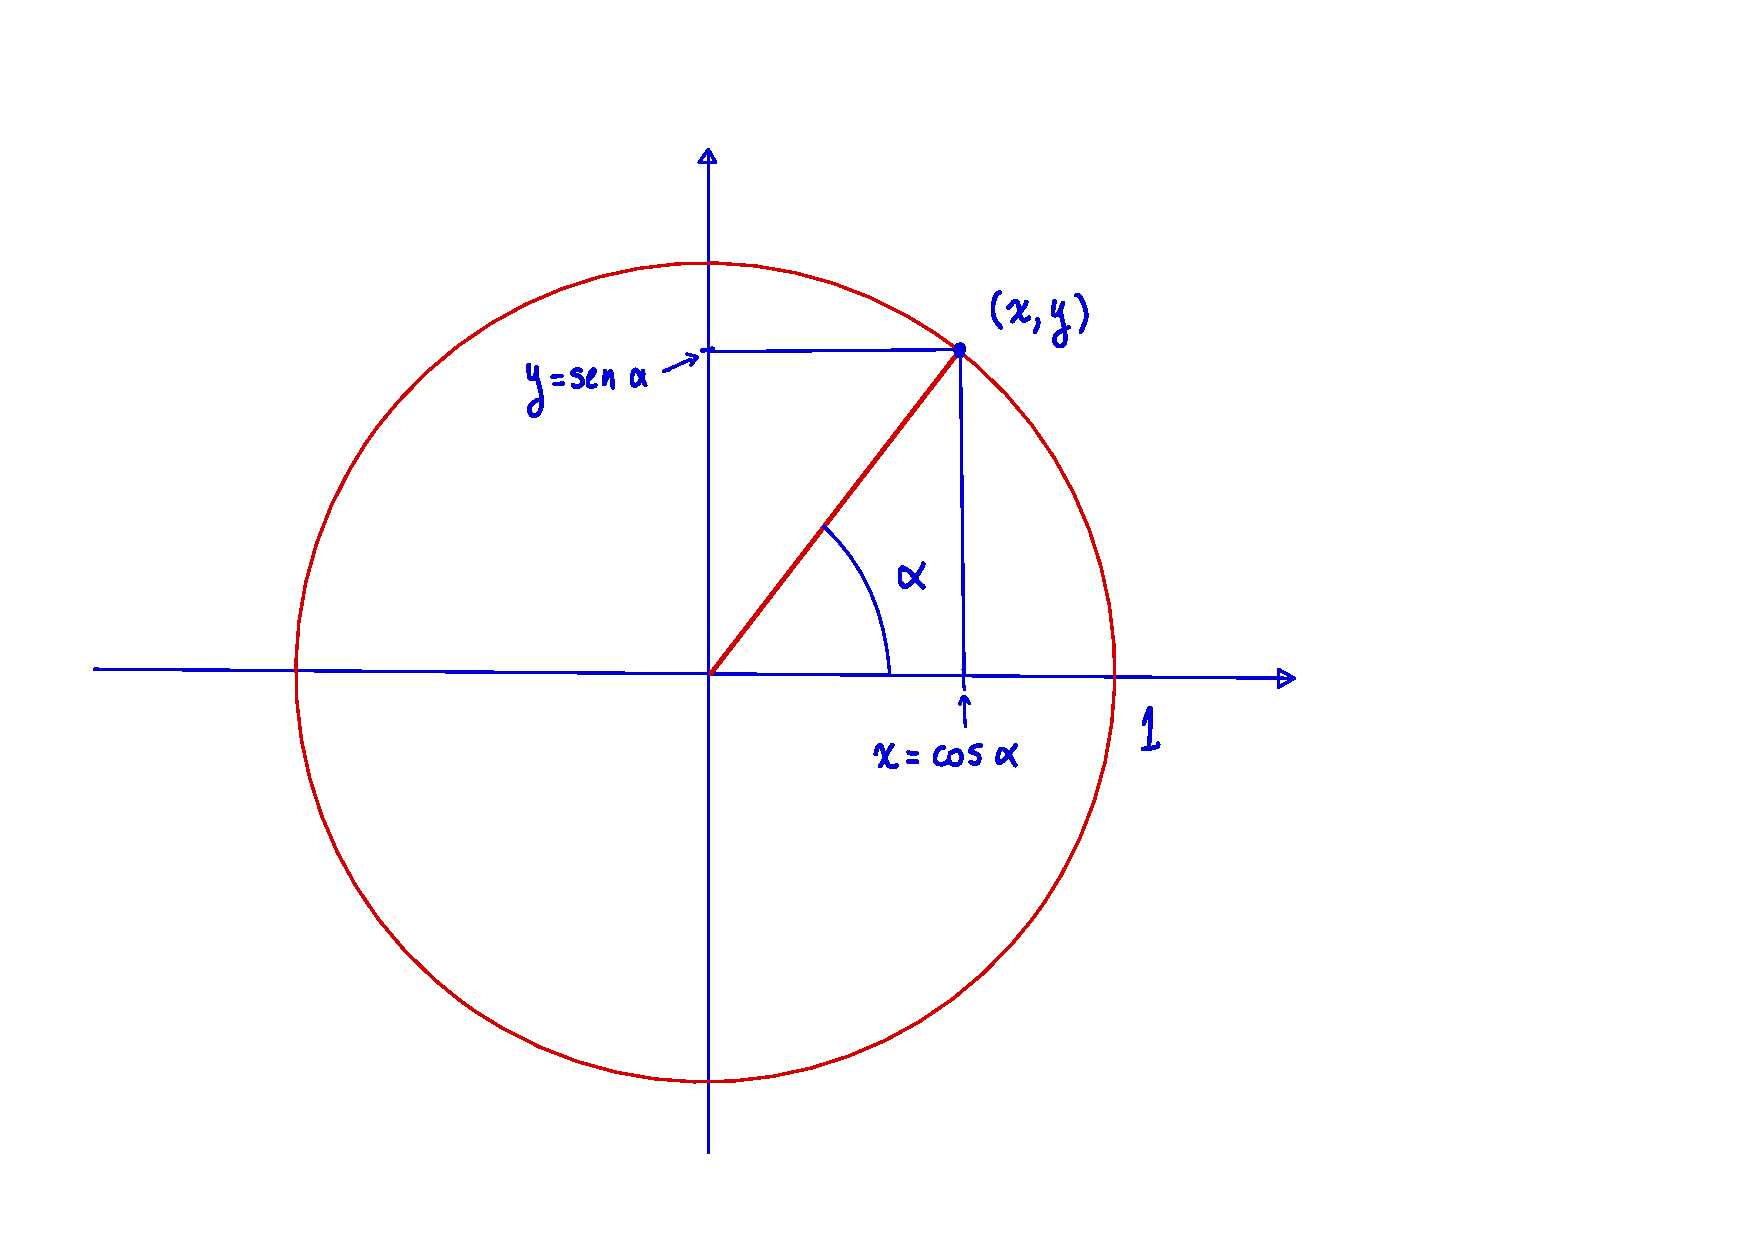
\includegraphics[width=.8\textwidth]{pics/trigonometricas.pdf}}

Dado un ángulo $\alpha\in\R$, giramos el segmento que une el origen de coordenadas con el punto $(1,0)$ un ángulo $\alpha$ alrededor del origen, en sentido positivo (antihorario) si $\alpha>0$ y negativo (horario) si $\alpha<0$. El punto $(1,0)$ va a parar a un punto $(x,y)$ de la circunferencia unitaria, es decir $x^2+y^2=1$. Definimos entonces las funciones 
\[
\cos\alpha=x,\qquad \sen\alpha=y,
\]
con dominio todo el conjunto de los reales.
Y a partir de estas, definimos las demás funciones trigonométricas:
\begin{align*}
    \tan \alpha &= \frac{\sen\alpha}{\cos\alpha}
    & \cotan\alpha &= \frac{\cos\alpha}{\sen\alpha}
    \\
    \sec\alpha&= \frac{1}{\cos\alpha}
    & \cosec\alpha &= \frac{1}{\sen\alpha}.
\end{align*}
El dominio de estas funciones es todo $\R$ excepto los puntos donde los denominadores de anulan.

Comenzamos ahora a estudiar la continuidad de la función $f(x)=\sen(x)$. Consideremos $x\in(-\pi/2,\pi/2)$. 
Cuando medimos el ángulo en radianes, la medida del ángulo en radianes $x$ coincide con la longitud del arco de circunferencia subtendido. Por lo tanto, para $0\le x<\pi/2$ resulta que $0\le \sen(x)\le x$.

\centerline{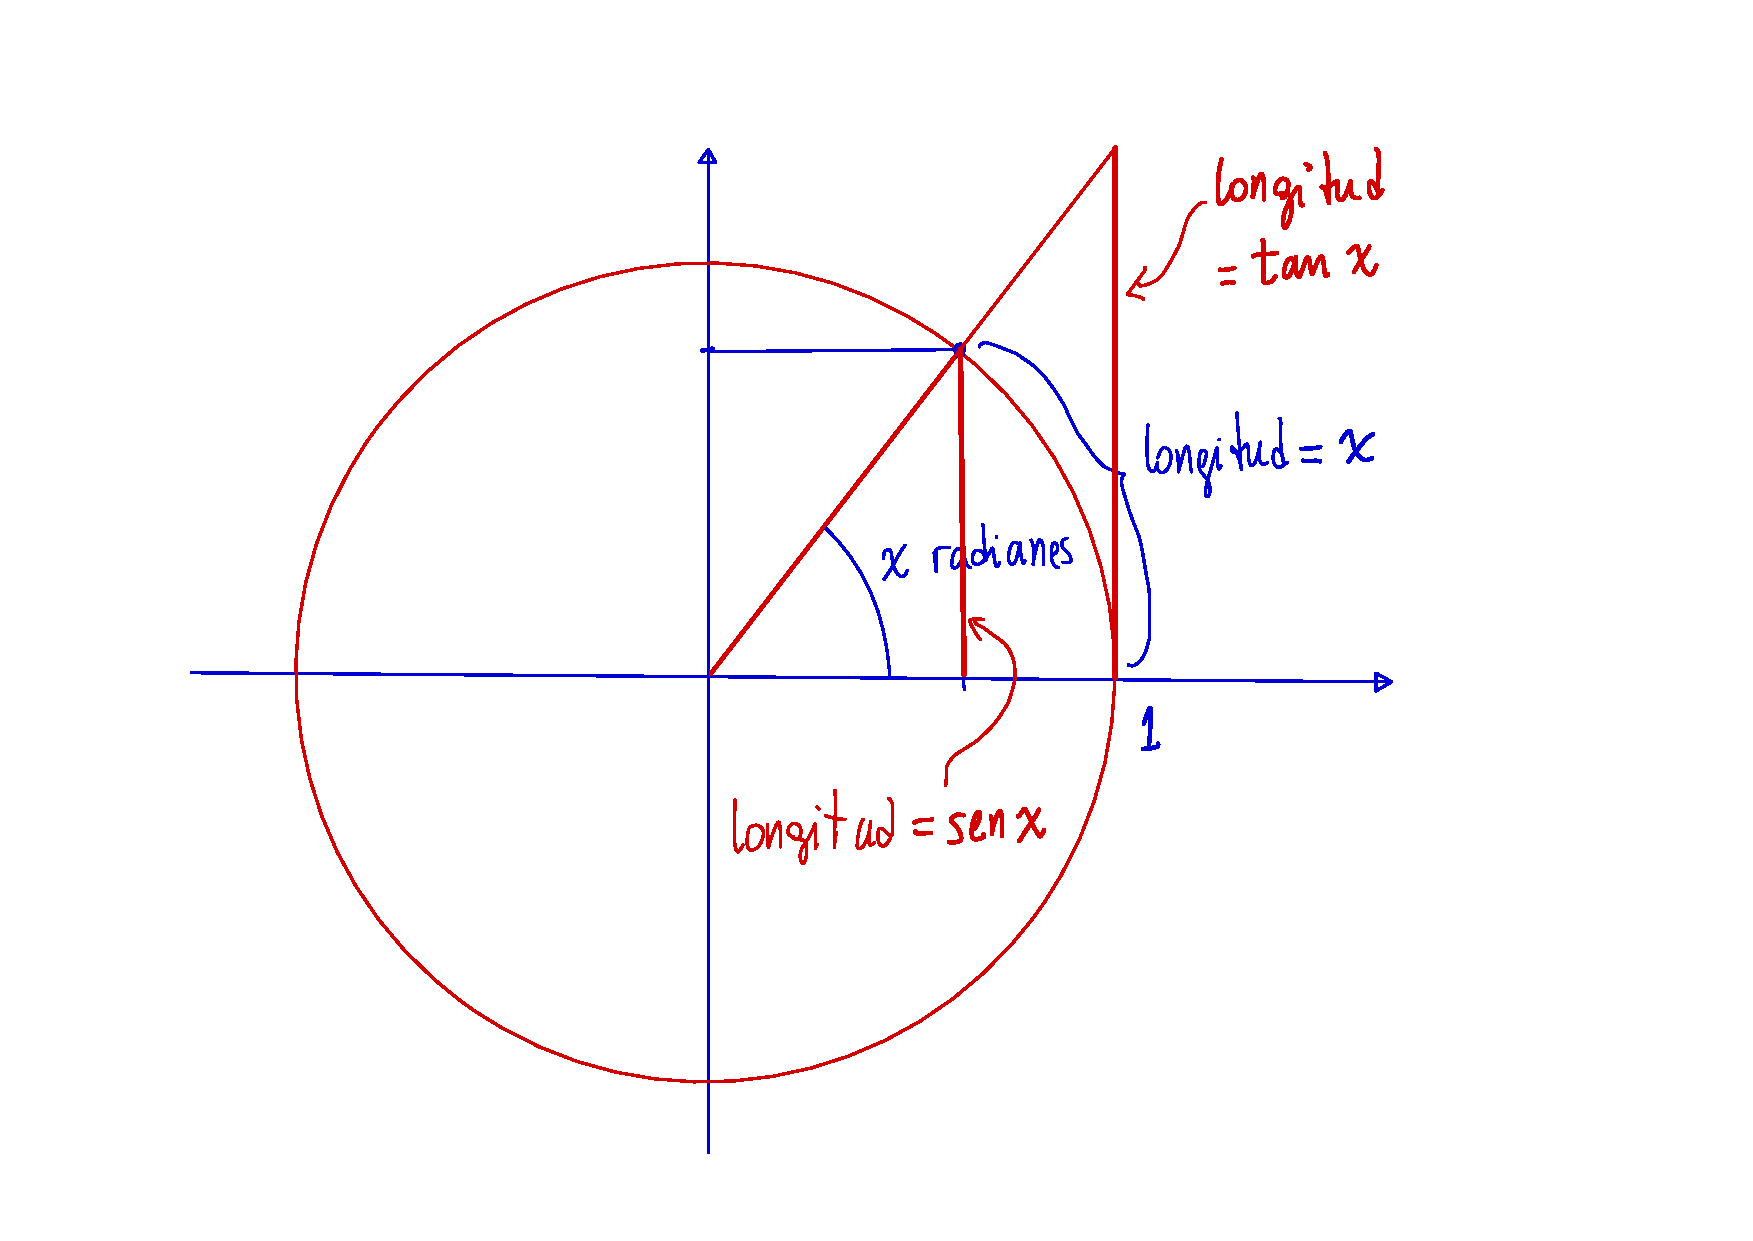
\includegraphics[width=.8\textwidth]{pics/seno-continuo.pdf}}

Utilizando ahora que la función seno es \emph{impar}, tenemos que para $-\pi/2<x<0$ resulta $\sen(x)=-\sen(-x)$ y por lo recién visto $0\le \sen(-x)\le -x$.
Por lo tanto,
\[
|\sen(x)|\le |x|, \qquad\text{para todo $x\in(-\pi/2,\pi,2)$}. 
\]
Esto implica que 
\[
-|x|\le \sen(x) \le |x|, \qquad\text{para todo $x\in(-\pi/2,\pi,2)$},
\]
y por la propiedad del emparedado, $\lim_{x\to0}\sen(x)=0=\sen(0)$, por lo que la función seno resulta continua en $x_0=0$.

Ahora bien, por identidades trigonométricas
\[
\sen(x)-\sen(x_0) = 2 \cos\frac{x+x_0}2 \sen\frac{x-x_0}2,
\]
y por lo tanto, como $|\cos(y)|\le 1$ cualquiera sea $y\in\R$,
\begin{align*}
|\sen(x)-\sen(x_0)| 
&= 2 \Big|\cos\frac{x+x_0}2\Big| \, \Big|\sen\frac{x-x_0}2\Big|
\\
&\le 2 \Big|\sen\frac{x-x_0}2\Big| 
\le 2 \Big|\frac{x-x_0}2\Big| ,
\end{align*}
si $|x-x_0|<\pi/2$. Esto muestra que $\D\limxo \big(\sen(x)-\sen(x_0)\big)=0$ o lo que es lo mismo 
\[
\limxo \sen(x)=\sen(x_0), \qquad \text{cualquiera sea $x_0\in\R$}.
\]
Por lo tanto, la función $f(x)=\sen(x)$ es continua en $\R$.
De manera similar, utilizando que
\[
\cos(x)-\cos(x_0) = -2 \sen\frac{x+x_0}2 \sen\frac{x-x_0}2,
\]
se puede probar que 
\[
\limxo \cos(x)=\cos(x_0), \qquad \text{cualquiera sea $x_0\in\R$},
\]
y por lo tanto, la función $f(x)=\cos(x)$ es continua en $\R$.

El resto de las funciones trigonométricas, como son cocientes de estas, resultan continuas en todo su dominio de definición, es decir, en todo $\R$, excepto en aquellos puntos donde el denominador se anula.

Como último ejemplo, estudiemos la continuidad de la función $f:\R\setminus\{0\}\to\R$ definida por
\[
f(x)=\frac{\sen(x)}{x}.
\]
Claramente esta función es continua en $\R\setminus\{0\}$ porque es el cociente de funciones continuas; notar que hemos quitado $x_0=0$ ya que allí el denominador de anula.

A priori no sabemos si existe $\D\lim_{x\to0}\frac{\sen(x)}{x}$ ya que tanto el numerador como el denominador tienden a cero.
Afirmamos que
\[
\lim_{x\to0}\frac{\sen(x)}{x}=1.
\]
Para ver que es así, notemos que para $0<x<\pi/2$, se cumple que 
\[
\sen(x)<x<\tan (x).
\]
Luego, dividiendo por $\sen(x)$ tenemos que
\[
1<\frac{\sen(x)}{x} < \frac{\tan(x)}{\sen(x)} = \frac{1}{\cos(x)}.
\]
Observamos ahora que como el coseno es continuo $\lim_{x\to 0^+}\cos(x)=\cos(0)=1$ y por el teorema del emparedado
\[
\lim_{x\to0^+}\frac{\sen(x)}{x}=1.
\]
Si $x<0$ resulta que $\D \frac{\sen(x)}{x} = \frac{\sen(-x)}{-x}$ y entonces
\[
\lim_{x\to0^-}\frac{\sen(x)}{x}
=\lim_{x\to0^-}\frac{\sen(-x)}{-x}
=\lim_{y\to0^+}\frac{\sen(y)}{y}=1.
\]
En definitiva, $\D f(x)=\frac{\sen(x)}{x}$ tiene una discontinuidad \emph{evitable} en $x_0=0$, que se evita definiendo $f(0)=1$.


\subsubsection*{Ejercicios de la sección~\getcurrentref{chapter}.\getcurrentref{section}}

\begin{enumerate}
\item Estudiar la continuidad en cada $x_0\in\R$ de las siguientes funciones:
\begin{multicols}{2}
\begin{enumerate}
    \item $\D f(x)=\frac{1}{x^2}$
    \item $\D f(x)=\begin{cases}
        \frac{x^2-3x+2}{x^2-4x+4}, \quad&\text{si }x > 3,\\
        2-x^2, \quad&\text{si }x \le 3
    \end{cases}$
    \item $\D f(x)=\begin{cases}
        \frac{x+3}{x-1}, \quad&\text{si }x\neq 1,\\
        2, \quad&\text{si }x = 1
    \end{cases}$
    \item $\D f(x)=\begin{cases}
        x^2+4, \quad&\text{si }x > 0,\\
        2x-1, \quad&\text{si }x <0
    \end{cases}$
    \item $\D f(x)=\frac{(x-3)^2}{x^2-9}$
    \item $\D f(x)=\frac{x^2}{\sqrt{1+x^2}-1}$
    \item $\D f(x)=\frac{\sqrt{1+x}-\sqrt{1-x}}{x}$
    \item $\D f(x)=\frac{4-\sqrt{6+x}}{2-\sqrt{x-2}}$
\end{enumerate}
\end{multicols}

\item Calcular los siguientes límites:
\begin{multicols}{2}
\begin{enumerate}
    \item $\D \lim_{x\to 2^+} \sqrt{\frac{x^3-9}{x^2-4}}$
    \item $\D \lim_{x\to 3} \sqrt{\frac{x^3-27}{x^2-9}}$
    \item $\D \lim_{x\to 0^+} \frac{\sqrt{1+x^2}-1}{x}$
    \item $\D \lim_{x\to 1} \frac{\sqrt{x+2}-\sqrt{3x+1}}{\sqrt{x-1}}$
    \item $\D \lim_{x\to 2^-} \sqrt{2-x}-\lfloor x+1 \rfloor$
    \item $\D \lim_{x\to 0} \frac{\sen 3x}{\sen 5x}$
    \item $\D \lim_{x\to 0} \frac{1-\cos x}x$
    \item $\D \lim_{x\to 0^+} \left(\sen x\right)^{\frac{\sen x}{x}}$
    \item $\D \lim_{x\to 0} \frac{\sen 3x}{x^2+\sqrt{x}}$
    \item $\D \lim_{x\to \pi/2} \frac{\cos x}{x-\pi/2}$
    \item $\D \lim_{x\to 0} \frac{\tan 2x}{3x}$
    \item $\D \lim_{x\to 0} \frac{x\, \sen x}{1-\cos x}$
    \item $\D \lim_{x\to 0} \frac{\ln(1+x)}{x}$
    \item $\D \lim_{x\to +\infty} \big(\ln(x+1)-\ln(x+2)\big)$
    \item $\D \lim_{x\to +\infty} \frac{\ln\big(1+e^x\big)}{x}$
    \item $\D \lim_{x\to -\infty} \frac{\ln\big(1+e^x\big)}{x}$
    \item $\D \lim_{x\to 0} \frac1x \, \ln\sqrt{\frac{1+x}{1-x}}$
    \item $\D \lim_{x\to 0} \left(1+x\right)^{\frac1{\sen x}}$
    \item $\D \lim_{x\to 0} \left(\cos x\right)^{1/x}$
    \item $\D \lim_{x\to +\infty} x^2 \big(\ln(x^2+4)-\ln x^2\big) $
\end{enumerate}
\end{multicols}


\end{enumerate}


    
\section{Funciones continuas en un intervalo cerrado}

Consideraremos en esta sección funciones $f$ que sean continuas en todos los puntos de un intervalo \emph{cerrado} $[a,b]$.
Hasta ahora solo hemos hablado de continuidad en intervalos abiertos; para definir continuidad en un punto $x_0$ hemos pedido que $x_0\in(a,b)$ con $(a,b)$ un intervalo abierto donde la función está definida.

\begin{definition}[Continuidad en un intervalo cerrado]
Decimos que una función $f:[a,b]\to\R$ es continua en $[a,b]$ si:
\begin{itemize}
    \item Es continua en $x_0$, para todo $x_0\in(a,b)$.
    \item Es continua \emph{por derecha} en $a$: $\D\lim_{x\to a^+}f(x)=f(a)$.
    \item Es continua \emph{por izquierda} en $b$: $\D\lim_{x\to b^-}f(x)=f(b)$.
\end{itemize}
\end{definition}

Las funciones continuas en intervalos cerrados tienen tres propiedades muy importantes. Para establecer la primera, necesitamos recordar que una función $f:A\to\R$ se dice \emph{acotada} si existen números reales $m$ y $M$ tales que 
\[
m\le f(x) \le M, \qquad\text{para todo $x\in A$}.
\]
En otras palabras, $f:A\to\R$ es acotada si la imagen de $f$, $\im(f)=\{f(x):x\in A\}$ es un conjunto acotado de $\R$.
Veamos el primer teorema importante.

\begin{theorem}\label{T:continua->acotada}
    Si $f:[a,b]\to\R$ es continua en $[a,b]$, entonces es acotada en $[a,b]$.
\end{theorem}

\begin{proof}
    La demostración de este teorema será vista en las clases de coloquios. El lector interesado puede encontrarla en el libro~\cite{Noriega}, como Teorema 6.25.
\end{proof}

Sigamos pensando en una función $f:[a,b]\to\R$ continua en el intervalo cerrado $[a,b]$. Ya vimos que es necesariamente acotada. Por lo tanto el conjunto $\im(f)$ es acotado, y entonces tiene supremo e ínfimo.
Lo que afirma el segundo resultado importante de esta sección es que ese supremo y ese ínfimo son, respectivamente, un máximo y un mínimo, es decir, existe $x_m\in[a,b]$ tal que $f(x_m)\le f(x)$, para todo $x\in[a,b]$, y existe $x_M\in[a,b]$ tal que $f(x_M)\ge f(x)$, para todo $x\in[a,b]$. Esto suele decirse de la siguiente forma: \emph{$f$ alcanza un máximo y un mínimo en $[a,b]$}.

\begin{theorem}\label{T:continua->maximo y minimo}
    Si $f$ es una función continua en un intervalo cerrado $[a,b]$, entonces alcanza un máximo y un mínimo en $[a,b]$.
\end{theorem}

\begin{proof}
    Al ser $f$ continua en $[a,b]$, el conjunto
    \[
    \im(f)=\{f(x) : x\in[a,b]\}
    \]
    es acotado inferior y superiormente, y claramente no vacío.
    Por lo tanto, existen
    \[
    m=\inf \im(f)
    \qquad\text{y}\qquad
    M=\sup \im(f).
    \]
    Probemos ahora que existe $x_M\in[a,b]$ tal que $f(x_1)=M$.
    Si no fuese cierto, entonces $f(x)<M$, para todo $x\in[a,b]$ y entonces $M-f(x)\neq 0$, para todo $x\in[a,b]$.
    Consideramos entonces la función
    \[
    g(x)=\frac{1}{M-f(x)},
    \]
    que resulta continua en $[a,b]$ porque es cociente de funciones continuas y el denominador no se anula en ese intervalo.
    Pero entonces, por el Teorema~\ref{T:continua->acotada} la función $g$ es acotada en $[a,b]$. En particular, existe $K>0$ tal que 
    \[
    g(x)=\frac{1}{M-f(x)}\le K,
    \qquad\text{para todo $x\in[a,b]$}.
    \]
    Esto a su vez implica que $\frac1K \le M -f(x)$ por lo que
    \[
    f(x)\le M-\frac1K,
    \qquad\text{para todo $x\in[a,b]$}.
    \]
    Es decir, $M-\frac1K$ es una cota superior de $\im(f)$.
    Como $M-\frac1K<M$ esto contradice que $M=\sup\im(f)$.
    Esta contradicción proviene de suponer que no existe $x_M\in[a,b]$ tal que $f(x_M)=M$.
    
    Luego, existe $x_M\in[a,b]$ tal que $f(x_M)=M$.
    Como $M$ es el supremo de la función $f$, resulta que es cota superior de $\im(f)$ y por lo tanto
    \[
    f(x_M)\ge f(x), 
    \qquad\text{para todo $x\in[a,b]$}.
    \]

    Razonando análogamente con la función
    \[
    h(x) = \frac1{f(x)-m}
    \]
    se prueba que existe $x_m\in [a,b]$ tal que $f(x_m)=m$, y por lo tanto
    \[
    f(x_m)\le f(x), 
    \qquad\text{para todo $x\in[a,b]$}.
    \qedhere
    \]
\end{proof}

Antes de ver el próximo teorema, conviene hacer algunas observaciones.

La idea original, intuitiva, geométrica, de una función continua, es la de una función cuya representación gráfica se puede hacer sin levantar el lápiz, es decir, que en la representación gráfica no haya saltos (como los que tiene la función $f(x)=\lfloor x\rfloor$) ni puntos donde la función se vaya al infinito (como $f(x)=\frac1x$ en $x=0$).

El siguiente teorema confirma nuestra intuición acerca de este significado geométrico de la continuidad.

\begin{theorem}[Teorema de Bolzano]\label{T:Bolzano}
Sea $f$ una función continua en $[a,b]$ tal que $f(a)<0$ y $f(b)>0$. Entonces existe $c\in(a,b)$ tal que $f(c)=0$.
\end{theorem}

Este teorema afirma que si un punto de la gráfica de una función continua está por debajo del eje de abscisas y otro está por encima, entonces dicha gráfica debe cortar el eje de abscisas en algún punto.

\begin{proof}
    Consideremos el conjunto
    \[
    A=\{x\in[a,b]:f(x)<0\}.
    \]
    Este conjunto está acotado superiormente por $b$ y es no vacío ya que $a\in A$.
    Entonces existe $c=\sup A$. Afirmamos que ese $c$ cumple $f(c)=0$. Para probarlo, descartaremos las posibilidades $f(c)<0$ y $f(c)>0$.

    Si fuera $f(c)<0$, entonces, por la Proposición~\ref{P:continua:cota en intervalo}, existe $\delta>0$ tal que $f(x)<0$ para todo $x\in(c-\delta,c+\delta)$. Tomamos $x_1=c+\delta/2$ que cumple $c<x_1<c+\delta$ y entonces $f(x_1)<0$. Luego $x_1>c$ y $x_1\in A$, lo que contradice que $c=\sup A$ (contradice que $c$ sea cota superior de $A$). Por lo tanto, no es posible que $f(c)<0$.

    Supongamos ahora que $f(c)>0$, nuevamente por la Proposición~\ref{P:continua:cota en intervalo}, existe $\delta>0$ tal que $f(x)>0$ para todo $x\in (c-\delta,c+\delta)$. Tomamos $x_2=c-\delta/2$ que cumple $c-\delta<x_2<c$ y entonces $x_2<c$ y no podría ser cota superior de $A$ (ya que al ser $c=\sup A$ es la menor de las cotas superiores).
    Como $x_2<c$ no es cota superior, debe existir $x_3\in A$ tal que $x_2<x_3\le c$. Pero $x_3\in(c-\delta,c+\delta)$ por lo que $f(x_3)>0$, lo que contradice que $x_3\in A$.
    Por lo tanto, no es posible que $f(c)>0$.
\end{proof}

A partir de este teorema, concluimos el famoso \emph{Teorema del Valor Intermedio (TVI)}.

\begin{corollary}[Teorema del Valor Intermedio]\label{TVI}
Sea $f$ una función continua en $[a,b]$ tal que $f(a)<f(b)$.
Si $d$ es cualquier número tal que $f(a)<d<f(b)$, entonces existe $c\in(a,b)$ tal que $f(c)=d$.
\end{corollary}

\begin{proof}
    Definimos la función auxiliar
    \[
    g(x) = f(x)-d.
    \]
    Esta función es también continua en $[a,b]$ y cumple 
    \[
    g(a) = f(a)-d < 0,
    \qquad\text{y}\qquad
    g(b) = f(b)-d > 0.
    \]
    Luego, por el Teorema~\ref{T:Bolzano}, existe $c\in(a,b)$ tal que $g(c)=0$.
    Como $g(c)=f(c)-d$, $g(c)=0$ equivale a $f(c)=d$.
\end{proof}

Como consecuencia de este último resultado, se obtiene la continuidad de algunas funciones.

\begin{theorem}[Continuidad de la función inversa]
Si $f$ es una función continua en $[a,b]$ y estrictamente creciente (o estrictamente decreciente) en $[a,b]$, entonces
\begin{enumerate}[{\bf (a)}]
    \item $f:[a,b]\to[f(a),f(b)]$ ($f:[a,b]\to[f(b),f(a)]$) es biyectiva.
    \item $f^{-1}:[f(a),f(b)]\to [a,b]$ ($f^{-1}:[f(b),f(a)]\to [a,b]$) es continua.
\end{enumerate}
\end{theorem}

\begin{proof}
    Demostremos el caso en que $f$ es estrictamente creciente (el caso de $f$ estrictamente decreciente es análogo).

\begin{enumerate}[{\bf (a)}]
\item $f$ es inyectiva, dado que es \emph{estrictamente} creciente. $f$ es sobreyectiva, pues si $y\in (f(a),f(b))$ resulta $f(a)<y<f(b)$ y por lo tanto, por el Teorema~\ref{TVI} existe $x\in(a,b)$ tal que $f(x)=y$.

\item Ya que $f$ es biyectiva, tiene función inversa $f^{-1}:[f(a),f(b)]\to [a,b]$. Veamos que $f^{-1}$ es continua en cada $y_0\in(f(a),f(b))$. 

Sea $y_0\in(f(a),f(b))$ y sea $\epsilon>0$; suponemos que $\epsilon<\min\{b-x_0,x_0-a\}$ ya que lo importante es lo que ocurre para $\epsilon$ pequeño. Al ser $f$ sobreyectiva, existe $x_0\in(a,b)$ tal que $f(x_0)=y_0$.
Sean
\[
d_1=f(x_0-\epsilon), 
\qquad
d_2=f(x_0+\epsilon),
\]
y sea
\[
\delta=\min\{d_2-y_0,y_0-d_1\}
\qquad\text{luego $\delta\le d_2-y_0$ y $\delta\le y_0-d_1$}.
\]
Queremos probar que $|y-d|<\delta$ implica $\big|f^{-1}(y)-f^{-1}(y_0)\big|<\epsilon$.
Para ello, sea $y$ tal que $|y-d|<\delta$, o sea $y_0-\delta<y<y_0+\delta$.
Como $f$ es sobreyectiva, existe $c\in(a,b)$ tal que $f(c)=y$.
Siendo $y_0-\delta<y<y_0+\delta$, resulta $d_1<y<d_2$, o sea
\[
d_1=f(x_0-\epsilon)<y=f(c)<f(x_0+\epsilon)=d_2.
\]
Como $f$ es estrictamente creciente, debe ser
\[
x_0-\epsilon < c < x_0+\epsilon 
\quad\implies\quad
|c-x_0|<\epsilon.
\]
Pero $c=f^{-1}(y)$ y $x_0=f^{-1}(y_0)$ por lo que
\[
\big|f^{-1}(y)-f^{-1}(y_0)\big|<\epsilon.
\]
Hemos demostrado que dado $\epsilon>0$ existe $\delta$ tal que
\[
\big|f^{-1}(y)-f^{-1}(y_0)\big|<\epsilon,
\qquad\text{para todo $y$ tal que $|y-y_0|<\delta$}.
\]
Es decir, $f\inv$ es continua en $y_0$, cualquiera sea $y_0\in(f(a),f(b))$.
La demostración de que $f\inv$ es continua por derecha en $y_a=f(a)$ y que es continua por izquierda en $y_b=f(b)$ es análoga.
\end{enumerate}
\end{proof}


\subsubsection*{Ejercicios de la sección~\getcurrentref{chapter}.\getcurrentref{section}}

\begin{enumerate}
\item Para las siguientes funciones, determinar cuáles son acotadas superiormente e inferiormente en el intervalo indicado y si alcanzan su máximo y mínimo en algún punto del intervalo:

\begin{multicols}{2}
\begin{enumerate}
    \item $f(x)= x^2$ en $(-1,1)$
    \item $f(x)= x^2$ en $[-1,1]$
    \item $f(x)= x^3$ en $(-1,1)$
    \item $f(x)= x^3$ en $[-1,1]$
    \item $\D f(x)= \frac1x$ en $(0,1)$
    \item $\D f(x)= \frac1x$ en $(0,1]$
    \item $f(x)= \sqrt{x}$ en $(0,1)$
    \item $f(x)= \sqrt{x}$ en $[0,1]$
\end{enumerate}   
\end{multicols}



\item Probar que la ecuación $x^3-3x+1=0$ tiene una raíz real en el intervalo $(1,2)$.

\item Probar que existe $x\in\R$ tal que $\cos x=x$.

\item Probar que si $p(x)$ es un polinomio \emph{mónico} de grado impar, entonces existe $x_0\in\R$ tal que $p(x_0)=0$.

\item Probar que si $p(x)$ es un polinomio de grado impar, entonces existe $x_0\in\R$ tal que $p(x_0)=0$.

\item Probar que si $n$ es un número natural, entonces en el intervalo $\D\Big(n\pi-\frac\pi2,n\pi+\frac\pi2\Big)$ hay un $x$ que cumple $\tan x=-x$. Ayudarse con GeoGebra, graficar las funciones $\tan x$ y $-x$ para ver cómo usar el Teorema~\ref{TVI} para demostrar lo pedido.

\item Demostrar que existe un número real $x$ tal que
\[
x^{179} + \frac{163}{1+x^2+\sen^2 x} = 119.
\]

\item Supongamos que $f$ y $g$ son continuas en $\R$ y que $f(a)>g(a)$ para algún $a\in\R$ y $f(b)<g(b)$ para algún $b\in\R$. Probar que existe $x\in\R$ tal que $f(x)=g(x)$.

\item Supongamos que $f:\R\to\R$ es continua y que $f(x)\in\Q$, para todo $x\in\R$. Probar que entonces $f$ es constante.

\end{enumerate}

\section{El método de Bisección}

Como consecuencia del Teorema del Valor Intermedio se obtiene un método para calcular de manera aproximada soluciones de ecuaciones para las cuales no hay un fórmula precisa.
Por ejemplo, las ecuaciones
\[
\cos x = x,\qquad
\ln x = \frac 1x,\qquad
x = e^x-2, \qquad
x\sen(x)=1.
\]

Todas estas ecuaciones pueden escribirse como
\begin{equation}\label{eq:ecuacion1}
f(x) = 0.
\end{equation}
En efecto, si restamos el lado derecho del izquierdo en cada ecuación de los ejemplos presentados, tenemos
\[
\cos x - x=0,\qquad
\ln x - \frac 1x=0,\qquad
x - e^x + 2=0, \qquad
x\sen(x)-1=0.
\]

Un corolario inmediato del Teorema del Valor Intermedio~\ref{TVI} es el siguiente:

\begin{corollary}
Si $f:[a,b] \to \R$ es una función continua y $f(a)$ y $f(b)$ tienen signo opuesto ($f(a)\cdot f(b) < 0$), entonces existe $c \in (a,b)$ tal que $f(c) = 0$.
\end{corollary}

La idea del método de bisección es comenzar con un intervalo $[a,b]$ tal que $f(a)$ y $f(b)$ tienen signo opuesto, es decir, tenemos localizada una raíz en el intervalo $[a,b]$. Luego, ir reduciendo sistemáticamente la longitud del intervalo donde estamos seguros que hay una raíz, hasta que tengamos una tolerancia aceptable, es decir, un intervalo tan pequeño donde se encuentra la raíz que es satisfactorio para el problema en cuestión.
La manera de subdividir el intervalo consiste en tomar el punto medio del intervalo 
\[
m = \frac{a+b}2,
\]
y luego analizar las tres posibilidades que pueden darse
\begin{enumerate}[(1)]
\item Si $f(a)$ y $f(m)$ tienen signos opuestos, entonces hay un cero en $[a,m]$.
\item Si $f(m)$ y $f(b)$ tienen signos opuestos, entonces hay un cero en $[m,b]$.
\item Si $f(m) = 0$, entonces $m$ es la solución buscada.
\end{enumerate}

Si ocurre el caso (3), hemos encontrado la raíz (debemos aclarar que esto no se da casi nunca, pero puede ocurrir).
Si ocurre el caso (1) o el caso (2), entonces hemos encontrado un intervalo cuyo ancho es la mitad que el original y contiene una raíz. Para continuar el proceso, renombramos el nuevo intervalo más pequeño como $[a,b]$ y repetimos el procedimiento hasta que el intervalo sea tan pequeño como deseamos. Puesto que el proceso de bisección genera una sucesión de intervalos encajados, con sus correspondientes puntos medios, usaremos la siguiente notación para tener un registro de los detalles del proceso:\\

\frame{
\begin{minipage}{.9\textwidth}
${}$	

\centerline{\bf Método de Bisección}
\begin{itemize}
\item $[a_0,b_0]$ es el intervalo de partida y $m_0 = \D\frac{a_0+b_0}2$ es su punto medio.
\item $[a_1,b_1]$ es el segundo intervalo (coincide con $[a_0,m_0]$ o con $[m_0,b_0]$) y $m_1$ es su punto medio. El intervalo $[a_1,b_1]$ es la mitad de ancho que $[a_0,b_0]$.
\item $\cdots$
\item Después de llegar al intervalo $[a_n,b_n]$, en el que también se localiza un cero, y cuyo punto medio es $m_n$, se construye el intervalo $[a_{n+1},b_{n+1}]$, en el que también hay un cero y mide la mitad de $[a_n,b_n]$.\\
\end{itemize}
\end{minipage}
}

A partir de este procedimiento resulta que
\[
a_0 \le a_1 \le \dots \le a_n \le \dots \le b_n \le \dots\le b_1 \le b_0.
\]
Y además, hay una raíz $c$ que satisface $a_n \le c \le b_n$.

Es importante que nos detengamos un momento a pensar cómo se define el intervalo $[a_{n+1},b_{n+1}]$ a partir del $[a_n,b_n]$:
\begin{itemize}
\item Definimos $m_n = \D\frac{a_n+b_n}2$.
\item Si $f(a_n)\cdot f(m_n) < 0$ (entonces hay una raíz en el intervalo $[a_n,m_n] $)
\begin{itemize}
\item Definimos $[a_{n+1},b_{n+1}] = [a_n,m_n]$ (o $a_{n+1} = a_n$ y $b_{n+1} = m_n$)
\end{itemize}
\item Si no, (entonces ocurre que $f(m_n)\cdot f(b_n) < 0$)
\begin{itemize}
\item Definimos $[a_{n+1},b_{n+1}] = [m_n,b_n]$ (o $a_{n+1} = m_n$ y $b_{n+1} = b_n$)
\end{itemize}
\item Si no ocurre ninguna de las anteriores, resulta $f(m_n)=0$. 
\begin{itemize}
\item Entonces $m_n$ es la solución. FIN.
\end{itemize}
\end{itemize}

Observamos que con este procedimiento, en cada paso, la longitud del intervalo se reduce a la mitad, es decir
\[
|b_{n+1} - a_{n+1}| = \frac{|b_n-a_n|}2.
\]

Por lo tanto, después de $n$ pasos, la longitud del intervalo es
\[
|b_n - a_n| = \frac{|b_0-a_0|}{2^n} = \left(\frac12\right)^n |b_0-a_0|.
\]

Como $m_n$ está en el centro del intervalo $[a_n,b_n]$ resulta que la distancia a la raíz $c$ es menor o igual a la mitad de la longitud del intervalo $[a_n,b_n]$, es decir
\[
|c - m_n| \le \frac{|b_n-a_n|}2 = \left(\frac12\right)^{n+1} |b_0-a_0|.
\]

Resumimos todo lo analizado hasta ahora en el siguiente teorema.

\begin{theorem}[Convergencia del método de bisección]
Supongamos que $f:[a,b] \to \R$ es continua y que $f(a)$ y $f(b)$ tienen signos distintos.
Sea $\{ m_n \}_{n\ge 0}$ la sucesión de puntos medios de los intervalos generados por el método de bisección. Entonces existe una raíz $c$ de la ecuación $f(x)=  0$ (es decir, $f(c)=0$) en $[a,b]$ tal que $m_n \to c$, cuando $n\to\infty$ y además
\[
|c - m_n | \le \left(\frac12\right)^{n+1} |b-a|, \qquad n=0,1,2,\dots.
\]
\end{theorem}

\subsubsection*{Ejercicios de la sección~\getcurrentref{chapter}.\getcurrentref{section}}

\begin{enumerate}
\item Programar en \verb|Python| el método de bisección.

\item Utilizar el método programado en el punto anterior para hallar una solución aproximada de cada una de las siguientes ecuaciones en el intervalo indicado. Se pide una solución con un error menor a $10^{-6}$.
\begin{multicols}{2}
    \begin{enumerate}
        \item $\D \cos x = x$ en $[0,\pi/2]$
        \item $\D \ln x = 1/x$ en $[1,3]$
        \item $\D x=e^x-2$ en $[0,2]$
        \item $\D x\sen(x)=1$ en $[0,2]$
    \end{enumerate}
\end{multicols}

\end{enumerate}

\begin{comment}

\section{Continuidad uniforme (LMA???)}


\subsubsection*{Ejercicios de la sección~\getcurrentref{chapter}.\getcurrentref{section}}

\begin{enumerate}
\item 
\end{enumerate}




\end{comment}


%%%%%%%%%%%%%%%%%%%%%% ejercicios del capítulo
\subsection*{Ejercicios del capítulo~\getcurrentref{chapter}}


\begin{enumerate}
\item Demostrar que la función $f(x)=-3x+10$ es continua en $x_0$, para todo $x_0\in\R$.

\item 
Consideremos la función $f:(0,\infty)\to(0,\infty)$ dada por
$f(x)=\frac1x$.
\begin{enumerate}
    \item Demostrar que es continua en $x_0=2$;
    \item Demostrar que es continua en $x_0=1$;
    \item Demostrar que es continua en $x_0=1/2$;
    \item ¿Se anima a demostrar que es continua en $x_0$, cualquiera sea  $x_0>0$?
\end{enumerate}

\item 
Consideremos la función $f:(0,\infty)\to(0,\infty)$ dada por
$f(x)=\sqrt x$.
\begin{enumerate}
    \item Demostrar que es continua en $x_0=2$;
    \item Demostrar que es continua en $x_0=1$;
    \item Demostrar que es continua en $x_0=1/2$;
    % \item Demostrar que es continua en $x_0=0$;
    \item ¿Se anima a demostrar que es continua en $x_0$, cualquiera sea $x_0\in(0,\infty)$?
\end{enumerate}

\item 
Consideremos la función 
\[
f(x) = \begin{cases}
    x\sen \frac1x,\quad &\text{si $x\neq 0$},
    \\
    0,\quad &\text{si $x = 0$},
    \end{cases}
\]
\begin{enumerate}
    \item Graficarla con GeoGebra
    \item Verificar con geogebra que 
    \[
    -|x| \le f(x) \le |x|,\quad \forall\xiR.
    \]
    \item Demostrar analíticamente que 
    \[
    -|x| \le f(x) \le |x|,\quad \forall\xiR.
    \]
    \item Verificar que $|f(x)-f(0)|\le |x-0|$, para todo \xiR.
    \item Demostrar que $f(x)$ es continua en $x_0=0$.
\end{enumerate}

\item 
Consideremos la función
\[
H(x) = \begin{cases}
    0, \quad &\text{si $x<0$},\\
    1, \quad &\text{si $x\ge0$},
\end{cases}
\]
\begin{enumerate}
    \item Demostrar que $H(x)$ es continua en $x_0$ para todo $x_0\neq 0$.
    \item Demostrar que $H(x)$ no es continua en $x_0=0$.
\end{enumerate}

\item \label{ej:sen1_x}
Consideremos la función 
\[
f(x) = \begin{cases}
    \sen \frac1x,\quad &\text{si $x\neq 0$},
    \\
    0,\quad &\text{si $x = 0$},
    \end{cases}
\]
\begin{enumerate}
    \item Graficarla con GeoGebra
    \item Demostrar que para cada $\delta>0$ existe $x_1\in(0,\delta)$ tal que $f(x_1)=1$.
    \item Demostrar que para cada $\delta>0$ existe $x_2\in(0,\delta)$ tal que $f(x_2)=-1$.
    \item Demostrar que $f(x)$ no es continua en $x_0=0$.
\end{enumerate}


\item Consideremos la función constante $f(x)=a$, para algún $a\in\R$. Demostrar usando la definición que $f$ es continua en $x_0$ para todo $x_0\in\R$.
\item Consideremos la función \emph{identidad} $f(x)=x$. Demostrar usando la definición que $f$ es continua en $x_0$ para todo $x_0\in\R$.
\item Demostrar que si $a$ y $b$ son números reales, entonces la función lineal $f(x)=ax+b$ es continua en $x_0$ para todo $x_0\in\R$.
Usar lo demostrado en los ejercicios anteriores y las propiedades vistas en esta sección.
\item Demostrar que si $a$, $b$ y $c$ son números reales, entonces la función cuadrática $f(x)=ax^2+bx+c$ es continua en $x_0$ para todo $x_0\in\R$.
Usar lo demostrado en los ejercicios anteriores y las propiedades vistas en esta sección.
\item\label{ej:polinomios-continuos} Demostrar que si $p(x)$ es una función polinomial, entonces $p$ es continua en $x_0$ para todo $x_0\in\R$ (Ayuda: usar inducción sobre el grado polinomial).
\item Demostrar que si $p(x)$ y $q(x)$ son funciones polinomiales, entonces la función racional $\frac pq$ es continua en $x_0$ para todo $x_0\in\R$, excepto para aquellos puntos donde $q(x)$ se anula. 


\item Demostrar usando la definición, que $\D\lim_{x\to 0^+} \sqrt{x} = 0$.

\item Demostrar usando el Teorema~\ref{T:TFLD} que no existe $\D\lim_{x\to 0^+}\cos\frac1x$.

\item Determinar (usando los límites que ya conocemos y las propiedades) los siguientes límites, considerando separadamente los casos $x_0\in\Z$ y $x_0\in\R\setminus\Z$:
\begin{multicols}{2}
    \begin{enumerate}
    \item $\D\lim_{x\to x_0^+} \big(x-\lfloor x \rfloor\big)$;
    \item $\D\lim_{x\to x_0^+} \big(|x|+\lfloor x \rfloor\big)$.
    \end{enumerate}
\end{multicols}

\item Determinar (usando los límites que ya conocemos y las propiedades) los siguientes límites, considerando separadamente los casos $x_0=0$ y $x_0\neq 0$:
\begin{multicols}{2}
    \begin{enumerate}
    \item $\D\lim_{x\to x_0^+} \big(x+\sgn(x))$;
    \item $\D\lim_{x\to x_0^+} \big(x\cdot \sgn(x)\big)$.
    \end{enumerate}
    \end{multicols}

\item Demostrar que $\D\lim_{x\to 0^+} x \sen\frac1x = 0$ (?`qué teorema conviene usar para esto?).
    

\item Demostrar que no existe $\D\lim_{x\to 0^-}\sen\frac1x$.

\item Demostrar que no existe $\D\lim_{x\to 0^-}\cos\frac1x$.

\item Determinar los siguientes límites, considerando separadamente los casos $x_0\in\Z$ y $x_0\in\R\setminus\Z$:
\begin{multicols}{2}
    \begin{enumerate}
    \item $\D\lim_{x\to x_0^-} \big(x-\lfloor x \rfloor\big)$;
    \item $\D\lim_{x\to x_0^-} \big(|x|+\lfloor x \rfloor\big)$.
    \end{enumerate}
\end{multicols}

\item Determinar los siguientes límites, considerando separadamente los casos $x_0=0$ y $x_0\neq 0$:
\begin{multicols}{2}
    \begin{enumerate}
    \item $\D\lim_{x\to x_0^-} \big(x+\sgn(x))$;
    \item $\D\lim_{x\to x_0^-} \big(x\cdot \sgn(x)\big)$.
    \end{enumerate}
    \end{multicols}

\item Demostrar que $\D\lim_{x\to 0^-} x \sen\frac1x = 0$.

\item Probar usando la definición que se cumplen las siguientes afirmaciones:

\begin{multicols}{2}
    \begin{enumerate}
        \item $\D \lim_{x\to 2} 3x-1=5 $.
        \item $\D \lim_{x\to 3} 4 x^2 = 36$.
        \item $\D \lim_{x\to 2} 3/x = 3/2$.
        \item $\D \lim_{x\to 1} x^2+2x = 3$.
    \end{enumerate}
\end{multicols}

\item Analizar la existencia de los siguientes límites:
\begin{multicols}{2}
    \begin{enumerate}
\item $\D \lim_{x\to 0} \sen \frac1x$;
\item $\D \lim_{x\to 0} \cos \frac1x$;
\item $\D \lim_{x\to 0} \sgn(x)$;
\item $\D \lim_{x\to 0} x \sen \frac1x$;
\item $\D \lim_{x\to 0} x^2 \sen \frac1x$;
\item $\D \lim_{x\to 0} (x + \sen \frac1x)$.
\end{enumerate}
\end{multicols}

\item ?`Para qué valores de $x_0\in\R$ existe $\limxo \lfloor x \rfloor$?

\item ?`Para qué valores de $x_0\in\R$ existe $\limxo \big(x - \lfloor x \rfloor\big)$?

\item Analizar la veracidad o falsedad de las siguientes afirmaciones:
\begin{enumerate}
    \item Si existe $\D\limxo \big(f(x)+g(x)\big)$, entonces existen
    $\D\limxo f(x)$ y $\D\limxo g(x)$.
    \item Si existe $\D\limxo \big(f(x)+g(x)\big)$ y existe
    $\D\limxo f(x)$, entonces existe $\D\limxo g(x)$.
    \item Si existe $\D\limxo \big(f(x)\cdot g(x)\big)$, entonces existen
    $\D\limxo f(x)$ y $\D\limxo g(x)$.
    \item Si existe $\D\limxo \big(f(x)\cdot g(x)\big)$ y existe
    $\D\limxo f(x)$, entonces existe $\D\limxo g(x)$.
    \item Si existe $\D\limxo \big(f(x)\cdot g(x)\big)$ y existe
    $\D\limxo f(x)\neq 0$, entonces existe $\D\limxo g(x)$.
    
\end{enumerate}

\item Sea $a>0$, $a\neq 1$ y supongamos que $\limxo f(x)=\ell>0$.
Demostrar que $\D\limxo \log_a(f(x)) = \log_a(\ell).$ (Recordar que $\D\log_a y = \frac{\ln y}{\ln a}$).

\item Consideremos la función constante $f(x)=a$, para algún $a\in\R$. Demostrar usando la definición que $\limxo f(x)=f(x_0)$, cualquiera sea $x_0\in\R$.
\item Consideremos la función \emph{identidad} $f(x)=x$. Demostrar usando la definición que $\limxo f(x)=f(x_0)$, cualquiera sea $x_0\in\R$.
\item Demostrar que si $a$ y $b$ son números reales, entonces la función lineal $f(x)=ax+b$ cumple que $\limxo f(x)=f(x_0)$, cualquiera sea $x_0\in\R$.
Usar lo demostrado en los ejercicios anteriores y las propiedades vistas en esta sección.
\item Demostrar que si $a$, $b$ y $c$ son números reales, entonces la función cuadrática $f(x)=ax^2+bx+c$ cumple que $\limxo f(x)=f(x_0)$, cualquiera sea $x_0\in\R$.
Usar lo demostrado en los ejercicios anteriores y las propiedades vistas en esta sección.
\item Demostrar que si $p(x)$ es una función polinomial, entonces $\limxo p(x)=p(x_0)$, cualquiera sea $x_0\in\R$.
\item Demostrar que si $p(x)$ y $q(x)$ son funciones polinomiales, entonces para la función racional $f(x)= \frac{p(x)}{q(x)}$ se cumple que $\limxo f(x)=f(x_0)$, cualquiera sea $x_0\in\R$, si $q(x_0)\neq0$.


\item Calcular los siguientes límites.
 Si el límite es infinito, indicar si es $+\infty$, $-\infty$ o meramente $\infty$.
   
\begin{multicols}{2}
    \begin{enumerate}
        \item $\D\lim_{x\to0} \frac{1}{x+x^2}$
        \item $\D\lim_{x\to0} \frac{1}{x^2+x^4}$
        \item $\D\lim_{x\to0} \frac{-1}{|x|}$
        \item $\D\lim_{x\to0^+} \frac{1}{\sqrt x}$
        \item $\D\lim_{x\to2} \frac{3}{(x-2)^2}$
        \item $\D\lim_{x\to0} \frac{x}{\sqrt{x^2+1}-1}$
    \end{enumerate}
\end{multicols}

\item Escribir proposiciones que relacionen todas las definiciones de límites de la Sección~\getcurrentref{chapter}.\getcurrentref{section} con límites de sucesiones.

\item Analizar la existencia de los siguientes límites:
   
\begin{multicols}{2}
    \begin{enumerate}
        \item $\D\lim_{x\to+\infty} \sen(x)$
        \item $\D\lim_{x\to+\infty} \cos(x)$
        \item $\D\lim_{x\to+\infty} \frac{\sen(x)}x$
        \item $\D\lim_{x\to+\infty} x\sen\Big(\frac\pi x\Big)$
        \item $\D\lim_{x\to0} \frac{|x|-x}{|x|+x}$
        \item $\D\lim_{x\to0} x\cdot\lfloor x \rfloor$
        \item $\D\lim_{x\to0} x\cdot\bigg\lfloor \frac1x \bigg\rfloor$
    \end{enumerate}
\end{multicols}

\item Calcular los siguientes límites.
 Si el límite es infinito, indicar si es $+\infty$, $-\infty$ o meramente $\infty$.
   
\begin{multicols}{2}
    \begin{enumerate}
    \item $\D \lim_{x\to+\infty} \frac{x^3+2x-1}{2x^3-3x+4}$
    \item $\D \lim_{x\to-\infty} \frac{x^3+2x-1}{2x^3-3x+4}$
    \item $\D \lim_{x\to+\infty} \frac{2x^2-3x}{x^3+1}$
    \item $\D \lim_{x\to-\infty} \frac{2x^2-3x}{x^3+1}$
    \item $\D \lim_{x\to+\infty} \frac{\sqrt{x^2+x+1}+\sqrt{x^2-x+1}}{x+\sqrt{x^2+1}}$
    \item $\D \lim_{x\to-\infty} \frac{\sqrt{x^2+x+1}+\sqrt{x^2-x+1}}{x+\sqrt{x^2+1}}$
    \item $\D \lim_{x\to+\infty} \frac{2+x^{5/3}}{3x+x^{1/5}}$
    \item $\D \lim_{x\to-\infty} \frac{2+x^{5/3}}{3x+x^{1/5}}$
    \item $\D \lim_{x\to+\infty} \frac{\sqrt{x}+x^{3/4}}{x^{1/3}+x^{2/3}}$
    \item $\D \lim_{x\to-\infty} \frac{x^2-1}{x+2}-\frac{x^2+1}{x+2}$
    \item $\D \lim_{x\to+\infty} \frac{\sqrt{x+1}-\sqrt{x-1}}{\sqrt{x+1}+\sqrt{x-1}}$
    \item $\D \lim_{x\to+\infty} x^2-2x$
    \item $\D \lim_{x\to+\infty} 2x^2+6x$
    \item $\D \lim_{x\to+\infty} \frac{\sqrt{x+\sqrt{x}}}{\sqrt{x+\sqrt{x+\sqrt{x}}}}$
    \item $\D \lim_{x\to+\infty} x\big(x-\sqrt{2x^2+3}\big)$
    \item $\D \lim_{x\to+\infty} \sqrt{x^2+2x}-x$
    \item $\D \lim_{x\to+\infty} x+\sqrt{1-x^3}$
    \item $\D \lim_{x\to+\infty} \bigg(\frac{x+1}{x+2}\bigg)^{2x}$
    \item $\D \lim_{x\to+\infty} \bigg(\frac{2x^2+5}{x^2+1}\bigg)^{3x^2+1}$
    \item $\D \lim_{x\to+\infty} \bigg(\frac{x+4}{x+6}\bigg)^{x^2}$
    \item $\D \lim_{x\to+\infty} \bigg(\frac{x^2+1}{x^2+2}\bigg)^{x^3}$
    
    
    \end{enumerate}
\end{multicols}


\item Determinar cuáles de las siguientes funciones cumplen que $f(h)=o(h)$:
\begin{multicols}{2}
\begin{enumerate}
    % \item $f(x) = x^2$
    \item $f(x) = x^3$
    \item $f(x) = 1$
    \item $f(x) = |x|^{1.001}$
    \item $f(x) = |x|^\alpha$ con $\alpha > 1$
    \item $f(x) = |x|^{1/3}$
    \item $f(x) = |x|$
    \item $f(x) = |x|^\alpha$ con $\alpha \le 1$
    \item $f(x) = \frac{x}{\log |x|}$
    % \item $f(x) = 1-\cos(x)$
    \item $f(x) = \log(|x|)$
    \item $f(x) = e^x$
    \item $f(x) = e^{-1/|x|}$
    
    % \item $f(x) = \sen(x)$, 
\end{enumerate}    
\end{multicols}

\item Demostrar las siguientes afirmaciones:
    \begin{enumerate}
        \item Si $f(h)=o(h)$, entonces $cf(h) = o(h)$.
        \item Si $f(h)=o(h)$ y $g(h) = o(h)$, entonces $f(h)+g(h) = o(h)$.
        \item Si $f(h)=o(h)$ y $g(h) = o(h)$, entonces $f(h)g(h) = o(h)$.
    \end{enumerate}

\item Estudiar la continuidad en cada $x_0\in\R$ de las siguientes funciones:
\begin{multicols}{2}
\begin{enumerate}
    \item $\D f(x)=\frac{1}{x^2}$
    \item $\D f(x)=\begin{cases}
        \frac{x^2-3x+2}{x^2-4x+4}, \quad&\text{si }x > 3,\\
        2-x^2, \quad&\text{si }x \le 3
    \end{cases}$
    \item $\D f(x)=\begin{cases}
        \frac{x+3}{x-1}, \quad&\text{si }x\neq 1,\\
        2, \quad&\text{si }x = 1
    \end{cases}$
    \item $\D f(x)=\begin{cases}
        x^2+4, \quad&\text{si }x > 0,\\
        2x-1, \quad&\text{si }x <0
    \end{cases}$
    \item $\D f(x)=\frac{(x-3)^2}{x^2-9}$
    \item $\D f(x)=\frac{x^2}{\sqrt{1+x^2}-1}$
    \item $\D f(x)=\frac{\sqrt{1+x}-\sqrt{1-x}}{x}$
    \item $\D f(x)=\frac{4-\sqrt{6+x}}{2-\sqrt{x-2}}$
\end{enumerate}
\end{multicols}

\item Calcular los siguientes límites:
\begin{multicols}{2}
\begin{enumerate}
    \item $\D \lim_{x\to 2^+} \sqrt{\frac{x^3-9}{x^2-4}}$
    \item $\D \lim_{x\to 3} \sqrt{\frac{x^3-27}{x^2-9}}$
    \item $\D \lim_{x\to 0^+} \frac{\sqrt{1+x^2}-1}{x}$
    \item $\D \lim_{x\to 1} \frac{\sqrt{x+2}-\sqrt{3x+1}}{\sqrt{x-1}}$
    \item $\D \lim_{x\to 2^-} \sqrt{2-x}-\lfloor x+1 \rfloor$
    \item $\D \lim_{x\to 0} \frac{\sen 3x}{\sen 5x}$
    \item $\D \lim_{x\to 0} \frac{1-\cos x}x$
    \item $\D \lim_{x\to 0^+} \left(\sen x\right)^{\frac{\sen x}{x}}$
    \item $\D \lim_{x\to 0} \frac{\sen 3x}{x^2+\sqrt{x}}$
    \item $\D \lim_{x\to \pi/2} \frac{\cos x}{x-\pi/2}$
    \item $\D \lim_{x\to 0} \frac{\tan 2x}{3x}$
    \item $\D \lim_{x\to 0} \frac{x\, \sen x}{1-\cos x}$
    \item $\D \lim_{x\to 0} \frac{\ln(1+x)}{x}$
    \item $\D \lim_{x\to +\infty} \big(\ln(x+1)-\ln(x+2)\big)$
    \item $\D \lim_{x\to +\infty} \frac{\ln\big(1+e^x\big)}{x}$
    \item $\D \lim_{x\to -\infty} \frac{\ln\big(1+e^x\big)}{x}$
    \item $\D \lim_{x\to 0} \frac1x \, \ln\sqrt{\frac{1+x}{1-x}}$
    \item $\D \lim_{x\to 0} \left(1+x\right)^{\frac1{\sen x}}$
    \item $\D \lim_{x\to 0} \left(\cos x\right)^{1/x}$
    \item $\D \lim_{x\to +\infty} x^2 \big(\ln(x^2+4)-\ln x^2\big) $
\end{enumerate}
\end{multicols}


\item Para las siguientes funciones, determinar cuáles son acotadas superiormente e inferiormente en el intervalo indicado y si alcanzan su máximo y mínimo en algún punto del intervalo:

\begin{multicols}{2}
\begin{enumerate}
    \item $f(x)= x^2$ en $(-1,1)$
    \item $f(x)= x^2$ en $[-1,1]$
    \item $f(x)= x^3$ en $(-1,1)$
    \item $f(x)= x^3$ en $[-1,1]$
    \item $\D f(x)= \frac1x$ en $(0,1)$
    \item $\D f(x)= \frac1x$ en $(0,1]$
    \item $f(x)= \sqrt{x}$ en $(0,1)$
    \item $f(x)= \sqrt{x}$ en $[0,1]$
\end{enumerate}   
\end{multicols}



\item Probar que la ecuación $x^3-3x+1=0$ tiene una raíz real en el intervalo $(1,2)$.

\item Probar que existe $x\in\R$ tal que $\cos x=x$.

\item Probar que si $p(x)$ es un polinomio \emph{mónico} de grado impar, entonces existe $x_0\in\R$ tal que $p(x_0)=0$.

\item Probar que si $p(x)$ es un polinomio de grado impar, entonces existe $x_0\in\R$ tal que $p(x_0)=0$.

\item Probar que si $n$ es un número natural, entonces en el intervalo $\D\Big(n\pi-\frac\pi2,n\pi+\frac\pi2\Big)$ hay un $x$ que cumple $\tan x=-x$. Ayudarse con GeoGebra, graficar las funciones $\tan x$ y $-x$ para ver cómo usar el Teorema~\ref{TVI} para demostrar lo pedido.

\item Demostrar que existe un número real $x$ tal que
\[
x^{179} + \frac{163}{1+x^2+\sen^2 x} = 119.
\]

\item Supongamos que $f$ y $g$ son continuas en $\R$ y que $f(a)>g(a)$ para algún $a\in\R$ y $f(b)<g(b)$ para algún $b\in\R$. Probar que existe $x\in\R$ tal que $f(x)=g(x)$.

\item Supongamos que $f:\R\to\R$ es continua y que $f(x)\in\Q$, para todo $x\in\R$. Probar que entonces $f$ es constante.

\item Programar en \verb|Python| el método de bisección.

\item Utilizar el método programado en el punto anterior para hallar una solución aproximada de cada una de las siguientes ecuaciones en el intervalo indicado. Se pide una solución con un error menor a $10^{-6}$.
\begin{multicols}{2}
    \begin{enumerate}
        \item $\D \cos x = x$ en $[0,\pi/2]$
        \item $\D \ln x = 1/x$ en $[1,3]$
        \item $\D x=e^x-2$ en $[0,2]$
        \item $\D x\sen(x)=1$ en $[0,2]$
    \end{enumerate}
\end{multicols}

\end{enumerate}